% !TEX program = xelatex
\documentclass[oneside,master]{zjuthesis}
% 默认为单面模式,如需打印请把oneside换为twoside,博士请将master换为doctor
%==============================================================
% 添加包
\usepackage[ruled]{algorithm2e} % 新算法包
\usepackage{multirow}   % 表格合并
\usepackage{listings}   % 代码框
\usepackage{subfigure}  % 子图
%\usepackage{caption}    % 图片不标号,报错无法解决
\usepackage{enumerate}
\usepackage[perpage,symbol]{footmisc}
\setfnsymbol{wiley}
\usepackage{hypbmsec}
\usepackage{dsfont}
\usepackage{xcolor}
\usepackage{framed} % shaded 框
	\definecolor{shadecolor}{gray}{0.95}
	
\usepackage{natbib}
%\usepackage[colorlinks=false,linkcolor=red,anchorcolor=blue,citecolor=red]{hyperref}

%  自定义符号
\renewcommand{\proofname}{{\heiti 证明}}

\newcommand{\md}{\text{ d}}
\newcommand{\R}{\mathbb{R}}
\newcommand{\mL}{\mathcal{L}}
\newcommand{\mH}{\mathcal{H}}
\newcommand{\mB}{\mathcal{B}}
\newcommand{\mF}{\mathcal{F}}
\newcommand{\ito}{It$\hat{\mathrm{o}}$}

\newcommand{\tabincell}[2]{\begin{tabular}{@{}#1@{}}#2\end{tabular}}

%==============================================================
\iffalse 
	我的注释
	1. 注释包 hyperref
	2. 取消对目录中的 \addtocontents{toc} 的注释
	%3. 取消对 'set2.tex' 的注释
	%4. 取消对 作者简介 的注释
	5. 检查参考文献是否重复、有无格式错误
\fi 

%==============================================================
\begin{document}

% !TEX program = xelatex


%论文分类号
\renewcommand{\zjuclass}{TM888} 

%论文密级
\renewcommand{\zjusecurity}{}

\renewcommand{\zjutitlec}{带守恒量的自治随机微分方程}%中文论文题目
\renewcommand{\zjutitlecb}{的数值解研究}%中文论文题目第二行,若无请留空
\renewcommand{\zjutitlecc}{}%中文论文题目第三行,若无请留空
\renewcommand{\zjutitlee}{Numerical Study of Stochastic Autonomous}%英文论文题目
\renewcommand{\zjutitleeb}{Differential Equations with Conserved Quantities}%英文论文题目第二行,若无请留空
\renewcommand{\zjutitleec}{}%英文论文题目第三行,若无请留空


%作者姓名
\renewcommand{\zjuauthor}{张少杰} 

%作者学号
\renewcommand{\zjuauthorid}{21835030}

%指导教师 
\renewcommand{\zjumentor}{程晓良 教授}

%合作导师(如果有的话请取消注释)
%\renewcommand{\zjumentorco}{}

%专业名称
\renewcommand{\zjumajor}{计算数学}

%研究方向
\renewcommand{\zjusubject}{随机微分方程数值解}

%所在学院
\renewcommand{\zjuschool}{数学科学学院}

%提交日期
\renewcommand{\zjuapprovaldate}{二〇二一年一月}

%答辩日期
\renewcommand{\zjudefencedatec}{} % 二〇二一年三月}
\renewcommand{\zjudefencedatee}{} % March 2020}

%论文评阅人(格式:姓名 ~ 职称 ~ 单位)
\renewcommand{\zjurevieweronec}{}
\renewcommand{\zjurevieweronee}{}

\renewcommand{\zjureviewertwoc}{}
\renewcommand{\zjureviewertwoe}{}

\renewcommand{\zjureviewerthreec}{}
\renewcommand{\zjureviewerthreee}{}

\renewcommand{\zjureviewerfourc}{}
\renewcommand{\zjureviewerfoure}{}

\renewcommand{\zjureviewerfivec}{}
\renewcommand{\zjureviewerfivee}{}

%答辩委员会(姓名\职称\单位)
\renewcommand{\zjucommitteemainc}{}
\renewcommand{\zjucommitteemaine}{}

\renewcommand{\zjucommitteeonec}{}
\renewcommand{\zjucommitteeonee}{}

\renewcommand{\zjucommitteetwoc}{}
\renewcommand{\zjucommitteetwoe}{}

\renewcommand{\zjucommitteethreec}{}
\renewcommand{\zjucommitteethreee}{}

\renewcommand{\zjucommitteefourc}{}
\renewcommand{\zjucommitteefoure}{}

\renewcommand{\zjucommitteefivec}{}
\renewcommand{\zjucommitteefivee}{}

%\renewcommand{\zjurevieweronec}{陈某某 ~ 教授 ~ XX大学}
%\renewcommand{\zjurevieweronee}{Moumou Chen ~Prof. ~XX University}

%\renewcommand{\zjureviewertwoc}{张某某 ~ 教授 ~ XX大学}
%\renewcommand{\zjureviewertwoe}{Moumou Zhang ~Prof. ~XX University}

%\renewcommand{\zjureviewerthreec}{李某某 ~ 教授 ~ XX大学}
%\renewcommand{\zjureviewerthreee}{Moumou Li ~Prof. ~XX University }

%\renewcommand{\zjureviewerfourc}{吴某某 ~ 教授 ~ XX大学}
%\renewcommand{\zjureviewerfoure}{Moumou Wu ~Prof. ~XX University}

%\renewcommand{\zjureviewerfivec}{杨某某 ~ 教授 ~ XX大学}
%\renewcommand{\zjureviewerfivee}{Moumou Yang ~Prof. ~XX University}

%答辩委员会(姓名\职称\单位)
%\renewcommand{\zjucommitteemainc}{郑某某 ~ 教授 ~ 浙江大学}
%\renewcommand{\zjucommitteemaine}{Moumou Zheng~ Prof. ~Zhejiang University}

%\renewcommand{\zjucommitteeonec}{郑某某 ~ 教授 ~ 浙江大学}
%\renewcommand{\zjucommitteeonee}{Moumou Zheng ~Prof. ~Zhejiang University}

%\renewcommand{\zjucommitteetwoc}{刘某某 ~ 教授 ~ 浙江大学}
%\renewcommand{\zjucommitteetwoe}{Moumou Liu ~Prof. ~Zhejiang University}

%\renewcommand{\zjucommitteethreec}{程某某 ~ 教授 ~ 浙江大学}
%\renewcommand{\zjucommitteethreee}{Moumou Chen ~Prof. ~Zhejiang University}

%\renewcommand{\zjucommitteefourc}{杨某某 ~ 教授 ~ 浙江大学}
%\renewcommand{\zjucommitteefoure}{Moumou Yang ~Prof. ~Zhejiang University}

%\renewcommand{\zjucommitteefivec}{吴某某 ~ 教授 ~ 浙江大学}
%\renewcommand{\zjucommitteefivee}{Moumou Wu ~Prof. ~Zhejiang University}



% 添加代码格式

% 代码框(matlab)
\lstdefinestyle{styleM}{
	language=Matlab,
	numbers=left, %设置行号位置
	numberstyle=\tiny, %设置行号大小
	keywordstyle=\color{blue}, %设置关键字颜色
	commentstyle=\color[cmyk]{1,0,1,0}, % 设置注释颜色
	frame=single, %设置边框格式
	escapeinside=``, %逃逸字符(1左面的键),用于显示中文
	breaklines, %自动折行
	extendedchars=false, %解决代码跨页时,章节标题,页眉等汉字不显示的问题
	xleftmargin=2em,xrightmargin=2em, aboveskip=1em, % 设置边距
	tabsize=4, %设置tab空格数
	showspaces=false %不显示空格
	numberstyle=\small
}

%代码框(python)
\lstdefinestyle{styleP}{
	language=Python,
	numbers=left, %设置行号位置
	numberstyle=\tiny, %设置行号大小
	keywordstyle=\color{blue}, %设置关键字颜色
	commentstyle=\color[cmyk]{1,0,1,0}, % 设置注释颜色
	frame=single, %设置边框格式
	escapeinside=``, %逃逸字符(1左面的键),用于显示中文
	breaklines, %自动折行
	extendedchars=false, %解决代码跨页时,章节标题,页眉等汉字不显示的问题
	xleftmargin=2em,xrightmargin=2em, aboveskip=1em, % 设置边距
	tabsize=4, %设置tab空格数
	showspaces=false %不显示空格
	numberstyle=\small
}

%代码框(R)
\lstdefinestyle{styleR}{
	language=R,
	numbers=left, %设置行号位置
	numberstyle=\tiny, %设置行号大小
	keywordstyle=\color{blue}, %设置关键字颜色
	commentstyle=\color[cmyk]{1,0,1,0}, %设置注释颜色
	frame=single, %设置边框格式
	escapeinside=``, %逃逸字符(1左面的键),用于显示中文
	%breaklines, %自动折行
	extendedchars=false, %解决代码跨页时,章节标题,页眉等汉字不显示的问题
	xleftmargin=2em,xrightmargin=2em, aboveskip=1em, %设置边距
	tabsize=4, %设置tab空格数
	showspaces=false %不显示空格
}
 %这部分是论文封面、题名页需要的信息
\xiaosi 


%\iffalse


%==============================================================
% 这部分除了“取舍”外,不需要自己修改,必要信息都已在上面设置。

%封面
%%% 封面

\thispagestyle{empty}

\begin{tabbing}
\Songti\xiaosi 分类号: \= \underline{\makebox[4cm]{\xiaosi\zjuclass}} \= \hspace{4cm} \= \Songti\xiaosi 单位代码:\underline{\makebox[3cm]{10335}} \\
\Songti\xiaosi 密 \quad 级: \> \underline{\makebox[4cm]{\zjusecurity}} \> \> \Songti\xiaosi 学 \quad\quad 号:\underline{\makebox[3cm]{\zjuauthorid}}
\end{tabbing}

\vspace{5mm}

\begin{center}
   
\includegraphics[width=52mm]{images/zjdx}%浙江大学
\end{center}

\ifthenelse{\equal{\zjudegree}{D}}{\centerline{\Songti\xiaoyi 博士学位论文}}{}
\ifthenelse{\equal{\zjudegree}{M}}{\centerline{\Songti\xiaoyi 硕士学位论文}}{}

\vspace{4mm}

\begin{center}
  
\includegraphics[width=21mm]{images/standxb.png}%校徽
\end{center}

\vspace{8mm}

\begin{tabbing}
\Songti\sanhao\bfseries 中文论文题目:\=\hspace{-4mm}\xunderline[112mm]{\linespread{1.1}\bfseries\Fangsong\xiaoer\centerline\zjutitlec}
\ifthenelse{\equal\zjutitlecb{}}{}{\\[2mm]\>\hspace{-4mm}\xunderline[112mm]{\linespread{1.1}\bfseries\Fangsong\xiaoer\centerline\zjutitlecb}}
\ifthenelse{\equal\zjutitlecc{}}{}{\\[2mm]\>\hspace{-4mm}\xunderline[112mm]{\linespread{1.1}\bfseries\Fangsong\xiaoer\centerline\zjutitlecc}}
\\[2mm]\Songti\sanhao\bfseries 英文论文题目:\>\hspace{-4mm}\xunderline[112mm]{\linespread{1.1}\bfseries\sanhao\TNR\centerline\zjutitlee}
\ifthenelse{\equal\zjutitleeb{}}{}{\\[2mm]\>\hspace{-4mm}\xunderline[112mm]{\linespread{1.1}\bfseries\sanhao\TNR\centerline\zjutitleeb}}
\ifthenelse{\equal\zjutitleec{}}{}{\\[2mm]\>\hspace{-4mm}\xunderline[112mm]{\linespread{1.1}\bfseries\sanhao\TNR\centerline\zjutitleec}}
\end{tabbing}

\vspace{15mm}

\begin{tabbing}
\hspace{25mm} \Songti\sihao 申 \hspace{-2mm} \= \Songti\sihao 请人姓名: \= \underline{\makebox[7cm]{\sihao\zjuauthor}} \\[2mm]
              \> \Songti\sihao 指导教师: \> \underline{\makebox[7cm]{\sihao\zjumentor}} \\[2mm]
              %\> \Songti\sihao合作导师: \> \underline{\makebox[6cm]{\sihao\zjumentorco}} \\[2mm]
              \> \Songti\sihao 专业名称: \> \underline{\makebox[7cm]{\sihao\zjumajor}} \\[2mm]
              \> \Songti\sihao 研究方向: \> \underline{\makebox[7cm]{\sihao\zjusubject}} \\[2mm]
              \> \Songti\sihao 所在学院: \> \underline{\makebox[7cm]{\sihao\zjuschool}}
\end{tabbing}

\vspace{10mm}

\begin{tabbing}
\hspace{30mm} \= \Songti\xiaosan\bfseries 论文提交日期: \= \underline{\makebox[49mm]{\Songti\xiaosan\bfseries\zjuapprovaldate}}
\end{tabbing}

\ifthenelse{\equal{\zjuside}{T}}{%
  %\newpage\mbox{}%
  \thispagestyle{empty}}{}

%中文题名页
%%% 中文提名页

\newpage
\thispagestyle{empty}

\vspace{5mm}

\begin{center}
\xunderline[115mm]{\linespread{1.1}\xiaoer\Fangsong\bfseries\centerline\zjutitlec}
\ifthenelse{\equal\zjutitlecb{}}{}{\\[2mm]\xunderline[115mm]{\linespread{1.1}\xiaoer\Fangsong\bfseries\centerline\zjutitlecb}}
\ifthenelse{\equal\zjutitlecc{}}{}{\\[2mm]\xunderline[115mm]{\linespread{1.1}\xiaoer\Fangsong\bfseries\centerline\zjutitlecc}}
\end{center}

\vspace{5mm}

\begin{center}
  
\includegraphics[width=21mm]{images/standxb.png}
\end{center}

\vspace{3mm}

\begin{tabbing}
\hspace{30mm} \= \Songti\xiaosan\bfseries 论文作者签名: \= \underline{\makebox[5cm]{}} \\[8mm]
              \> \Songti\xiaosan\bfseries 指导教师签名: \> \underline{\makebox[5cm]{}}
\end{tabbing}

\vspace{8mm}

\begin{tabbing}
\hspace{10mm} \Songti\sihao 论文 \hspace{-2.6mm} \= \Songti\sihao 评阅人~1: \= \underline{\makebox[9cm]{\sihao\zjurevieweronec}} \\
              \> \Songti\sihao 评阅人~2: \> \underline{\makebox[9cm]{\sihao\zjureviewertwoc}} \\
              \> \Songti\sihao 评阅人~3: \> \underline{\makebox[9cm]{\sihao\zjureviewerthreec}} \\
              \> \Songti\sihao 评阅人~4: \> \underline{\makebox[9cm]{\sihao\zjureviewerfourc}} \\
              \> \Songti\sihao 评阅人~5: \> \underline{\makebox[9cm]{\sihao\zjureviewerfivec}}
\end{tabbing}

\vspace{8mm}

\begin{tabbing}
\hspace{5mm}\Songti\sihao 答辩委员 \hspace{-2.6mm} \= \Songti\sihao 会主席: \= \underline{\makebox[9cm]{\sihao\zjucommitteemainc}} \\
          \>    \Songti\sihao~委员~1: \> \underline{\makebox[9cm]{\sihao\zjucommitteeonec}} \\
          \>    \Songti\sihao~委员~2: \> \underline{\makebox[9cm]{\sihao\zjucommitteetwoc}} \\
          \>    \Songti\sihao~委员~3: \> \underline{\makebox[9cm]{\sihao\zjucommitteethreec}} \\
          \>    \Songti\sihao~委员~4: \> \underline{\makebox[9cm]{\sihao\zjucommitteefourc}} \\
          \>    \Songti\sihao~委员~5: \> \underline{\makebox[9cm]{\sihao\zjucommitteefivec}}
\end{tabbing}

\vspace{8mm}

\begin{tabbing}
\hspace{34mm} \= \Songti\sihao 答辩日期: \= \underline{\makebox[5cm]{\Songti\sihao\zjudefencedatec}} \\
\end{tabbing}

\ifthenelse{\equal{\zjuside}{T}}{%
  %\newpage\mbox{}%
  \thispagestyle{empty}}{}

%英文题名页
%%% 英文标题页

\newpage
\thispagestyle{empty}

\vspace{5mm}

\begin{center}
\xunderline[115mm]{\linespread{1.1}\xiaoer\TNR\bfseries\centerline\zjutitlee}
\ifthenelse{\equal\zjutitleeb{}}{}{\\[2mm]\xunderline[115mm]{\linespread{1.1}\xiaoer\Fangsong\bfseries\centerline\zjutitleeb}}
\ifthenelse{\equal\zjutitleec{}}{}{\\[2mm]\xunderline[115mm]{\linespread{1.1}\xiaoer\Fangsong\bfseries\centerline\zjutitleec}}
\end{center}

\vspace{5mm}

\begin{center}
  
\includegraphics[width=21mm]{images/standxb.png}
\end{center}

\vspace{-6mm}

\begin{tabbing}
\hspace{20mm} \= \sanhao\bfseries Supervisor's signature: \= \underline{\makebox[5cm]{}}\kill \\
              \> \hspace{7mm} \sanhao\bfseries Author's signature: \> \underline{\makebox[5cm]{}} \\[5mm]
              \> \sanhao\bfseries Supervisor's signature: \> \underline{\makebox[5cm]{}}
\end{tabbing}

\vspace{8mm}

\begin{tabbing}
\sihao External Reviewers: \= \underline{\makebox[10.8cm]{\sihao\zjurevieweronee}} \\
                    \> \underline{\makebox[10.8cm]{\sihao\zjureviewertwoe}} \\
                    \> \underline{\makebox[10.8cm]{\sihao\zjureviewerthreee}} \\
                    \> \underline{\makebox[10.8cm]{\sihao\zjureviewerfoure}} \\
                    \> \underline{\makebox[10.8cm]{\sihao\zjureviewerfivee}} \\[8mm]
\sihao Examining Committe Chairperson: \= \\
\hspace{41mm} \= \underline{\makebox[10.8cm]{\sihao\zjucommitteemaine}} \\
\sihao Examining Committe Members: \= \\
\hspace{41mm} \= \underline{\makebox[10.8cm]{\sihao\zjucommitteeonee}} \\
             \> \underline{\makebox[10.8cm]{\sihao\zjucommitteetwoe}} \\
             \> \underline{\makebox[10.8cm]{\sihao\zjucommitteethreee}} \\
             \> \underline{\makebox[10.8cm]{\sihao\zjucommitteefoure}} \\
             \> \underline{\makebox[10.8cm]{\sihao\zjucommitteefivee}}
\end{tabbing}

\vspace{6mm}

\begin{tabbing}
\hspace{28mm} \= \sihao Date of oral defence: \underline{\makebox[5cm]{\sihao\zjudefencedatee}}
\end{tabbing}

\ifthenelse{\equal{\zjuside}{T}}{%
  %\newpage\mbox{}%
  \thispagestyle{empty}}{}
 % 硕士论文请根据需要取舍。
%独创性声明
%% 独创性声明

\newpage
\thispagestyle{empty}

{\songti\xiaosi

\begin{center}
\xiaoer 浙江大学研究生学位论文独创性声明
\end{center}

\vspace{2mm}

本人声明所呈交的学位论文是本人在导师指导下进行的研究工作及取得的研究成果。除了文中特别加以标注和致谢的地方外,论文中不包含其他人已经发表或撰写过的研究成果,也不包含为获得\underline{\Kaiti\bfseries\sihao ~浙江大学~}或其他教育机构的学位或证书而使用过的材料。与我一同工作的同志对本研究所做的任何贡献均已在论文中作了明确的说明并表示谢意。

\begin{tabbing}
\hspace{0.5\linewidth} \= \hspace{0.5\linewidth} \kill \\
学位论文作者签名: \> 签字日期: \quad\quad\quad 年 \quad\quad 月 \quad\quad 日
\end{tabbing}

\vspace{10mm}

\begin{center}
\xiaoer 学位论文版权使用授权书
\end{center}

\vspace{2mm}

本学位论文作者完全了解\underline{\Kaiti\bfseries\sihao ~浙江大学~}有关保留、使用学位论文的规定,有权保留并向国家有关部门或机构送交本论文的复印件和磁盘,允许论文被查阅和借阅。本人授权\underline{\Kaiti\bfseries\sihao ~浙江大学~}可以将学位论文的全部或部分内容编入有关数据库进行检索和传播,可以采用影印、缩印或扫描等复制手段保存、汇编学位论文。

(保密的学位论文在解密后适用本授权书)

\begin{tabbing}
\hspace{0.5\linewidth} \= \hspace{0.5\linewidth} \kill \\
学位论文作者签名: \> 导师签名: \\[5mm]
签字日期: \quad\quad\quad 年 \quad\quad 月 \quad\quad 日 \> 签字日期: \quad\quad\quad 年 \quad\quad 月 \quad\quad 日
\end{tabbing}

}

\ifthenelse{\equal{\zjuside}{T}}{%
  %\newpage\mbox{}%
  \thispagestyle{empty}}{}


\frontmatter
\pagenumbering{Roman}

%勘误页
%\input{errata}  % 请根据需要取舍。
%致谢
%致谢
\chapter*{\centerline{致\quad 谢}}
\chaptermark{致谢}
\addcontentsline{toc}{chapter}{致谢}
\vspace{1cm}

毕业论文的结束意味着我在浙江大学数学科学学院七年的学习生活即将画上句号!

回首往事,心潮难平,感慨良多,但无论如何这些实实在在的经历,是我人生中弥足珍贵的记忆。在此,要特别感谢求学过程给予我无限支持和帮助的老师、朋友和亲人们。感谢我的指导老师,从日常的学习、论文题目的确定到论文的撰写,程老师都给予我悉心的关怀和耐心的指导,给我鼓励和动力,也正是在他的指导和督促下论文才得以如期完成。

感谢我们一起在学校努力的同学、室友,我们彼此关心、互相支持和帮助,留下了许多难忘的回忆。

感谢我的父母和家人,感谢他们对我学习、生活给予的支持和照顾。在论文的写作过程中,还获得了许许多多人的帮助与先前研究工作者的宝贵资料,论文的研究成果离不开你们的协作和帮助,在此对你们表示深切的谢意。希望可以以本文向你们汇报,以感谢你们对我的关怀与帮助,感谢一直以来对我的支持与鼓励。你们永远是我的精神支柱和继续前进的动力。

所有帮助和关心过我的人们,尽管与你们为我付出的一切相比,所有的语言都显得苍白无力,我仍要真诚地说声:谢谢你们!
\newpage
%序言
%\input{preface} % 请根据需要取舍。
%中文摘要
%% 中文摘要
\chapter*{\centerline{摘\quad 要}}
\chaptermark{摘要}
\addcontentsline{toc}{chapter}{摘要}

\vspace{1em}

本文研究带守恒量的自治随机微分方程的数值解,分别从单条样本轨道的解和整体的概率解的角度进行分析. 
本文首先介绍随机偏微分方程的理论基础和经典的数值算法,包括 Euler-Maruyama 格式、Milstein 格式和 Taylor 格式,这部分的讨论与确定性偏微分方程是很不一样的,这是因为随机偏微分方程的解具有概率意义,且每条样本轨道是无界变差函数. 

对于长时间演化的问题,本文分析了一维情况在满足一定条件时,存在唯一的稳定解,并给出了高效的加速算法. 对于带守恒量的问题,本文介绍离散梯度格式和投射方法,这两种方法均能在保证误差精度的前提下保持守恒量不变. 值得注意的是,离散梯度格式仅能处理带单一守恒量的问题,而投射方法可以处理带多个守恒量的问题. 

本文对投射方法做了改进,原先论文的投射方向选取为垂直方向,并不具有唯一性,导致迭代点可能出现不在守恒量对应的流形上的情况. 本文的投射方法选取为距离最近的方向,保证了迭代点的守恒量不变,且使用拉格朗日乘数法,操作方便快捷. 

对于带守恒量的问题,本文注意到自治随机微分方程可能存在多个稳定解,且稳定解与守恒量相对应. 结合离散梯度格式和投射方法,本文提出了对稳定解不唯一的自治随机微分方程的稳定解的加速算法. 

在最后的数值实验部分,本文验证经典数值格式的收敛阶和稳定解的加速算法. 并探究带单一守恒量的二维随机 Kubo oscillator 方程和带多个守恒量的三维随机 Lotka-Volterra 方程. 通过一系列的数值实验加深对这两个随机系统的解的认识. 

\vspace{1em}

\noindent{\bfseries\Fangsong 关键词:}~~自治随机微分方程;Milstein格式;概率解;守恒量;加速算法;





%英文摘要
%% 英文摘要
\chapter*{\centerline{Abstract}}
\chaptermark{Abstract}
\addcontentsline{toc}{chapter}{Abstract}

\vspace{1em}
\begin{normalsize}
% 本文研究带守恒量的随机自治微分方程的数值解,分别从单条样本轨道的解和整体的概率解的角度进行分析. 
This paper studies the numerical solutions of stochastic autonomous differential equations with conserved quantities, and analyzes them from the perspective of the numerical solution of a single sample path and the probability solution.
%本文首先介绍随机偏微分方程的理论基础和经典的数值算法,包括 Euler-Maruyama 格式、Milstein 格式和 Taylor 格式,这部分的讨论与确定性偏微分方程是很不一样的,这是因为随机偏微分方程的解具有概率意义,且每条样本轨道是无界变差函数. 
Firstly, this paper introduces the theoretical basis and classical numerical schemes of stochastic partial differential equations, including Euler-Maruyama scheme, Milstein scheme and Taylor scheme. The discussion in this part is very different from deterministic partial differential equations. This is because of the solution of stochastic partial differential equation having probabilistic meaning, and each sample path performing an unbounded variation function.


%对于长时间演化的问题,本文分析了一维情况在满足某些条件时,存在唯一的稳定解,并给出了高效的加速算法. 对于带守恒量的问题,本文介绍离散梯度格式和投射方法,这两种方法均能在保证误差精度的前提下保持守恒量不变. 
For the problem of long-term evolution, this paper analyzes the one-dimensional case when certain conditions are met, there is a unique stable solution, and gives an efficient acceleration algorithm. For the problem with conserved quantities, this article introduces the discrete gradient scheme and projection method. Both of these methods can keep the conserved quantity unchanged while ensuring the accuracy of the error.
%值得注意的是,离散梯度格式仅能处理带单一守恒量的问题,而投射方法可以处理带多个守恒量的问题. 
It is worth noting that the discrete gradient format can only handle problems with a single conserved quantity, while the projection method can handle problems with multiple conserved quantities.

%本文对投射方法做了改进,原先论文的投射方向选取为垂直方向,并不具有唯一性,导致迭代点可能出现不在守恒量对应的流形上的情况. 本文的投射方法选取为距离最近的方向,保证了迭代点的守恒量不变,且使用拉格朗日乘数法,操作方便快捷. 
This paper has improved the projection method. The projection direction of the original paper was chosen as the vertical direction, which is not unique, resulting in the iterative point may not be on the manifold corresponding to the conserved quantity. The projection method in this paper is chosen as the closest direction, to ensure that the conserved quantity of the iteration point remains unchanged. And using Lagrangian multiplier method, the operation is convenient and fast.


%对于带守恒量的问题,本文注意到随机自治微分方程可能存在多个稳定解,且稳定解与守恒量相对应. 结合离散梯度格式和投射方法,本文提出了对稳定解不唯一的随机自治微分方程的稳定解的加速算法. 
For problems with conserved quantities, this paper notices that there may be multiple stable solutions for stochastic autonomous differential equations, and the stable solutions correspond to the conserved quantities. Combining the discrete gradient scheme and projection method, this paper proposes an accelerated algorithm for stable solutions of stochastic autonomous differential equations with non-unique stable solutions. 

%在最后的数值实验部分,本文验证经典数值格式的收敛阶和稳定解的加速算法. 并探究带单一守恒量的二维随机 Kubo oscillator 方程和带多个守恒量的三维随机 Lotka Volterra 方程. 通过一系列的数值实验加深对这两个随机系统的解的认识. 
In the final numerical experiment part, this paper verifies the convergence order of the classical numerical scheme and the acceleration algorithm for stable solutions. This paper also explores the two-dimensional Kubo oscillator equation with a single conserved quantity and the three-dimensional Lotka-Volterra equation with multiple conserved quantities. Deepen the understanding of the solutions of these two stochastic systems through a series of numerical experiments.

\vspace{1em}

\textbf{Keywords:}~~
Stochastic Autonomous Differential Equation; 
Milstein Scheme; 
Probability Solution; 
Conserved Quantities; 
Acceleration algorithm; 

\end{normalsize}

%==============================================================
%这部分不需要自己修改。

%插图和附表清单
\listoffigures
\chaptermark{图目录}
\addcontentsline{toc}{chapter}{图目录}
\listoftables
\chaptermark{表目录}
\addcontentsline{toc}{chapter}{表目录}

%术语表
% \printnomenclature
% \chaptermark{术语表}
%目次页


\tableofcontents
\addtocontents{toc}{\protect\chaptermark{目录}}
\addtocontents{toc}{\protect\contentsline {chapter}{\protect\makebox[\linewidth]{目录\hfill}\vspace{-2em}}{}}
\mainmatter



%==============================================================
% 正文部分
  % !TeX encoding = UTF-8

\chapter{引言}
\label{chap_int}
\section{选题背景与意义}
随机过程是用来描述随机事件随时间演化的数学模型. 离散的演化模型,如时间序列模型,在各种实际问题中已经得到了广泛的应用. 而连续的演化模型,即本论文关注的随机偏微分方程,也越来越受到重视. 


对布朗运动的理解是随机微分方程的基础. 1827年,英国植物学家布朗(Robert Brown)注意到悬浮在水中的花粉颗粒呈现出很不规则的运动轨迹:急剧改变方向,无法预测. 
爱因斯坦在1905年发表的论文\cite{Einstein}被认为是理解布朗运动的重要进步. 论文研究布朗粒子在开始时位于原点,则经过时间 $t$ 后,粒子的分布服从高斯分布,其均值为0,方差为 $\sigma^2t$. 在概率论还不完备的年代,爱因斯坦以统计力学为基础的,引导得到热方程,然后用高斯分布来导出方程的解. 之后法国科学家 Perrin 通过实验证实了爱因斯坦的理论.


在对股票市场的数学模型的探索过程中,法国数学家 Louis Bachelier 使用步长取的非常小的随机游走分析,为之后的期权定价公式奠定了基础\cite{book_finance,book_fenxi}. 从数学的观点来看,随机游走的极限状态与布朗运动是等价的. 布朗运动具有 Markov 性质,即粒子在 $t$ 以后的位置与 $t$ 以前的位置信息是无关的,因而只要知道 $t$ 时刻的信息就可以了. 这与金融中的有效市场假说也是一致的. 


柯尔莫哥洛夫、维纳、伊藤清也都在布朗运动的研究中做出了巨大贡献. 柯尔莫哥洛夫发表于1931年的著作\cite{Kolmogoroff}将随机过程理论用数学分析表述,尤其是将随机系统与(常、偏)微分方程理论联系在一起,讨论了部分方程的解的存在性、唯一性、光滑性等问题. 维纳于1923年给出了布朗运动的严格数学定义和构造方式. 因此布朗运动也被称为维纳过程,并成为20世纪概率论的主要研究对象. 1942年,由布朗运动的样本轨迹处处连续但无处可微,伊藤清引入了对布朗运动和更一般的随机过程的新微分学,奠定了现代随机分析的基础,并成为了随机过程研究的强有力的有效手段之一\cite{ref_psg}. 


考虑在水中的布朗运动,如果水温上升,由于分子热运动运动加快,我们期望有速度更快的粒子做更多的碰撞,这点可以用增加扩散速度来体现.再考虑水中各处水温不同,这时需要在布朗运动上再叠加一个“漂移”项,用来表示的随机微分方程的记号是
\begin{equation}
	\md X_t =  b(X_t) \md t +  \sigma(X_t) \md B_t .
\end{equation}
它的一个重要例子是数理金融学中重要的 Black-Scholes 模型\cite{book_finance}. 在这个模型里,股票的价格满足一个上面类似的随机微分方程. 其中 $\sigma(x) = \sigma x$,$b(x)=bx$. 


更一般的物理问题中,系统内部存在难以精确测量的随机项或扰动,如文献\cite{paper_SDE_example_1}中模拟的动态流体系统,Stratonovich 意义下对该随机系统建模
\[
\md \left(\begin{array}{c}
r \\
v \\
\varepsilon
\end{array}\right)=\left(\begin{array}{c}
v \\
F(r)-v \\
v^{2}
\end{array}\right) \md t+\left(\begin{array}{c}
0 \\
(2 \alpha \varepsilon)^{\frac{1}{2}} \\
-v(2 \alpha \varepsilon)^{\frac{1}{2}}
\end{array}\right) \circ \md B_t
\]
$r,v,\varepsilon$ 分别表示位置、速度和能量. 而Stratonovich是与 \ito 相对应的随机积分方式.扰动项的存在使得问题的解表现为概率解. 同时,扰动项服从特定概率分布,使得问题建模相对于确定性微分方程更加精确. 


1947年,理查德·费曼和马克·卡茨将随机过程和偏微分方程结合在一起,提出了费曼-卡茨公式,将某些抛物型偏微分方程的解写成随机过程的条件期望,从而将求此类微分方程的数值解转化为模拟随机过程的路径. 反过来,此类随机过程的期望可以通过确定性的计算偏微分方程得到. 考虑偏微分方程
\[
\frac{\partial u}{\partial t}+\mu(x, t) \frac{\partial u}{\partial x}+\frac{1}{2} \sigma^{2}(x, t) \frac{\partial^{2} u}{\partial x^{2}}-V(x, t) u=f(x, t) , \quad 
u(x,T) = \psi(x).
%t \in[0, T], x \in \mathbb{R}
\]
这个偏微分方程的解函数可以写成下面随机过程的(条件)期望:
\[
u(x, t)=E\left[\int_{t}^{T} e^{-\int_{t}^{s} V\left(X_{\tau}\right), d \tau} f\left(X_{s}, s\right) d s+e^{-\int_{t}^{T} V\left(X_{\tau}\right) d \tau} \psi\left(X_{T}\right) \Bigl| X_{t}=x\right]
\]
其中 $X = (X_t ; t \ge 0)$ 是由以下的随机微分方程(stochastic differential equation, SDE)
\[
\md X_t = \mu(X_t,t) \md t + \sigma(X_t,t) \md B_t,
\]
决定的伊藤随机过程. 


本文所关心的随机微分方程正是将微分方程和随机过程这两种工具结合起来研究的模型. 除了高斯白噪声,我们还可以使用泊松白噪声模拟随机脉冲信号或跳过程,模型如下
\[
\left\{
\begin{aligned}
&\md X(t) = f(t,X(t^-),\omega) \md t + g(t,X(t^-),\omega) \md  W_t + \sigma (t,X(t^-),\omega) \md N_t ,\qquad 0<t\le T,\\
& X(0^-) = X_0.
\end{aligned}
\right.
\]
这里 $W_t$ 是广义的 Weiner 过程(包括分数阶Brown运动),$N_t$ 是 Poisson 过程. 可以参见2010年 Bruti-Liberati 和 Platen 关于金融领域中带跳随机常微分方程数值解的专著\cite{book_jump1}和文献综述\cite{book_jump2}.



随机微分方程的模型在金融和物理系统中起到十分重要的作用,与确定性的微分方程相比,随机微分方程可以提供更真实的模型并捕获基础系统的更多行为. 但由于难以获得随机微分方程的精确解,研究随机微分方程的数值方法就非常重要. Euler–Maruyama、Milstein、Runge-Kutta 等数值格式是求解随机微分方程的常用的近似解技术. 除了这些单步或多步方法,用于求解确定性微分方程的 Galerkin 方法也可以推广为处理随机系统的随机 Galerkin 方法. 使用带随机扰动的多项式基函数,称为 gPC 基函数,在合适的函数空间中寻找问题的解. 在文献\cite{book_buqueding}中,可以看到随机Galerkin方法以外的谱方法. 目前这方面的高效算法还很少,且往往只能作用一些特定的问题,同时数值算法的收敛性、收敛阶的论证也存在诸多困难. 本文旨在分析自治随机微分方程的短时间的数值解和长时间的稳定解. 












\section{文献综述}

在 SDE 的数值解的研究中,保留随机系统特征的数值算法的构造是研究的活跃领域. 
这类数值格式的例子有:
\begin{enumerate}
	\item[$\bullet$] 为 SDE 构建非负解的开创性工作\cite{zongshu5};
	\item[$\bullet$] 通过欧拉格式渐近保存诸如矩,分布和不变测度之类的量\cite{zongshu6}; 
	\item[$\bullet$] 通过中点格式保存线性SDE的一阶矩和二阶矩\cite{zongshu7};
	\item[$\bullet$] 具有加性和乘性噪声项的随机哈密顿系统的辛积分器\cite{zongshu16,zongshu17};
	\item[$\bullet$] 分离的 Euler–Maruyama 方法保持二阶矩线性增长的特性\cite{zongshu14};
	\item[$\bullet$] 具有守恒能量的随机哈密顿系统的能量保守差分方法\cite{zongshu18};
	\item[$\bullet$] SDE 的边界保留半解析数值算法\cite{zongshu21};
	\item[$\bullet$] 随机李群积分器\cite{zongshu12};
\end{enumerate}

本文关注于带单一或多个守恒量自治随机微分方程的数值解法. 具体包括每个样本轨道上的解和整体的概率解. 
由于守恒量的物理属性,例如在力学和天文学中,守恒量往往表达某种能量或物理学定律中的不变量. 对于确定性微分方程,保留守恒量的数值方法对于执行可靠的数值计算和具有较长的时间稳定性很重要\cite{zongshu4}. 
自然地,对于随机微分方程,如果系统具有守恒量,那么构造保留此类守恒量的数值方法就很有意义. 

实际上,在文献中已经有一些关于 SDE 守恒量的概念,例如\cite{zongshu19,zongshu25}. 但关于这个问题的著作很少. 先前的一项工作\cite{zongshu18}提出了随机哈密顿系统的能量守恒差分方案,并提出了该方案的局部误差阶. 另一著作\cite{zongshu20}仅考察了其中提出的合成方法的一个优点.	













\section{文章结构} 


本文首先考虑的问题是如下的自治随机常微分方程(SODEs):
\begin{equation}\label{eq1.3.1}
\left\{
	\begin{aligned}
	& \md X(t) = b(X(t)) \md t + \sigma(X(t)) \md B_t,\qquad  0<t \le T,\\
	& X(0) = X_0 \in \R^d.
	\end{aligned}
\right.
\end{equation}
这里 $b:\R^d \to \R^d$ 和 $\sigma=(\sigma^1,\sigma^2,\cdots,\sigma^m):\R^d\to\R^{d \times m}$ 是给定的函数,$B_t$是$m$维标准Brown运动(也称 Wiener 过程). 该问题解释为 \ito 意义下的随机积分方程
\begin{equation}\label{eq1.3.2}
	X_t = X_0 + \int_0^t b(X_s) \md s + \int_0^t \sigma(X(s)) \md B_s,\qquad t\in[0,T]
\end{equation}


本文的第二章介绍随机分析和随机微分方程中的基本但必要的知识,这辅助我们去理解微分形式的问题\ref{eq1.3.1}和积分形式的问题(\ref{eq1.3.2})及其解在概率下的意义.

在求解传统的常、偏微分方程的数值解的过程中,我们使用的是有限差分、有限元方法等工具. 第三章介绍这些工具如何用于随机微分方程,本文分别介绍了单步法、多步法和谱方法中的经典结果,并给出收敛性结果. 值得注意的是,目前很多数值方法的收敛性结果只适用于自治随机偏微分方程.

第四章关心的是解的长时间性质. 注意到问题(\ref{eq1.3.1})是时间齐次的连续Markov过程,即确定 $X$ 在 $t$ 时的状态,则 $t$ 以后的状态只与 $X_t$ 和函数 $b,\sigma$ 有关,而与时间 $t$ 无关. 那么可以很自然地猜测,当时间 $t$ 趋向无穷时,$X_t$ 在概率意义下可能会收敛到某一个稳定的解 $X^*$. 在第四章中,本文介绍稳定解的算子方式的定义及方程存在稳定解的一个充分但不必要条件,并说明在该条件下,稳定解是唯一的,且 $X^*$ 就是方程的极限概率解 $X_\infty \triangleq \displaystyle \lim_{t\to\infty}X_t$. 同时,本文还给出了数值求解稳定解的加速算法. 

第五章在随机微分方程上添加守恒量的信息. 守恒量要求方程的解 $X_t$ 的样本轨道始终在 $\R^{d+1}$ 的某个流形上. 对此,本文介绍两种数值方法,使得数值格式在维持精度的同时能保证守恒量是不变的. 对于含有守恒量的 SDE 方程,本文探讨了若其存在稳定解,则稳定解可能不唯一. 并结合保守恒量算法,本文给出了守恒量不唯一时,稳定解的加速算法. 

第六章设计数值实验,验证本文的算法的数值特性:收敛精度、守恒量不变、收敛到稳定解. 数值实验分别考虑了 $T$ 较小时单条样本轨道的精度和 $T$ 非常大的稳定解的形态. 

最后一章简要总结了本文结果,并简述随机微分方程仍然存在的诸多问题和巨大的应用前景. 


















 % 引言
  % !TeX encoding = UTF-8
\chapter{预备知识}\label{chap2}
本章介绍随机分析的基础知识,这些知识辅助我们去理解相较于确定性的偏微分方程,随机微分方程的解构成一个$\sigma$代数,其中的元素为概率测度. 

\section{随机过程:域流、布朗运动和鞅}
设 $(\Omega,\mathcal F)$ 为可测空间,三元组 $(\Omega,\mathcal F,P)$ 是一个完备的概率空间,我们在此基础上定义随机变量.
\begin{definition}[随机变量,Random variables]
	给定两个可测空间 $(\Omega,\mathcal F)$ 和 $(\Omega^\prime,\mathcal F^\prime)$,一个映射 $X:\Omega \to \Omega^\prime$ 是 $\mathcal F/\mathcal F^\prime $-可测的,如果 $\mathcal F^\prime$-可测集的原像为 $\mathcal F$-可测集,即
	\[
	A^\prime \in {\mathcal F}^{\prime} {\Rightarrow} \{ \omega : X(\omega) \in A^ \prime \} \in \mathcal F.
	\]
\end{definition}

随机过程是一族取值在可测集 $\mathcal X$ 上的随机变量 $X = (X_t)_{t\in \mathbb T}$,由时间 $t$ 为指标. 时间参数 $t$ 涉及到一个动态的观点:在建模未来的事件时,时间越长,则事件 $\Omega$ 的不确定性累计并扩散,变得越来越不确定. 而随着时间的流失,人们获得越来越多的信息,未来某个时间点的不确定性越来越少. 

为了细致刻画不同时间的信息量,我们引入了一族递增的子$\sigma$代数 $\{\mathcal F_t\}_{t\in \mathbb T}$,称为域流. 
\begin{definition}[域流,Filtration]  
	给定完备概率空间 $(\Omega,\mathcal F,P)$,称$\mathcal F$ 上的递增$\sigma$代数 $\mathbb F = (\mathcal F_t)_{t \in \mathbb T}$ 为域流,若其满足 $\mathcal F_s \subset \mathcal F_t$, $\forall~0\le s \le t$. 
\end{definition}

$\mathcal F_t$ 可以解释为在 $t$ 时刻的信息,其随时间的推移增加. 我们想知道在 $\mathcal F_t$ 中观察到的事件首次发生时间 $\tau(\omega)$ 是否仅与观察到的信息流 $\mathcal F_t$ 有关. 这就导出停时的概念. 
\begin{definition}[停时,Stopping time]
	随机变量 $\tau: \Omega \to [0,\infty]$ 称为停时,若对于所有 $t\in \mathbb T$
	\[
	\{\tau \le t\} := \{ \omega \in \Omega : \tau(\omega) \le t \} \in \mathcal F_t.
	\]
\end{definition}	

取$\mathbb T$为离散时间,常见的随机过程有 Poisson 过程、Markov链等. 对于连续的时间区间,随机过程的基本例子为布朗运动. 
\begin{definition}[标准布朗运动,Standard Brownian motion]
	$\mathbb T$上的标准 $m$ 维布朗运动为 $\R^m$ 上的连续随机过程 $(B_t)_{t\in \mathbb T} = (B_t^1,\cdots,B_t^m)_{t\in \mathbb T}$ 满足:
	\begin{enumerate}
		\item 初始值:$B_0=0$.
		\item 独立增量:$\forall ~0\le s < t$,$B(t)-B(s)$ 与 $B(s)$ 相互独立. 
		\item 平稳增量:$\forall ~0\le s < t$,$B(t)-B(s)$ 与 $B(t-s)$ 同分布. 
		\item 正态分布:$\forall ~t>0$,$B(t) \sim N(0,I_m~t)$.
	\end{enumerate}
\end{definition}

进一步地,我们考虑连续时间鞅的定义.

\begin{definition}[鞅,Martingale]
	假设 $X=(X(t))_{t\in \mathbb T}$ 是一族随机变量,$\{\mathcal F_t\}_{t\in \mathbb T}$ 是一族单调不减的子$\sigma$代数. 如果下列条件满足:
	\begin{enumerate}
		\item 对每个 $t\ge0$,$E|X(t)|<\infty$.
		\item 对每个 $t\ge0$,$X(t) \in \mathcal F_t$.
		\item $\forall ~0\le s < t$,
		\[
			E(X(t) | \mathcal F_s) =X(s),\qquad \mathrm{a.s.}		
		\]
	\end{enumerate}
	称 $(X(t) , \mathcal F_t)_{t\in \mathbb T}$ 是鞅. 
\end{definition}

关于鞅,还有很多可以继续展开的点,如:半鞅、局部鞅、可料过程、Doob-Meyer分解,见文献 \cite{book1}.



\section{不等式}
随机分析中的误差估计,往往要涉及二次变差和求期望,因此难度很大,在介绍常用的不等式之前,首先引入符号:
\[
	\left<M, N\right>_{t}=\lim _{n \rightarrow+\infty} \sum_{i=1}^{k_{n}}\left(M_{t_{i}^{n}}-M_{t_{i-1}^{n}}\right)\left(N_{t_{i}^{n}}-N_{t_{i-1}^{n}}\right)
\]
不难得到对应的极化恒等式:
\[
	\left< M,N \right> = \frac12 \bigl( \left< M+N,M+N\right> - \left< M,M\right> -  \left< N,N\right>  \bigl).
\]
这里我们将 $\left<M,M\right>$ 简单记作 $\left<M\right>$. 例如,对于 $m$ 维 Brown 运动 $B = (B^1,\cdots,B^m)$,我们有
\[
	\left< B^i, B^j \right>_t = \delta_{ij} t.
\]
基于该符号,引入随机积分下的柯西不等式:
\begin{proposition}[Kunita-Watanabe不等式\cite{book1}]
	令 $M,N$ 为连续局部鞅,$\alpha,\beta$ 是 $\mathbb T\times \Omega$ 上的积$\sigma$代数 $\mathcal B(\mathbb T) \otimes \mathcal F$ 上的可测过程,则对任意 $t\in\mathbb  T$,
	\[
	\int_{0}^{t}\left|\alpha_{s}\right|\left|\beta_{s}\right| d~|\left<M, N\right>|_{s} \leq\left(\int_{0}^{t} \alpha_{s}^{2} d\left<M, M\right>_{s}\right)^{\frac{1}{2}}\left(\int_{0}^{t} \beta_{s}^{2} d\left<N, N\right>_{s}\right)^{\frac{1}{2}} \qquad \mathrm{a.s.}
	\]
\end{proposition}

在对误差上界估计时,以下两个不等式也非常常见. 
\begin{proposition}[Burkholder-Davis-Gundy不等式\cite{book1}]
	对任意 $p>0$,存在正常数 $c_p$ 和 $C_p$,使得对任意连续局部鞅 $M=(M_t)_{t\in\mathbb T}$ 和停时 $\tau$,有
	\[
	c_{p} E\left[\left<M\right>_{\tau}^{p / 2}\right] \leq E\left[\sup _{0 \leq t < \tau}\left|M_{t}\right|\right]^{p} \leq C_{p} E\left[\left<M\right>_{\tau}^{p / 2}\right]
	\]
\end{proposition}


%\begin{proposition}[Doob不等式]
%	对于任意停时 $\tau$ 和非负鞅或半鞅过程 $(X_t)_{t\in \mathbb T}$,有
%	\[
%	\begin{aligned}
%	&P\left[\sup _{0 \leq t \leq \tau}\left|X_{t}\right| \geq \lambda\right]  \leq \frac{E\left|X_{\tau}\right|}{\lambda}, \quad \forall \lambda>0 \\
%	&E\left[\sup _{0 \leq t \leq \tau}\left|X_{t}\right|\right]^{p}  \leq\left(\frac{p}{p-1}\right)^{p} E\left[\left|X_{\tau}\right|^{p}\right], \quad \forall p>1
%	\end{aligned}
%	\]
%\end{proposition}


在确定性的偏微分方程的误差估计中,经常要使用到 Gronwall 不等式,而 SDE 的误差估计中,同样要频繁地使用到它
\begin{lemma}[Gronwall不等式\cite{SEE}]
	令 $g$ 是 $\R_+$ 上的连续正函数,且有
	\[
	g(t) \le h(t) + C\int_0^t g(s) \md (s), \qquad 0 \le t \le T,
	\]
	则有估计式:
	\[
	g(t) \le h(t) + C\int_0^t h(s) e^{C(t-s)} \md s,\qquad 0 \le t \le T.
	\]
\end{lemma}

\section{随机积分}
随机积分的出发点是构造半鞅过程的微积分,由于其常规意义下的微分和积分不存在.为了克服无界变差引起的 Riemann-Stieltjes 积分不收敛的问题\cite{book_suiji},文献中出现多种方式定义积分 $\displaystyle\int_0^t f(s) \md B_s$. \ito 和 Stratonovich 是其中最为重要的两种方式. 

假设 $\bm{f} = (f(t),0\leq t \le T)$ 是非随机有界变差函数,那可以利用分部积分的方式定义随机积分
\[
	\int_0^t f(s) \md B(s) = B(t)f(t) - \int_0^t B(s) \md f(s),
\]
这里的 $\displaystyle\int_0^t B(s) \md f(s)$ 是 Brown 运动关于 $f$ 的 Riemann-Stieltjes 积分. 现在考虑带随机项的 $\bm{f}$,对随机过程 $\bm{f}=(f(t),0\leq t \le T)$ 做如下假设:
\begin{enumerate}
	\item[(H1)] 可测性:$f(\omega,t) : \Omega \times [0,T] \mapsto \R$ 关于 $\mathcal F_T \times \mB([0,T])$ 是可测的,即对 $\R$ 上的任意 Borel 集合 $B$,有
		\[
		\{(\omega,t) : f(\omega,t) \in B\}  \in \mathcal F_T \times \mB([0,T])];
		\] 
	\item[(H2)] 适应性:$\bm{f}$ 关于 Brown 运动 $B$ 是适应过程,即对每个 $t$ 和 $\R$ 上的任意 Borel 集 $B$,有
		\[
		\{\omega : f(\omega,t) \in B\}  \in \mathcal F_t;
		\] 
	\item[(H3)] 可积性:$\bm{f}$ 是二阶矩过程,且
		\[
		\int_0^T E f(t)^2 \md t < \infty.
		\]
\end{enumerate}

\begin{lemma} 
	令
	\[
	\mH = \{ f(\omega,t): \text{满足~(H1)\ --\ (H3)} \},
	\]
	并定义
	\[
	\left< f,g \right>_\mH = \int_0^T E(f(t)g(t)) \md t,\qquad \forall ~ f,g, \in \mH.
	\]
	那么 $( \mH,\left< \cdot,\cdot \right> )_\mH$ 是 Hilbert 空间. 进而,定义 $\| f \| _\mH = \left< f,f \right >_\mH$,那么 $(\mH,\|\cdot\|_\mH)$ 是 Banach 空间.  
\end{lemma}

类似于 Lebesgue 积分的定义方式,我们构造对应的初等随机过程. 称 $\bm{f} = (f(t) , 0 \leq t \leq T)$ 为初等随机过程,若存在 $0=t_0\le t_1 < t_2 < \cdots < t_m = T$, 以及随机变量 $\xi_0,\xi_1,\cdots,\xi_{m-1}$ 使得 $\xi_i \in \mF _{t_i}, E\xi_i^2 < \infty$ 并且
\[
	f(t) = \sum_{i=0}^{m-1} \xi_i ~ \bm{1}_{(t_i,t_{i+1}]} . 
\]

令 $\mH_0$ 为所有初等随机过程所组成的空间,假设 $f \in \mH_0$,定义 
\[
I(f) = \sum_{i=0}^{m-1} \xi_i (B(t_{i+1}) - B(t_i)).
\]
这边引导出的是 \ito 型积分,而如果设置为区间的右端点,即将 $\xi_i$ 改为 $\xi_{i+1}$,则引导向 Stratonovich 积分. 

\begin{lemma}
	$I(f)$ 具有下列性质:
	\begin{enumerate}
		\item 可加性:对任意 $f,g \in \mH_0$,
			\[ I(f+g)=I(f)+I(g); \]
		\item 零均值:对任意 $f\in \mH_0$,
			\[ EI(f) = 0;  \]
		\item 等距性质:对任意 $f\in \mH_0$,
			\[ E(I(f))^2 = \int_0^T E(f(t))^2 \md t. \]
	\end{enumerate}
\end{lemma}
\begin{proof}
	仅证明3. 由于 $\xi_i\in \mF_{t_i}$,所以与 $B(t_{i+1}) - B(t_i)$ 独立. 并且,对于 $i \neq j$
	\[
		E[ \xi_i (B(t_{i+1} - B(t_i)) \xi_j (B(t_{j+1} - B(t_j)) ] = 0. 
	\]
	于是,有
	\[
	\begin{aligned}
	E(I(f))^2 &=  E \left[ \sum_{i=0}^{m-1} \xi_i (B(t_{i+1} - B(t_i)) \right] ^2 
		 =\sum_{i=0}^{m-1} E \left[ \xi_i^2 (B(t_{i+1} - B(t_i))^2 \right] \\
		&=\sum_{i=0}^{m-1} E \xi_i^2 E(B(t_{i+1} - B(t_i))^2 
		 =\sum_{i=0}^{m-1} E \xi_i^2 (t_{i+i} - t_i) = \int_0^T E(f(t))^2 \md t.
	\end{aligned}
	\]
\end{proof}
等距性质在处理随机积分时非常重要,有
\[ \|I(f)\|_2 = \|f\|_\mH \]
通过它,将 $I(f)$ 拓展到 $\mH$ 上. 下面引理表明 $\overline{\mH_0} = \mH$.
\begin{lemma}
	任给 $f\in \mH$,存在一列 $f_n \in \mH_0$ 使得当 $n\to \infty$ 时,
	\[ \| f_n-f\|_\mH \to 0. \]
\end{lemma}
因而存在随机变量 $I(f)$,使得
	\begin{equation} \label{eq1.2.1}
		\lim_{n\to\infty} \|I(f_n) - I(f) \|_\mH = 0. 
	\end{equation}
称由(\ref{eq1.2.1})定义的 $I(f)$ 为 $f$ 关于Brown运动的积分. $I(f)$ 与序列 $\{f_n\}$ 的选择无关,并且在 $\mH$ 中具有可加性、零均值、等距性质. 由此,随机积分有如下推论:
\begin{cor}
	令 $f:\R \to \R$ 是非随机连续函数,那么对任意给定的 $t\ge 0$,
	\begin{enumerate}
		\item $\displaystyle \int_0^T f(B_s) \md B_s = \lim_{n\to\infty} \sum_{i=1}^n f(B_{t_{i-1}}) (B_{t_i} - B_{t_{i-1}})$;
		\item $\displaystyle \int_0^T f(s) \md B_s  = \lim_{n\to\infty} \sum_{i=1}^n f(t_i^*) (B_{t_i} - B_{t_{i-1}})$,\quad $t_i^* \in  [ t_{i-},t_i ] $.
	\end{enumerate}
\end{cor}

通过划分、取点、求和、取极限的方式计算 \ito 积分非常麻烦, 因此引入下面的重要公式. 

\begin{lemma}[\ito 公式\cite{book_suiji}]
	\[
	\begin{aligned}
	f\left(t, X_{t}\right)=f\left(0, X_{0}\right)&+\int_{0}^{t} \frac{\partial f}{\partial t}\left(u, X_{u}\right) \md u+\sum_{i=1}^{d} \int_{0}^{t} \frac{\partial f}{\partial x_{i}}\left(u, X_{u}\right) \md X_{u}^{i} \\
	&+\frac{1}{2} \sum_{i, j=1}^{d} \int_{0}^{t} \frac{\partial^{2} f}{\partial x_{i} \partial x_{j}}\left(u, X_{u}\right) \md \left<X^{i}, X^{j}\right>_{u}
	\end{aligned}
	\]
\end{lemma}

与微积分学中的 Newton-Leibniz 公式比较,\ito 公式出现二次变差项,这是Brown运动无界变差引起的. 


\section{随机微分方程}
固定概率空间 $(\Omega,\mF,\mathbb F=(\mF_t)_{t\in T},P)$ 和 $\mathbb F$ 对应的 $m$ 维Brown运动 $B = (B^1,\cdots,B^m)$. 给定函数 $b(t,x,\omega) = (b_i(t,x,\omega))_{1 \le i \le m}$ 和 $\sigma(x,t,\omega) = (\sigma_{ij}(t,x,\omega))_{1\le i\le d , 1\le j \le m}$. 且对任意 $\omega$,函数 $b(\cdot,\cdot,\omega)$ 和 $\sigma(\cdot,\cdot,\omega)$ 是 $[0,T]\times \R^d$ 上的 Borel 可测函数,我们考虑的如下的随机微分方程(SDE)(\ref{SDDE})和随机控制问题(SCP)(\ref{SCP}):
\begin{equation}\label{SDDE}
	\md X_t = b(t,X_t) \md t + \sigma(t,X_t) \md B_t;
\end{equation}
\begin{equation}\label{SCP}
	\md X_t = b(t,X_t,\omega) \md t + \sigma(t,X_t,\omega) \md B_t.\
\end{equation}
我们的文章主要关心 (\ref{SDDE}) 的数值解法,对于特定类型的 (\ref{SCP}) 问题,也会简单介绍其求解方法. 

因为随机微分方程求解的困难,在理论研究的过程中,我们会将问题(\ref{SDDE})进一步简化为自治随机常微分方程
\begin{equation}\label{SODE}
	%\left\{\begin{array}{l}
	\md X(t) = b(X(t)) \md t+\sigma(X(t)) \md B_{t}, \quad 0<t \leq T 
	%X(0)=X_{0}
	%\end{array}\right.
\end{equation}
这类自治系统可以通过转移半群来表述. 


\begin{remark}
	在一些文献\cite{SG1,SG2,ref_parareal}的论述中,使用 Stratonovich 意义的SDE:
	\[
	\md X_t = f(t,X_t) \md t + g(t,X_t) \circ \md B_t,
	\]
	其用 \ito 方式表述,为
	\[
	\md X = \left(f(t,X_t) + \frac12 D g(t,X_t) g(t,X_t)\right) \md t + g(t,X_t) \md B_t.
	\]
\end{remark}


\begin{definition}[SDE的强解]
	初始状态为 $t$ 的向量可测过程 $X = (X^1,\cdots,X^d)$ 的 SDE(\ref{SDDE}) 若满足:
	\[
	\int_{t}^{s}\left|b\left(u, X_{u}\right)\right| \md u+\int_{t}^{s}\left|\sigma\left(u, X_{u}\right)\right|^{2} \md u<\infty, \quad a . s ., \forall t \leq s \in T. 
	\]
	则强解满足如下关系式:
	\[
	X_s = X_t + \int_t^s b(u,X_u) \md u + \int_t^s \sigma(u,X_u) \md B_u,\qquad t\le s \le T.
	\]
	或者满足如下的分量关系式:
	\[
	X_{s}^{i}=X_{t}^{i}+\int_{t}^{s} b_{i}\left(u, X_{u}\right) \md u+\sum_{j=1}^{d} \int_{t}^{s} \sigma_{i j}\left(u, X_{u}\right) \md B_{u}^{j}, \quad t \leq s \in \mathbb{T}, 1 \leq i \leq d
	\]
\end{definition}
注意到 SDE 的强解是一个连续的随机过程. SDE问题(\ref{SDDE})需要满足相应的 Lipschitz条件和增长条件,才能保证强解的存在唯一性. 

\begin{assump*}[A]
	存在常数 $K$ 和实值随机过程 $\kappa$,使得对任意 $t\in [0,T],\quad \omega \in \Omega, x,y,\in \R^n$,有
	\begin{equation}\label{assumeA-1}
		\begin{aligned}
			|b(t,x,\omega) - b(t,y,\omega)|+|\sigma(t,x,\omega)-\sigma(t,y,\omega)| \le & K|x-y| \\
			|b(t,x,\omega)|+|\sigma(t,x,\omega)| \le & \kappa_t(\omega) + K|x|,
		\end{aligned}
	\end{equation}
	且
	\begin{equation}\label{assumeA-2}
		E \left[ \int_0^T |\kappa_u|^2 \md u \right] < \infty ,\qquad \forall  ~ t\in [0,T].
	\end{equation}
\end{assump*}

\begin{theorem}[强解的存在唯一性]
	当满足条件(\ref{assumeA-1})和(\ref{assumeA-2})时,SDE(\ref{SDDE})在任意时间 $t$ 存在强解. 进一步地,对任意 $\mF_t$ 可测随机变量 $\xi$,若存在某个 $p>1$,使得 $E|\xi|^p < \infty$,则对从时间 $t$ 开始的SDE,即 $X_t=\xi$,所以强解都是不可区分的,即对于任意两个强解 $X$ 和 $Y$,$P[X_s=Y_s,\forall~ t\le s < T]=1$. 同时,该强解还是 $p$方可积的:对任意 $t<T$,存在常数 $C_{_T}$,使得
	\[
	E\left[\sup _{t \leq s \leq T}\left|X_{s}\right|^{p}\right] \leq C_{_T}\left(1+E\left[|\xi|^{p}\right]\right)
	\]
\end{theorem}

该结果是随机SDE中的标准结论,证明可以见 Gihman 的著作\cite{book_ref_GI}、Ikeda 的著作\cite{book_ref_NI}、Krylo的著作\cite{book_ref_NVK}或Protter的著作\cite{book_ref_PP}
SDE中另一个重要的结论是对 Fokker-Planck 方程研究而导出的Feynman-Kac公式:


\iffalse 
\begin{definition}[SDE的弱解]
	
\end{definition}

\begin{theorem}[弱解的存在唯一性]
	
\end{theorem}
\fi



\begin{theorem}[Feynman-Kac表示]
	令 $v\in C^{1,2}([0,T]\times \R^d) \cap C^0([0,T] \times \R^d)$ 关于 $x$ 的导数有界,则柯西问题的解存在. 且 $v$ 存在如下表示:
	\[
	v(t, x)=E\left[\int_{t}^{T} e^{-\int_{t}^{s} r\left(u, X_{u}^{t, x}\right) \md u} b\left(s, X_{s}^{t, x}\right) \md s+e^{-\int_{t}^{T} r\left(u, X_{u}^{t, x}\right) \md u} \sigma \left(X_{T}^{t, x}\right)\right]
	\]
	$\forall ~ (t,x) \in [0,T] \times \R^d$.
\end{theorem}









 % 预备知识
  % !TeX encoding = UTF-8
\chapter{SDE的数值解法}\label{chap3}

\section{SDE 的收敛阶}

本节考虑随机微分方程(\ref{SDDE}),即系数函数 $b,\sigma$ 不带随机变量 $\omega$. 我们研究这类方程的数值解法的收敛性. 令 $(\Omega,\mF,P)$ 为概率空间,$(w_r(t),\mF_t),r=1,\cdots,m$ 是独立的 Wiener 过程. 考虑 \ito 意义下的随机微分方程:
\begin{equation}\label{eq3.1}
	\md X=b(t,X) \md t+\sum_{r=1}^m \sigma_r(t,X) \md w_r(t),
\end{equation}
这里 $X,b,\sigma_r$ 均为 $d$ 维向量. 且满足上节中的假设 $A$,此时强解存在且唯一. 

依赖于 $x,t,h$ 的单步数值解法,我们记为$\overline{X}_{t,x}(t+h)$,即
\begin{equation}\label{eq3.2}
	\overline{X}_{t,x}(t+h) = x+A(t,x,h;w_i(\theta) - w_i(t),i=1,\cdots,m,t\le \theta \le t+h).
\end{equation}
并将准确解记作 $X_{t,x}(t+h)$ . 使用单步法时,一般将区间 $[0,T]$ 均分为 $N$ 个小区间,$t_0=0,t_k = kh, t_{_N} = T$,这里 $h = \frac TN$. 我们记
\begin{equation}\label{eq3.3}
	\begin{aligned}
	&\overline{X}_0 = X_0 = X(0),\\ 
	&
	\begin{aligned}
		\overline{X}_{k+1} &= \overline X_{t_k,\overline X_k}(t_{k+1})\\
		&=\overline X_k + A(t_k,\overline X_k ,h_{k+1}; w_i(\theta) - w_i(t),i=1,\cdots,m,t\le \theta \le t+h).
	\end{aligned}
	\end{aligned}
\end{equation}
这里 $K=0,1,\cdots,N-1$.下面的定理告诉我们局部截断误差与整体截断误差之间的联系. 
\begin{theorem}\label{thm_3.1}
	假设一个单步法 $\overline X_{t,x}(t+h)$ 在期望意义下有 $p_1$ 阶的偏差,以及 $p_2$ 阶的均方误差.即对于 $t \in [0,h],x \in \R^d$,有
	\begin{equation}\label{eq3.4}
		\begin{aligned}
		\left|{E}\left(X_{t, x}(t+h)-\overline{X}_{t, x}(t+h)\right)\right| \leq K\left(1+|x|^{2}\right)^{1 / 2} h^{p_{1}} \\
		\left.{E}\left|X_{t, x}(t+h)-\overline{X}_{t, x}(t+h)\right|^{2}\right]^{1 / 2} \leq K\left(1+|x|^{2}\right)^{1 / 2} h^{p_{2}}
		\end{aligned}
	\end{equation}
	且 $p_2 \ge \frac12,p_1\ge p_2+\frac12$. 
	则对任意 $k=0,1,2,\cdots,N$,有如下不等式成立:
	\begin{equation}\label{eq3.5}
		\left[E\left|X_{0, X_{0}}\left(t_{k}\right)-\overline{X}_{0, X_{0}}\left(t_{k}\right)\right|^{2}\right]^{1 / 2} \leq K\left(1+E\left|X_{0}\right|^{2}\right)^{1 / 2} h^{p_{2}-1 / 2}
	\end{equation}
	即,利用单步法构造的数值方法 $\overline{X}_{t,x}(t+h)$ 的整体误差阶 $p = p_2-\frac12$. 
\end{theorem}
该定理的证明相当冗长,见文献\cite{book_error}. 但该定理的结论非常实用,仅需证明单步法的局部截断误差估计,就可以得到单步法的整体误差估计. 



\section{单步法}
\subsection{Euler格式}
随机系统 (\ref{eq3.1}) 应用最简单的显式 Euler 格式,形式为
\begin{equation}\label{eq3.6}
	\overline{X}_{t,x}(t+h) = x + b(t,x)h+\sum_{r=1}^{m} \sigma_r(t,x) \Delta_t w_r(h),
\end{equation}
这里 $\Delta_t w_r(h) = w_r(t+h) - w_r(t),\quad r=1,2,\cdots,m$. 
Euler 格式是最基础的单步法,仅具有 $\frac12$ 阶的整体误差,但该结论的证明并不容易. 根据恒等式
\begin{equation}\label{eq3.7}
	X_{t,x}(t+h) = x+\int _t^{t+h} \left( b(s,X_{t,x}) \md s + \sum_{r=1}^m \sigma_r (s,X_{t,x}(s)) \md w_r(s) \right)
\end{equation}
有 
\begin{equation}\label{eq3.8}
	\begin{aligned} 
	X_{t,x}(t+h) - \overline{X}_{t,x}(t+h) =& \int_t^{t+h} \Bigl( b(s,X_{t,x}(s)) - b(t,x) \md s\\
	& + \sum_{r=1}^m  (\sigma_r(s,X_{t,x}(s) -\sigma_r(t,x)) \md w_r(s)) \Bigl)
	\end{aligned} 
\end{equation}
后半部分为鞅,因此误差的期望为
\begin{equation}\label{eq3.9}
	E\left(X_{t,x}(t+h) - \overline{X}_{t,x}(t+h) \right) = 
	E \int_t^{t+h}  b(s,X_{t,x}(s)) - b(t,x) \md s
\end{equation}
同时误差平方的期望为
\begin{equation}\label{eq3.10}
	\begin{aligned}
	E( X_{t,x}&(t+h) - \overline{X}_{t,x}(t+h) ) ^2 = 
		E\left(\int_t^{t+h}  b(s,X_{t,x}(s)) - b(t,x) \md s\right)^2 \\
		&+2E \left(  \int_t^{t+h}  b(s,X_{t,x}(s)) - b(t,x) \md s \sum_{r=1}^m
		 \int_t^{t+h}  b(s,X_{t,x}(s)) - b(t,x) \md w_r(s) \right)\\
		& \qquad\qquad + \sum_{r=1}^m \int_t^{t+h}  E(b(s,X_{t,x}(s)) - b(t,x))^2 \md w_r(s)\\
		& \le  2 E\left(\int_t^{t+h}  b(s,X_{t,x}(s)) - b(t,x) \md s\right)^2  
		 + 2 \sum_{r=1}^m \int_t^{t+h}  E(b(s,X_{t,x}(s)) - b(t,x))^2 \md w_r(s)
	\end{aligned}
\end{equation}
根据预备知识中的线性增长条件和Lipschitz假设,对 $b,\sigma_r$ 有如下估计式:
\begin{equation}\label{eq3.11}
	\begin{aligned}
	\left|  b(s,X_{t,x}(s)) - b(t,x) \right| 
	& \le   |b(s,X_{t,x}(s)) - b(s,x)|+ |b(s,x) - b(t,x)| \\
	& \le   K| X_{t,x}(s) - x| + K \left(1+|x|^2\right)^{1/2} (s-t).
	\end{aligned}
\end{equation}
再由 Cauchy-Bunyakovsky-Schwarz 不等式,有
\[
\left|\int_{t}^{t+h}\left(b\left(s, X_{t, x}(s)\right)-b(t, x)\right) d s\right|^{2} \leq h \int_{t}^{t+h}\left(b\left(s, X_{t, x}(s)\right)-b(t, x)\right)^{2} d s
\]
根据定理3.1的假设,因此(\ref{eq3.10})的第一项可以被 $K(1+|x|^2)h^4$ 控制,而第二项被 $K(1+|x|^2)h^2$ 控制. 根据定理3.1,$p_1=2,p_2=1,p=p_2-\frac12=\frac12$,即 Euler 格式具有 $\frac12$ 阶整体误差. 

\begin{remark}
当扩散项系数仅与 $t$ 有关时,即 SDE 形如
\begin{equation}\label{eq3.12}
	\md X(t) = b(t,X_t) \md t + \sum_{r=1}^m \sigma_r(t) \md w_r(t),
\end{equation}
此时 Euler 格式具有 1 阶整体误差. 
\end{remark}


本文考虑自治随机微分方程(\ref{SODE}),称对应 Euler 格式
\begin{equation}\label{Euler_Maruyama}
	\overline{X}_{t,x}(t+h) = x+b(x)h+\sum_{r=1}^m \sigma_r(x) \Delta_t w_r(h),
\end{equation}
为 Euler-Maruyama 格式,其具有 0.5 阶整体误差精度.

\paragraph*{ 例子}
考虑几何布朗运动模型
\[
 \md X_t = b X_t \md t + \sigma X_t d B_t,
\]
这里 $b$ 和 $\sigma$ 均为常数. 则方程有精确解:
\[
	X_t = X_0 \exp \left[\left(b-\frac12\sigma^2\right)T + \sigma B_T\right]. 
\]
解表现为对数正态分布. 由 $E \exp (B_T) = \exp(T/2)$,其期望和方程分别是:
\[
	E(X_T) = X_0 e^{bT},\qquad D(X_T) = X_0^2 e^{2bT} \left( e^{\sigma^2T}-1 \right).
\]

\begin{figure}[!htbp]
	\centering 
	\subfigure[样本轨迹1]{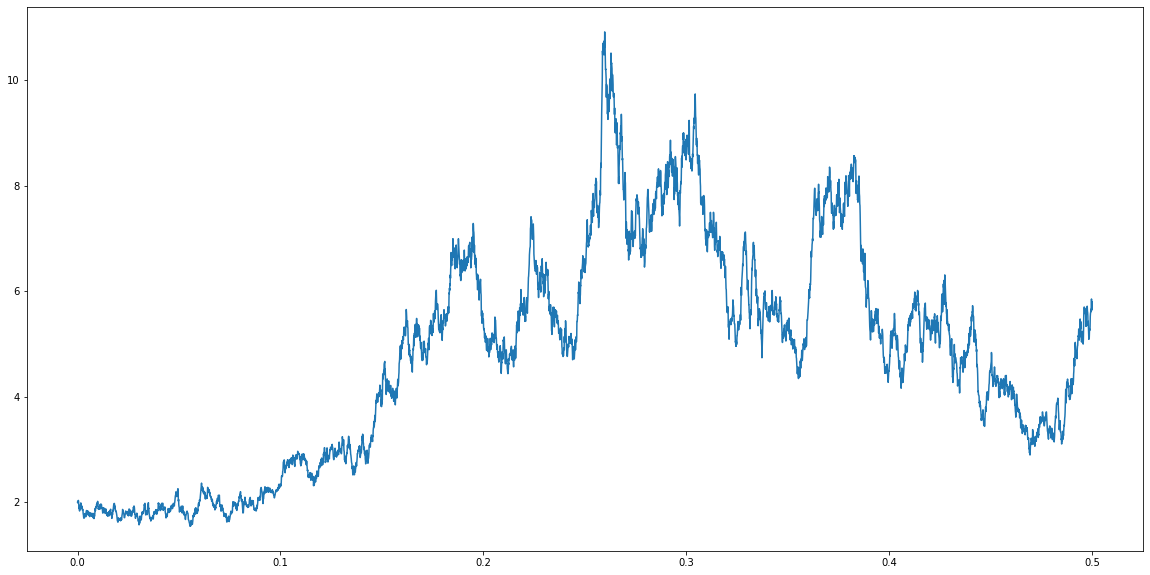
\includegraphics[width=2.95in]{images/path_1}}
	\subfigure[样本轨迹2]{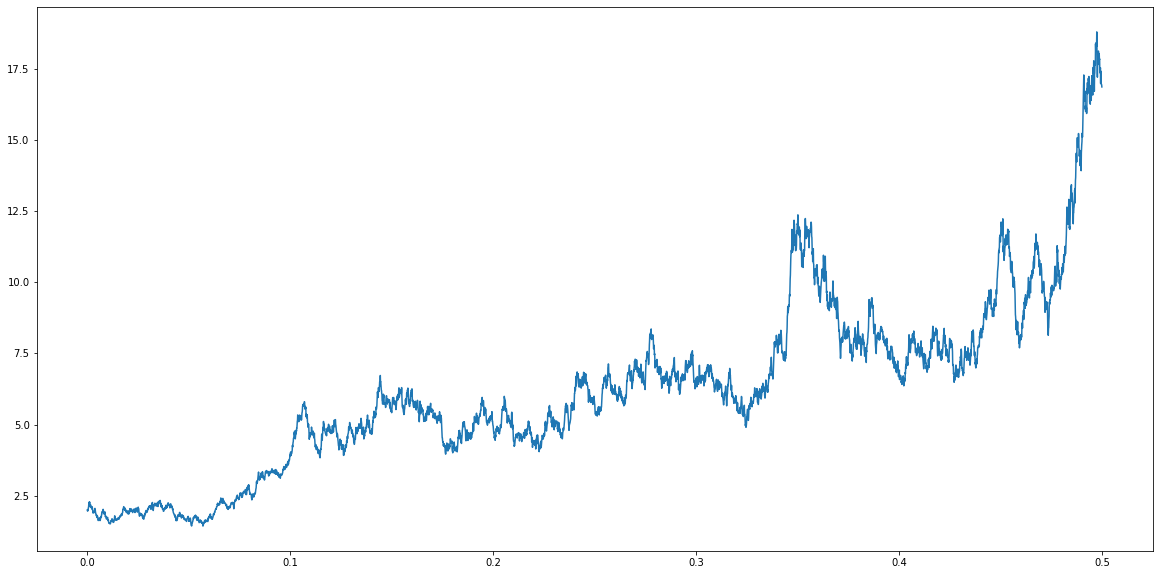
\includegraphics[width=2.95in]{images/path_2}}
	\caption{欧拉方法模拟几何布朗运动} 
	\vspace{.2cm}
	\label{path_1_2}
\end{figure}

一些数值测试表明,欧拉方法在该样例中是可靠的,见表\ref{tab_1},蒙特卡洛模拟的样本轨道数量为 $10^4$. 


\begin{table}[!htbp]
\centering
\begin{tabular}{r|c|c|c|c|c|c|c|c}
	方程参数 & 时间($T$) & $EX$ & $DX$& 步长($h$) & $E\overline X$ & $D\overline X$&$ E|X-\overline X| $   & $E(X-\overline X)^2$  \\
	\hline
	$X_0=2$&&&&             1e-2&2.402&43.00&7.27e-3&12.27 \\
	$b=2$&0.1&2.442&66.72&  1e-3&2.421&53.83&1.88e-3&1.361 \\
	$\sigma=5$&&&&          1e-4&2.425&58.45&5.18e-4&0.137 \\
	\hline
	$X_0=2$&&&&             1e-2&22.68&1911&1.187&117.7 \\
	$b=2$&0.5&24.36&3792&   1e-3&25.30&4634&0.214&31.06 \\
	$\sigma=5$&&&&          1e-4&23.98&4075&0.007&1.605 \\
	\hline
	$X_0=2$&&&&             1e-2&8.14e-5&5.26e-5&1.22e-4&1.37e-3 \\
	$b=2$&3&806.8&inf&      1e-3&5.09e-4&8.45e-4&5.93e-4&1.06e-3 \\
	$\sigma=5$&&&&          1e-4&2.47e-3&3.81e-2&1.57e-3&2.17e-2 \\
	\hline
	$X_0=2$&&&&             1e-2&0.7305&4.587&4.36e-3&0.1312\\
	$b=-2$&0.5&0.7357&3.458&1e-3&0.7454&3.605&2.93e-3&0.0181\\
	$\sigma=2$&&&&          1e-4&0.7165&3.145&6.92e-4&0.0013\\
	\hline
	$X_0=2$&&&&             1e-2&0.2694&1.907&9.73e-3&0.2106\\
	$b=-2$&1&2.707&3.926&   1e-3&0.2820&2.385&1.54e-3&0.0322\\
	$\sigma=2$&&&&          1e-4&0.2547&1.388&2.61e-4&0.0012\\
	\hline
	$X_0=2$&&&&             1e-2&2.26e-5&7.61e-7&1.18e-5&1.34e-6\\
	$b=-2$&5&9.080e-5&4.000&1e-3&1.38e-5&5.49e-8&7.75e-7&1.15e-9\\
	$\sigma=2$&&&&          1e-4&2.14e-5&3.01e-7&7.02e-8&7.0e-10\\
\end{tabular}
\vspace{.2cm}
\caption{欧拉方法的蒙特卡洛模拟} 
\label{tab_1}
\end{table}
注意到表\ref{tab_1}中,$D\overline{X}$ 不一定能收敛到 $DX$,但每条样本轨道上的误差的一阶矩和二阶矩是可以被 $h$ 控制的,且误差阶与上文计算的一致. 同时对 $b-\frac12 \sigma^2>0$ 的情况,时间 $T$ 取的稍大,会解曲线会爆炸增长;相应的,对 $b-\frac12 \sigma^2<0$ 的情况,会收敛到0. 

基于前文叙述的显式 Euler 格式,可以很自然的叙述出相应的隐格式 Euler 算法,此处简略,后文将介绍精度更高的方法,而此处隐格式算法的稳定性的讨论则过于冗长.



\subsection{Taylor  方法}
引入算子记号
\[
\begin{aligned} 
& \Lambda_k = \sigma_k ^ T \frac{\partial }{\partial x}  =  (\sigma_k,\frac{\partial}{\partial x}) = \sum_{i=1}^d \sigma_k^i \frac{\partial}{\partial x^i},\\
& L = \frac{\partial}{\partial t} + b^T \frac{\partial}{\partial x} + \frac12 \sum_{k=1}^m \sum_{i=1}^d \sum_{j=1}^d \sigma_k^i \sigma_k^j \frac{\partial^2}{\partial x^i \partial x^j}.
\end{aligned}
\]
称算子 $L$ 为 Lyapunov 算子. 

借助 \ito 公式和 Taylor 展开,对于光滑二元函数 $f(t,x)$,有
\begin{equation}\label{eq3.14}
f(T,X(T)) = f(t,x(t)) + \sum_{r=1}^m \int_t^T \Lambda_r f(\theta,X(\theta)) \md B_r(\theta) + \int_t^T Lf(\theta,X(\theta)) \md \theta.
\end{equation}
再对于 $\Lambda_rf$ 和 $Lf$ 做类似(\ref{eq3.14})的展开,得二阶展开表达式
\begin{equation}\label{eq3.15}
\begin{aligned}
	f(T,X(T)) = f  &+ \sum_{r=1}^m \Lambda_rf \int_t^T \md B_t(\theta) + Lf\int_t^T\md \theta\\
	&+\sum_{r=1}^m \int_s^T \left( \sum_{i=1}^m \int_t^\theta \Lambda_i\Lambda_r f(\theta_1,X(\theta_1))\md B_i(\theta_1) \right) \md B_r(\theta)\\
	&+\sum_{r=1}^m \int_t^T \left(  \int_t^\theta L\Lambda_r f(\theta_1,X(\theta_1))\md \theta_1\right) \md B_r(\theta) \\
	&+ \sum_{r=1}^m \int_t^T \left(  \int_t^\theta \Lambda_r Lf(\theta_1,X(\theta_1))\md B_r(\theta_1)\right) \md \theta \\
	&+\int_t^T \left( \int_t^\theta L^2 f(\theta_1,X(\theta_1)) \md\theta_1\right)\md \theta
\end{aligned} 
\end{equation}
此处 $f,\Lambda_rf,Lf$ 均指在 $(t,X(t))$ 处的值. 可以继续对于 $L^2f,L\Lambda_r,\Lambda_rL,\Lambda_i\Lambda_r$ 做类似(\ref{eq3.14})的展开,本节不继续赘述. 基于(\ref{eq3.15}), 有
\begin{equation}\label{eq3.16}
\begin{aligned} 
	f(t+h,X(t+h)) = f &+ \sum_{r=1}^m \Lambda_rf\int_t^{t+h} \md B_r(\theta) + Lf \int_t^{t+h} \md \theta \\
	& + \sum_{r=1}^m\sum_{i=1}^m \Lambda_i\Lambda_rf \int_t^{t+h} \md B_r(\theta) \int_t^\theta \md B_i(\theta_1)\\
	& + \sum_{r=1}^m\sum_{i=1}^m\sum_{s=1}^m \Lambda_s\Lambda_i\Lambda_r f
	\int_t^{t+h}\md B_r(\theta) \int_t^\theta \md B_i(\theta_1) \int_t^{\theta_1} \md B_s(\theta_2)\\
	&+\sum_{r=1}^m \Lambda_rLf \int_t^{t+h} \md \theta \int_t^\theta \md B_r(\theta_1)
	 +\sum_{r=1}^m L\Lambda_rf \int_t^{t+h} \md B_r(\theta) \int_t^\theta \md \theta_1\\
	&+L^2f\int_t^{t+h} \md \theta \int_t^\theta\md \theta_1 + R 
\end{aligned}
\end{equation}
$R$ 表示高阶项.取 $f(t,x)=x$,则有
\[
\Lambda_rf = \sigma_r,\qquad Lf=b.
\]
并计算积分式,带入(\ref{eq3.16})得 Taylor 方法:
\begin{equation}\label{eq_taylor}
\begin{aligned}
\overline{X}_{t,x} (t+h) = x &+ bh+\sum_{r=1}^m \sigma_r(B_r(t+h)-B_r(t))\\
	&+\sum_{r,i=1}^m \Lambda_i\sigma_r \left( \frac12 (B_r(t+h) - B_r(t))^2 - \frac 12 h \right)\\
	&+\sum_{r=1}^m \Lambda_rb \int_t^{t+h} B_r(\theta)-B_r(t) \md \theta\\
	&+\sum_{r=1}^m L\sigma_r  \int_t^{t+h} (\theta - t)\md B_r(\theta)\\
	&+\sum_{r,i,s=1}^m \Lambda_s\Lambda_i\sigma_r \int_t^{t+h} \left(
	  \int_t^\theta B_s(\theta_1) - B_s(t) \md B_i(\theta_1)\right)\md B_r(\theta)\\
	&+\frac{Lbh^2}{2}
\end{aligned}
\end{equation}
对 $X_{t,x}(t+h)$ 的这种展开,也称为 Wagner-Platen 展开. 注意到存在无法精确计算的积分式,因此实际操作的时候,会引入数值积分并引入进一步的误差. 

\paragraph*{ 例子} 考虑线性随机微分方程系统
\begin{equation}\label{eq3.18}
	\md X = A(t) X \md t + \sum_{r=1}^m B_r(t) X\md B_r(t),\qquad  t\in [0,T].
\end{equation}
这里 $A(t),B_r(t)$ 均为 $d\times d$ 的矩阵函数. 由
\[
\Lambda_i\sigma_r(t,x) = B_i(t) x\times \frac{\partial}{\partial x} (B_r(t)x) = B_r(t)B_i(t)x.
\]
其余项在算子作用下变成0,因此数值格式为:
\[
\begin{aligned} 
	\overline{X}_{t,x}(t+h) =x&+\sum_{r=1}^m B_r(t) x \Delta_tB_r(h) + A(t)x h 
	+ \frac12\sum_{r=1}^m B_r^2(t) x (\Delta_t^2 B_r(h)-h)\\
	&+\sum_{r=2}^m\sum_{i=1}^{r-1} B_i(t)B_r(t) x \Delta_t B_i(h) \Delta_t B_r(h).
\end{aligned}
\]
在这个例子中,包含 $m$ 个布朗运动,需要特别注意 $B_i,B_j$ 在 $i\neq j$ 时相互独立,而在 $i=j$ 时,协方差非零. 


对于自治随机微分方程,函数 $b,\sigma$ 是仅关于 $x$ 的函数. 此处介绍一种 Taylor 格式,其具有$\frac32$阶的整体误差精度.
\begin{equation}\label{Taylor}
\begin{aligned}
\overline{X}_{t,x} (t+h)=& x+h b + \sigma \Delta_B +\frac12 \sigma'\sigma (\Delta_B^2-h) + \frac12 \left( b'b + \frac 12 b''\sigma^2 \right) h^2\\
&+\frac{1}{2}(b'\sigma)
\left(\Delta _B +\frac{1}{\sqrt{3}} \int _t^{t+h} B_\theta \md \theta\right) h\\
&+\frac{1}{2}\left( \sigma'b+\frac12 \sigma ''\sigma^2 \right)
\left(\Delta _B - \frac{1}{\sqrt{3}} \int _t^{t+h} B_\theta \md \theta\right) h\\
&+\frac16 (\sigma'^2 \sigma + \sigma''\sigma^2) (\Delta_B^3-3h\Delta _B)
\end{aligned}
\end{equation}
对于一些构造良好的例子,数值格式(\ref{Taylor})中不可精确积分的表达式正好可以消去,从而得到可以显式数值格式. 




\subsection{Milstein 格式 、中点公式、隐格式}
Milstein 格式是特殊的Taylor方法,对于自治随机微分方程(\ref{SODE}),有 $\Lambda_ig_r = \Lambda_rg_i$,称数值格式为
\[
\begin{aligned} 
	\overline{X}_{t,X}(t+h) = x+&f(x)h + \sum_{r=1}^m g_r(x) \Delta_t B_r(h) - \frac12\sum_{r=1}^m \Lambda_rg_r(x)[ (\Delta_t B_r(h))^2-h] \\
	+&\sum_{i=1}^m \sum_{r=i+1}^m\Lambda_ig_r(x) \Delta_t B_i(h) \Delta_t B_r(h).
\end{aligned} 
\]
Milstein 格式,其中 $\Lambda_ig_r(x) = (g_r(x))^Tg_i(x)$. Milstein 格式具有1阶整体误差精度. 

%\subsection{中点公式}
自治随机微分方程(\ref{SODE})的中点格式为
\begin{equation}\label{mid_point}
\overline{X}_{t,x}(t+h) = x + b\left( \frac{x+\overline{X}}{2}\right) h  - \frac12 \sum^q_{r=1} \frac{\partial \sigma_r}{\partial x} \sigma_r \left( \frac{x+\overline{X}}{2}\right) h  + \sum^q_{r=1} \sigma_r \left(\frac{x+\overline X}{2} \right)  \Delta_t B_r(h),
\end{equation}
在线性增长条件和 Lipschitz 条件成立的情况下,中点公式具有1阶整体误差精度,见文献\cite{kutta_1,kutta_2}. 中点公式是隐格式,一般具有更好的数值稳定性. 但相对应的,其向前的差分往往不能直接导出,数值实现会复杂一些. 

文献\cite{Implicit_Taylor,Implicit_Taylor_1,Implicit_Taylor_2}给出了自治随机微分方程(\ref{SODE})的半隐 Milstein 格式和半隐 Taylor格式,见(\ref{eq3.20}). 可以看出这两种隐格式与对应的显格式几乎是一致的,仅是取点有所不同. 同样的数值精度下,具体选择哪种格式则依据实际需求. 本文第5节介绍的保守恒量的数值格式全部为隐格式, 
\begin{equation}\label{eq3.20}
\begin{aligned}
x_{n+1} = x_n+&b(x_{n+1})h + \sigma(x_n) \Delta B + \frac12 [\sigma^\prime \sigma] (x_n) ((\Delta B)^2-h) \\
x_{n+1} = x_n+&b(x_{n+1})h + \sigma(x_n) \Delta B + \frac12 [\sigma^\prime \sigma] (x_n) ((\Delta B)^2-h)\\
			 +&\frac{1}{2} [b^{\prime} \sigma](x_n)\left(\frac{\Delta B'}{\sqrt{3}}-\Delta B\right)h
			 -\frac{1}{2}\left[b^{\prime} b+\frac{1}{2} f^{\prime \prime} \sigma^{2}\right](x_{n+1}) h^2\\
			 +&\frac12\left[\sigma^{\prime} +\frac12 \sigma^{\prime \prime} \sigma^{2}\right](x_n)\left(\Delta B-\frac{\Delta B'}{\sqrt{3}}\right) h\\
			 +&\frac{1}{6}\left[\sigma^{\prime 2} \sigma+\sigma^{\prime \prime} \sigma^{2}\right](x_n) (\left(\Delta B\right)^3-3 h \Delta B )
\end{aligned}
\end{equation}
这里的 $\displaystyle \Delta_B' = \frac{1}{\sqrt{3}} \int _t^{t+h} B_\theta \md \theta$,由于随机分析中的等距公式,其服从均值为0、方差为 $\frac13$ 的正态分布. 
自治随机微分方程的半隐 Milstein 格式和半隐 Taylor格式分别具有1阶和 $\frac32$阶的整体误差. 


\section{多步法}

%\subsection{Runge-Kutta 方法}
此处仅介绍一维自治随机微分方程(\ref{SODE})的随机 Runge-Kutta 方法,更一般问题的多步法见文献\cite{book_kutta}.

s步Runge-Kutta方法定义如下:
\begin{equation}\label{kutta}
\begin{aligned}
X_{n+1} = X_n + & \sum_{i=1}^s \alpha_i b(H_i^{(0)}) h + \sum_{i=1}^s\gamma_i^{(1)} \sigma(H_i^{(1)})\Delta_tB \\
+ & \sum_{i=1}^s \gamma_i^{(2)} \sigma(H_i^{(1)})\frac1{\sqrt h} \int_t^{t+h}\md B(\theta_1) \int_t^{\theta_1} \md B(\theta)
\end{aligned}
\end{equation}
其中
\[
\begin{aligned}
H_{i}^{(0)} &=X_{n}+\sum_{j=1}^{i-1} A_{i j}^{(0)} b\left(H_{j}^{(0)}\right) h+\sum_{j=1}^{i-1} B_{i j}^{(1)^{(0)}} \sigma\left(H_{j}^{(1)}\right) \Delta_tB \\
H_{i}^{(1)} &=X_{n}+\sum_{j=1}^{i-1} A_{i j}^{(1)} b\left(H_{j}^{(0)}\right) h+\sum_{j=1}^{i-1} B_{i j}^{(3)^{(1)}} \sigma\left(H_{j}^{(1)}\right) \sqrt{h}
\end{aligned}
\]
使用 Butcher-Arrays 形式表示 
\begin{table}[!htbp]
\centering
\begin{tabular}{p{1cm}<{\centering} | p{2cm}<{\centering} | p{2cm}<{\centering} |p{2cm}<{\centering}}
	\multirow{2}{*}{} & $A^{(0)}$ & $B^{(1)^{(0)}}$ & \\
	\cline{2-4}
	\rule{0pt}{13pt} & $A^{(1)}$ & $B^{(3)^{(1)}}$ & \\
	\hline
	\rule{0pt}{15pt} $(p_{_D} , p_{_S})$& $\alpha^T$ & $\gamma^{(1)^T}$ & $\gamma^{(2)^T}$\\
\end{tabular}
\end{table}
这些参数需要满足28个方程\cite{book_kutta}. 
即使对于确定性的微分方程,Runge-Kutta 格式系数的计算也相当繁琐,而对于随机微分方程,则计算复杂度更是大大提升. 
这里直接介绍两种解:
\begin{table}[!htbp]
	\centering
	\begin{tabular}{p{1cm}<{\centering} | p{2.5cm}<{\centering} | p{2.5cm}<{\centering} |p{2cm}<{\centering}}
		\multirow{2}{*}{}
		\rule{0pt}{30pt} &  
		$\begin{matrix}	&&A^{(0)}\\\frac23 &&\\-\frac13&1& \end{matrix}$& 
		$\begin{matrix} &&B^{(1)^{(0)}} \\ 1&&\\0&0&  \end{matrix}$ & \\
		\cline{2-4}
		\rule{0pt}{30pt} & 
		$\begin{matrix} &&A^{(1)} \\ 1&&\\1&0& \end{matrix}$ & 
		$\begin{matrix} &&B^{(3)^{(1)}} \\ 1&&\\-1&0&\end{matrix} $ & \\
		\hline
		\rule{0pt}{15pt} $(3,2)$ &  
		$\begin{matrix} \frac14&\frac12&\frac14 &  \end{matrix}$ & 
		$\begin{matrix} \frac12&\frac14&\frac14 ~& \end{matrix}$ & 
		$\begin{matrix} 0&\frac12&-\frac12   \end{matrix}$\\
	\end{tabular}
\vspace{.2cm}
\caption{SRK 格式一} \label{SRK1}
\end{table}
\begin{table}[!htbp]
	\centering
	\begin{tabular}{p{1cm}<{\centering} | p{2.5cm}<{\centering} | p{2.5cm}<{\centering} |p{2cm}<{\centering}}
		\multirow{2}{*}{}
		\rule{0pt}{30pt} &  
		$\begin{matrix}	&&A^{(0)}\\\frac23 &&\\-\frac12&\frac12& \end{matrix}$& 
		$\begin{matrix} &&B^{(1)^{(0)}} \\ 0&&\\1&0&  \end{matrix}$ & \\
		\cline{2-4}
		\rule{0pt}{30pt} & 
		$\begin{matrix} &&A^{(1)} \\ \frac14&&\\0&\frac14& \end{matrix}$ & 
		$\begin{matrix} &&B^{(3)^{(1)}} \\ -\frac12&&\\\frac12&0&\end{matrix} $ & \\
		\hline
		\rule{0pt}{15pt} $(3,2)$ &  
		$\begin{matrix} -\frac14&\frac34&\frac12 &  \end{matrix}$ & 
		$\begin{matrix} -1&1&1& \end{matrix}$ & 
		$\begin{matrix} 0&-1&1  \end{matrix}$\\
	\end{tabular}
\vspace{.2cm}
\caption{SRK 格式二} \label{SRK2}
\end{table}


表\ref{SRK1}和表\ref{SRK2}中的 $(p_{_D} , p_{_S})=(3,2)$ 表示该数值格式对确定性的微分方程具有3阶误差精度,而对随机微分方程则具有2阶误差精度. 

尽管精度相同,但不同的格式会具有不用的数值性质. 在文献\cite{kutta_6,kutta_7,kutta_8,kutta_9}中,给出了针对随机Hamilton系统的随机Runge-Kutta方法. 

\section{谱方法}
在确定性偏微分方程中,有限元方程、谱方法都是常用的数值方法. 在随机系统中,也期望传统的数值方法能用于求解该类随机微分方程. 谱方法用于处理算子方程,因此需要将微分方程形式的 SDE 用算子形式重述. 本节介绍随机Galerkin方法和Wong-Zakai逼近方法. 目前的谱方法不太适合用于求解自治随机
常微分方程(\ref{SODE}),更适用于分析和求解SPDE,本节简单介绍谱算法的思路. 





\subsection{随机 Galerkin 方法}
给定随机控制问题 $\md X(t,\omega)  = b(t,X,\omega) \md t$,将其处理为下面的SDE方程
\[
	\left\{
	\begin{aligned}
	&\frac{\partial X}{\partial t}(t,\omega) = b (t,X,\omega), &(0,T]\times \R    \\
	&\mB (X)=0, &\partial(0,T]\times \R     \\
	&X=X_0, & \{t=0\} \times \R
	\end{aligned}
	\right.
\]
这里 $\omega$ 为正态随机变量. 
与之前不同的是,该问题的随机项落在漂移函数 $b$ 内部,而不含扩散项 $\md B_t$. 这使得该类问题的样本轨道重新成为有界变差函数. 
选取基函数空间 $\{ H_{k}(\omega) \}$,$H_k$ 是以 $\omega$ 为变量的 Herimite 多项式. 此时有
\[
	E[H_i(\omega) H_j(\omega)] = \delta_{ij} \gamma_i,
\]
若 $\omega$ 服从其它的随机分布,则基函数空间的选择也会随之变动,见文献\cite{book_buqueding}. 
问题的解在基函数空间中的投影为:
\[
	X_{_N}(t,\omega) = \sum_{i=0}^N \hat b_i(t) H_i (\omega),\qquad
	\hat b_i(t) = \frac1{\gamma_i} E[X(t,\omega)H_i(\omega)]
\]
问题满足下面的方程组:
\[
\left\{
\begin{aligned}
&E\left[\frac{\partial X_{_N}(t,\omega)}{\partial t} H_k(\omega)\right] = E[b(t,X,\omega) H_k(\omega)],\\
&E[\mB(X_{_N}) H_k(\omega)] = 0,\\
&\hat b_k(0) = \hat b_{0,k}\\
\end{aligned}
\right.
\qquad \forall k \in \{0,1,\cdots,N\}.
\]
求解该方程组,根据 $\{\hat b_i(t)\}_{i=0}^N$ 即可得原问题的解. 对于多维随机变量的情况,通过修改基函数空间也可以实现. 
 
 
\subsection{Wong-Zakai逼近}
Wong-Zakai逼近用于计算随机演化方程的数值解,与随机 Galerkin 方法一样,都只适用于不含 $\md B_t$ 项的随机控制方程. 对于方程
\begin{equation}\label{SEE}
	L u(t,x) = b(u(t,x)) + \xi (t,x) ,\qquad (t,x) \in [0,T]\times (0,1),
\end{equation}
给定 Dirichlet 边界条件 $u(t,0) = u(t,1) = 0$ 或 Neumann 边界条件 $\partial_x u(t,0) = \partial_x u(t,1) = 0$. 将时空区域离散成 $m\times n$ 份,得 $\xi(t,x)$ 的Wong-Zakia近似式:
\begin{equation}\label{WongZakai}
	\tilde \xi (t,x)  =  \sum_{i=0}^{m-1} \sum_{j=0}^{n-1}\left[ \frac 1{mn}\int _ {\frac {iT}m}^{\frac{(i+1)T}m} \int_{\frac{j}{n}}^{\frac{j+1}n} \xi(ds,dy)\right] \chi_{i,j}(t,x)
\end{equation}
将(\ref{WongZakai})带入(\ref{SEE}),得近似的正则化方程
\begin{equation}\label{new_SEE}
	L \tilde{u}(t,x) = b(\tilde{u}(t,x)) + \tilde \xi (t,x). 
\end{equation}
注意到 $\xi$ 是分割网格上的分段常值函数. 下面给出两个实例.

\subsubsection*{随机热方程的半离散 Galerkin 有限元方法}

考虑算子 $L=\partial_t - \partial_{xx}$,称方程(\ref{SEE})为随机热方程(SHE),离散的空间上自然构造出有限元空间 $V_h$. 定义投影算子 $P_h:L^2\mapsto V_h$,使得
\[
(P_h u,v) = (u,v),\qquad \forall u\in \mathbb L^2,v\in V_h.
\]
半离散 Galerkin 有限元逼近的目标是找到函数 $\tilde{u}_{_h} \in V_h$,使得 $\tilde u_{_h}(0) = P_h \tilde u_0$,且
\[
\md \tilde u_{_h}(t) = \Delta_h \tilde u_{_h}(t) \md t + 
P_h \left( b(\tilde u_{_h}(t))  + \tilde \xi (t)\right) \md t.
\]


\subsubsection*{随机波动方程的谱Galerkin方法}

考虑算子 $L=\partial_{tt} - \partial_{xx}$,称方程(\ref{SEE})为随机波动方程(SWE). 取合适的基空间 $V_{_N} = \operatorname{span}\{\varphi_i\}_{i=1}^N$,正交投影算子 $P_N:L^2\mapsto V_{_N}$ 满足:
\[
(P_{_N} u,v) = (u,v) ,\qquad \forall v \in V_{_N}. 
\]
谱 Galerkin 方法的目标就是找到 $\tilde{u}_{_N}$,使得 $\tilde{u}_{_N}(0) = P_{_N} u_0$,且对任意 $t>0,v\in V_{_N}$,有
\[
\left(\partial_{t} \tilde{u}_{_N}(t), v\right)=\left(P_{_N} v_{0}, v\right)+\int_{0}^{t}\left(\tilde{u}_{_N}(s), \Delta v\right) d s+\int_{0}^{t}\left(b\left(\tilde{u}_{_N}(s)\right)+\tilde{\xi}(s), v\right) d s
\]
这两个例子都仅对空间离散操作,而不离散时间. 和之前的随机 Galerkin 方法一样,不能处理带 $\md B_t$ 项的随机微分方程. 















 
  % SDE的解与数值解法
  % !TeX encoding = UTF-8
\chapter{解的长时间演化行为}\label{chap4}

\section{概率解与稳定解}

类似于离散或连续Markov模型,随机过程长时间演化有可能收敛到一个均匀的概率分布,即极限状态与平稳状态存在且两者一致. 目前对如下形式的 SDE 已经有了一定的理论成果,
\begin{equation}\label{eq_sde_fokker}
	\md X_t = b(X_t) \md t + \sigma(X_t) \md B_t,\qquad  x\in \R^d. 
\end{equation}
注意到它是自治随机偏微分方程,也就是说,其解的转移过程可以用一个Markov转移半群来表述\cite{semi_group_1,semi_group_2},而与时间项 $t$ 无关. 
借助 Feynman-Kac 表示,它可以与 Fokker-Planck 型确定型微分方程建立起紧密的联系. 令 $(a^{ij}) := \frac12 \sigma\sigma^T$. Fokker-Planck 方程的形式为:
\begin{equation}\label{eq_fokker}
	\partial_t u = Lu := \sum_{i,j=1}^d \partial^2_{ij} (a^{ij}u) - \sum_{i=1}^d \partial_i (b^ix),\qquad
	t>0,x \in \R^d.
\end{equation}

我们利用(\ref{eq_fokker})来定义(\ref{eq_sde_fokker})的测度意义下的弱解和稳定解.首先定义 Fokker-Planck 算子的伴随算子
\begin{equation}\label{eq4.3}
	\mL = \sum_{i,j}a^{ij} \partial_{ij}^2  + \sum_i b^i \partial_i
\end{equation}

\begin{definition}[测度解]
	令 $\nu$ 是 $\R^n$ 上的Borel测度. 我们称一族Borel测度 $\mu = (\mu_t)_{t\in [0,T]}$ 是问题(\ref{eq_sde_fokker})的初值为 $\nu$ 的测度解,若 $\mu_0=v$,$a^{ij},b^i \in L^1_{\mathrm{loc}}(\R^n,\md \mu_t \md t) \quad \forall i,j $ 且下面恒等式在$[0,T]$上几乎处处成立
	\[
	\int_{\R^n} \phi \md \mu_{t}=\int_{\R^n} \phi \md \nu + \lim _{\varepsilon \to 0^{+}} \int_{\varepsilon}^t \int_{\R^n} \mL \phi \md \mu_s \md s,\quad \phi \in C_{0}^{\infty}(\R^n) .
	\]	
	进一步地,若 $\mu_t(\R^n) = 1$,则称为概率解. 
\end{definition}

此处的概率解 $\mu=(\mu_t)$ 代表问题(\ref{eq_sde_fokker})在初值 $X_0$ 服从概率分布 $\mu_0$ 时解 $(X_t)$ 的概率分布. 因而测度具有归一化的性质. Feynman-Kac 表示的成立对漂移项和扩散项函数有一定的要求,此处不再多做介绍. 
Fokker-Planck 方程的概率解的存在性和唯一性已经在很多文献中进行了讨论\cite{zongshu2-24,zongshu2-26},包括系数函数与时间 $t$ 相关的问题. 
接下来定义样本轨道的集合的稳定状态. 这里在概率意义下给出稳定解的定义:






\begin{definition}[稳定解]
	$\R^n$ 上的 Borel 测度 $\mu$ 称为稳定解,若 Fokker-Planck 方程(\ref{eq_fokker})对应的算子 $L$ 满足 $L\mu = 0$,即
	$b_i \in L^1_{\text{loc}}(\R^n , \mu), \forall i$ 且
	\[
	\int_{\R^n} \mL \phi \md \mu = 0,\qquad  \forall \phi \in C_0^\infty(\R^n).
	\]
\end{definition}

不同于之前从样本轨道的角度理解方程的解,概率解和稳定解从所有样本轨道的角度出发理解随机微分方程解的性质. 







\begin{definition}[Lyapunov 型函数]
	对 $\R^d$ 上的非负连续函数 $U \in C^2(\R^d)$,记水平集
	\[
	\Omega_\rho = \{ x\in \R^d :U(x) < \rho \},\qquad \rho > 0,
	\]
	其为准紧集. 
	\begin{enumerate}
		\item 称无界函数 $U$ 为 Lyapunov 型函数,若存在常数 $C_1,C_2,\rho_m > 0$ 使得
		\[
		\mathcal{L} U(x) \leq C_{1}+C_{2} U(x), \quad x \in \R \backslash \overline {\Omega}_{\rho_{m}}
		\]
		\item 称无界函数 $U$ 为 Lyapunov 函数,若存在常数 $\gamma,\rho_m>0$ 使得
		\[
		\mathcal{L} U(x) \leq-\gamma, \quad x \in \R \backslash \overline {\Omega}_{\rho_{m}}
		\] 
		\item 称无界函数 $U$ 为强 Lyapunov 型函数,若存在常数 $C_1,C_2,\rho_m > 0$ 使得
		\[
		\mathcal{L} U(x) \leq C_{1}-C_{2} U(x), \quad x \in \R \backslash \overline {\Omega}_{\rho_{m}}
		\]
	\end{enumerate}
\end{definition}

这三种条件逐步加强,概率解的存在性和唯一性的定理如下:

\begin{theorem}
	若存在算子 $\mL$ 对应的 Lyapunov 型函数,则下列叙述成立:
	\begin{enumerate}
		\item
			方程(\ref{eq_fokker})存在初值概率分布为 $\nu$ 下的概率解 $(\mu_t)_{t\in[0,\infty)}$,且对任意 $\phi \in C_0^\infty(\R^d)$,映射 $t\mapsto \displaystyle \int_{\R} \phi \md \mu_t$ 是连续的;  
		\item 
			若 $(\tilde \mu_t)_{t\in [0,\infty)}$ 也是方程(\ref{eq_fokker})在初值概率分布为 $\nu$ 下的概率解,且满足映射 $t\mapsto \displaystyle \int_{\R} \phi \md \tilde\mu_t$ 是连续的对任意 $\phi \in C_0^\infty(\R^d)$ 成立,则 $\tilde \mu_t = \mu_t,\quad  \forall t>0$. 
	\end{enumerate}
\end{theorem}



上述定理说明了方程(\ref{eq_fokker})的概率解的存在唯一性,Feynman-Kac 公式表明随机的SDE的解与Fokker-Planck方程的解能关联起来. 因此SDE到达稳定状态时,$\partial_t\mu(t,x) = 0$. 注意到
\[
\int_{\R^n} \mL \phi \md \mu = \int_{\R^n} (\mL \phi, \mu(t,x)) \md x= 
\int _{\R^n} (\phi,L\mu(t,x)) \md x = 0.
\]
因此在弱意义下,有 $\partial_t \mu = L\mu = 0$. 















\section{稳定解验证}
%文献指出\cite{Fokker_Planck}指出,稳定解存在和收敛的充分条件是存在区域范围上无界非负 Lyapunov函数 $U(x)$ 和常数 $C_1,C_2>0 $,使得
%\[
%\mL U(x) \le C_1 - C_2 U(x) \qquad \text{或} \qquad 
%\mL U(x) < -C_1.
%\]


文献\cite{Fokker_Planck}指出,在 Lyapunov 条件下,自治随机微分方程(\ref{SODE})存在稳定解,且概率解在强 Lyapunov 条件下以指数速率收敛到稳定解. 
\begin{theorem}
	下面叙述成立:
	\begin{enumerate}
		\item
			若存在算子 $\mL$ 对应的无界 Lyapunov 函数,当 $t\to\infty$ 时,方程(\ref{eq_fokker})的任意测度解 $(\mu_t)_{t\in[0,\infty)}$ 均强收敛到唯一的稳定解 $\mu^*$,即对任意 Borel 可测集 $B \in \R^d$,有
			 \[
			 \mu_t(B) \to \mu^*(B),\qquad t\to \infty.
			 \]
		\item
			若存在算子 $\mL$ 对应的无界强 Lyapunov 函数,当 $t\to\infty$ 时,无论初值测度 $\nu$ 如何,测度解 $(\mu_t)_{t\in[0,\infty)}$  均指数收敛到唯一的稳定解 $\mu^*$,即存在常数 $C,r > 0$,使得
			\[
			\left\|\mu_{t}-\mu^{*}\right\|_{\operatorname{TV}} \leq C e^{-r t}, \quad t \geq 0,
			\]
			这里 $\|\cdot\|_{\operatorname{TV}} $ 表示全变差范数. 
	\end{enumerate}
\end{theorem}



简单看两个稳定解存在的例子和一个稳定解不存在的例子.

\subsection*{例1}
考虑方程
\[
\md x = bx \md t + \sqrt{2\sigma(x^2+1)} \md B_t,
\]
其中 $\sigma > b > 0$. 则其对应的 Fokker-Planck 方程为
\[
\partial_t = Lu := \partial_{xx} (\sigma(x^2+1)u) - \partial_x (bxu).
\]
取 $U(x) = \ln(x^2+1)$,伴随算子 $\mL = \sigma(x^2+1)\partial_{xx} + bx\partial_x$,有
\[
\mL U(x) = -\frac{2(\sigma-b) x^{2}-2 \sigma}{x^{2}+1} \le -(\sigma-b).
\]
满足 Lyapunov 条件,因此稳定解存在. 取参数$(b,\sigma)=(2,5)$,有偏初值 $X_0=10$,即 $P(X_0 = 10) = 1$,对 $50000$ 条样本轨道进行模拟,采用Milstein格式,结果见图\ref{path_4_1}和\ref{measure_4_1}.
一直模拟到 $T=100$,解始终维持 $T=5$ 时的形态. 再看另一个稳定解的例子. 

若不考虑噪声项,则 $x_t = x_0 e^{bx}$,随机系统退化为一个指数爆炸的系统,但引入充分大($\sigma>b$)的噪声项后,数值实验表明尽管样本轨道的二阶矩是发散的,但 $t$ 时刻绝大部分的点会落于 $[-10,10]$ 内. 

\begin{figure}[!htbp]
	\centering 
	\subfigure[T=0.001]{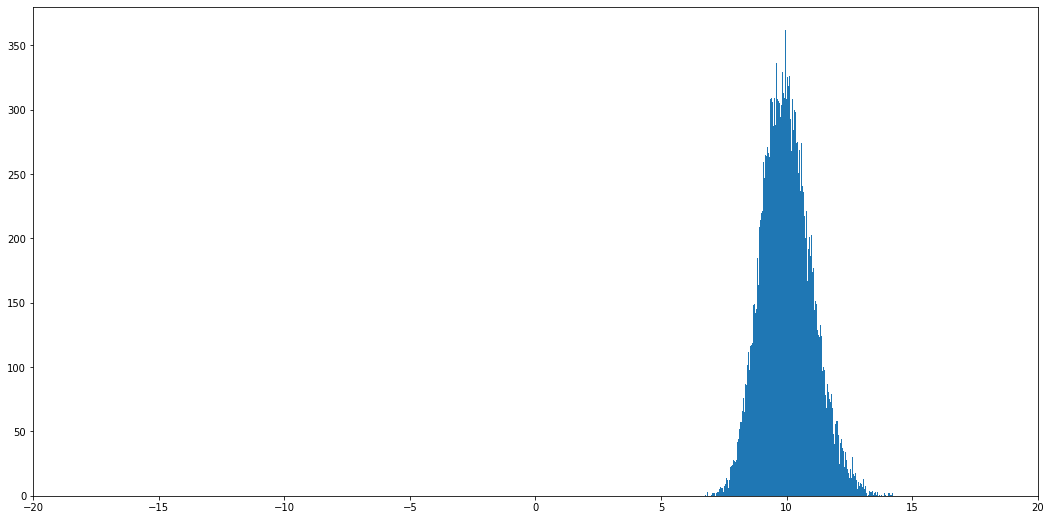
\includegraphics[width=2.95in]{images/4.1/fig_4.1(T=0.001)}}
	\subfigure[T=0.005]{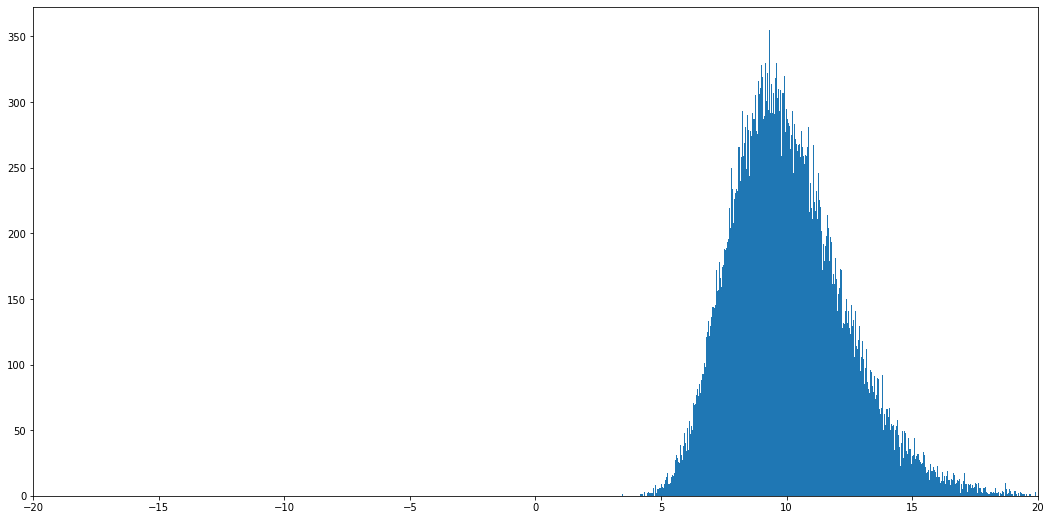
\includegraphics[width=2.95in]{images/4.1/fig_4.1(T=0.005)}}
	\subfigure[T=0.01]{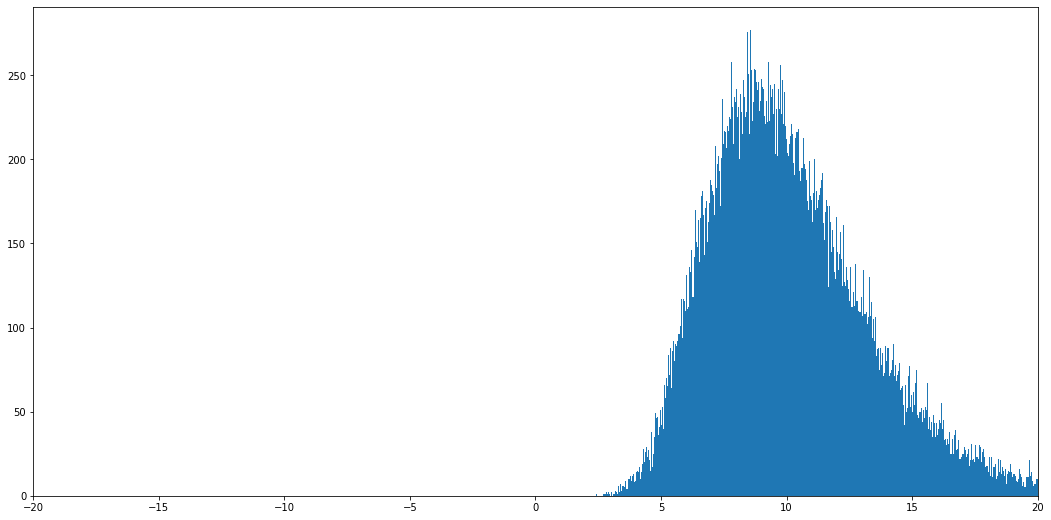
\includegraphics[width=2.95in]{images/4.1/fig_4.1(T=0.01)}}
	\subfigure[T=0.05]{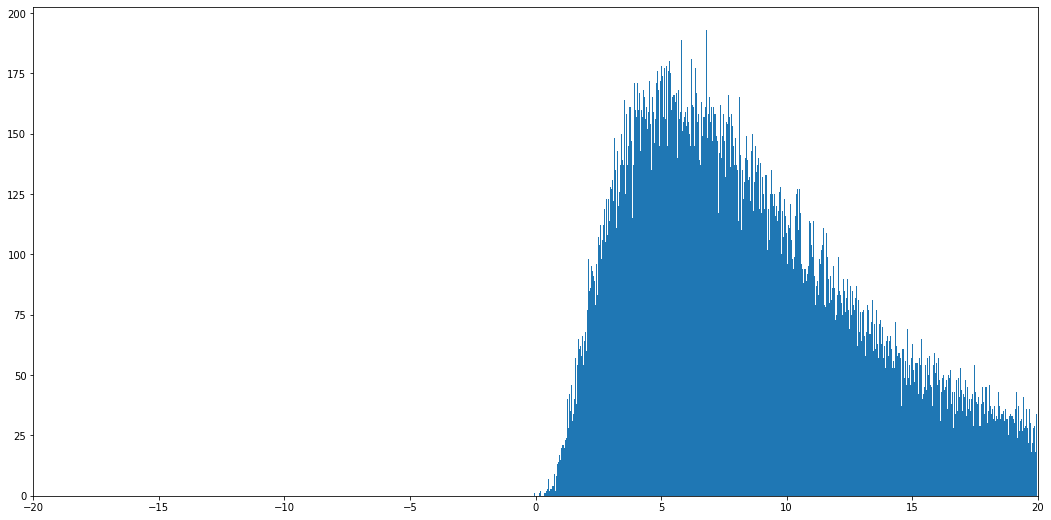
\includegraphics[width=2.95in]{images/4.1/fig_4.1(T=0.05)}}
	\subfigure[T=0.1]{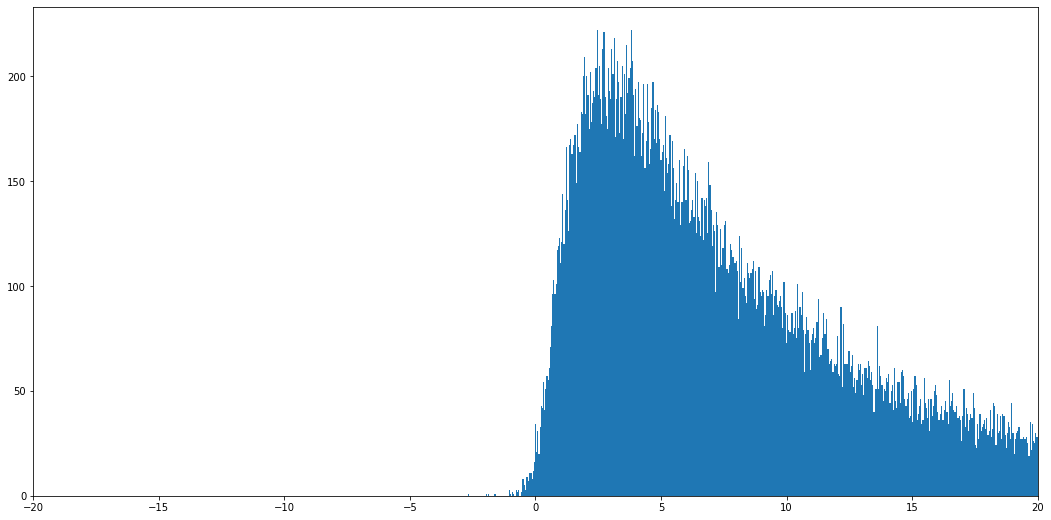
\includegraphics[width=2.95in]{images/4.1/fig_4.1(T=0.1)}}
	\subfigure[T=0.5]{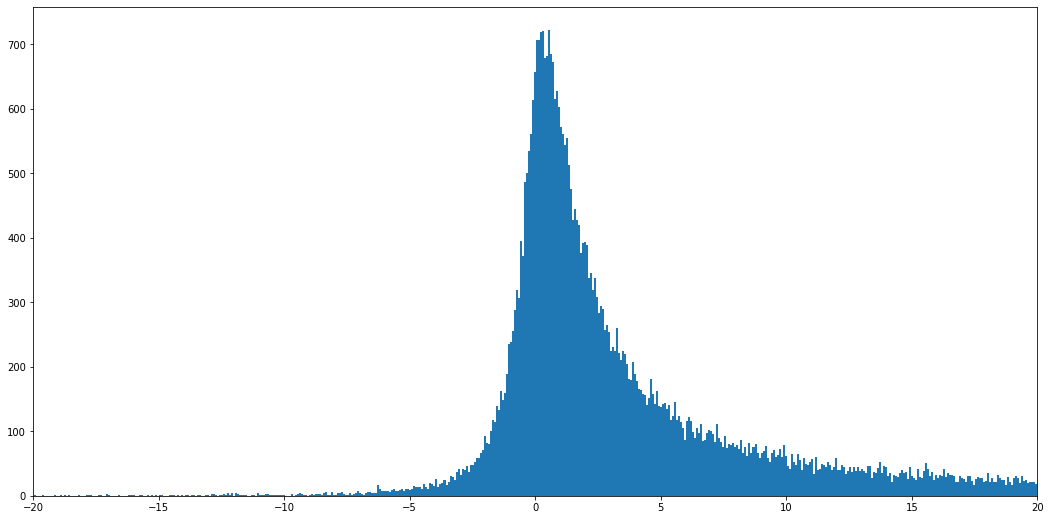
\includegraphics[width=2.95in]{images/4.1/fig_4.1(T=0.5)}}
	\subfigure[T=1]{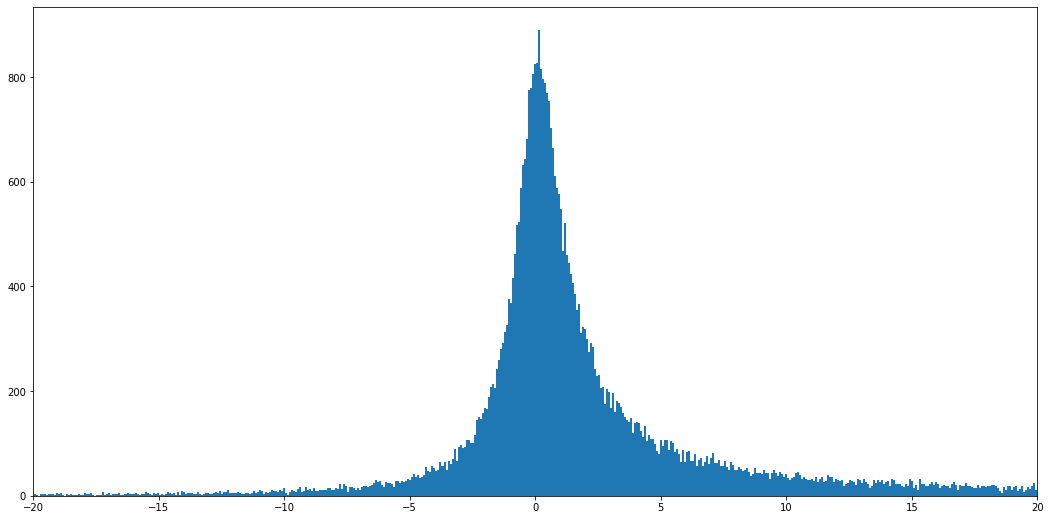
\includegraphics[width=2.95in]{images/4.1/fig_4.1(T=1)}}
	\subfigure[T=5]{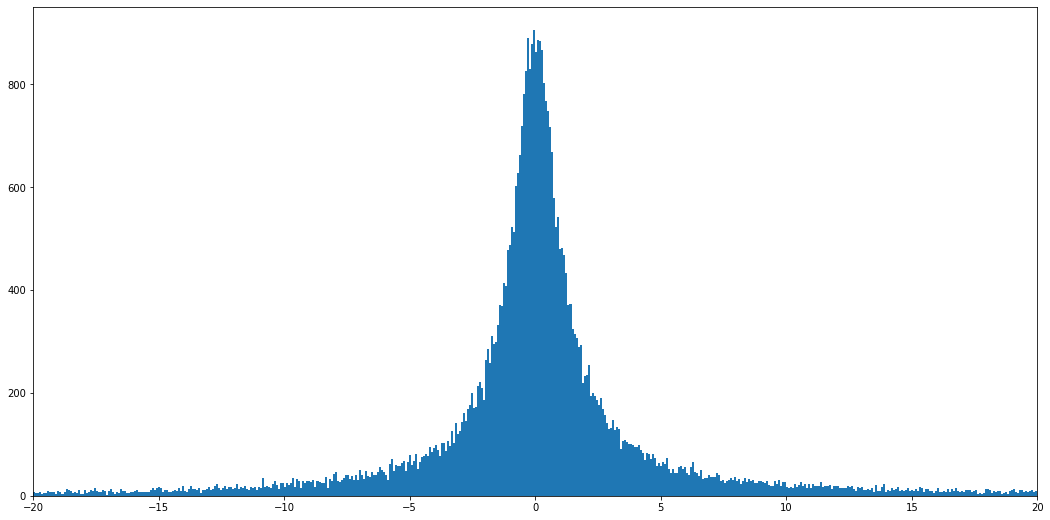
\includegraphics[width=2.95in]{images/4.1/fig_4.1(T=5)}}
	\centering
	\vspace{.2cm}
	\caption{稳定解的概率分布(一)}
	\label{measure_4_1}
\end{figure}

\begin{figure}[!htbp]
	\centering 
	\subfigure[样本轨迹1]{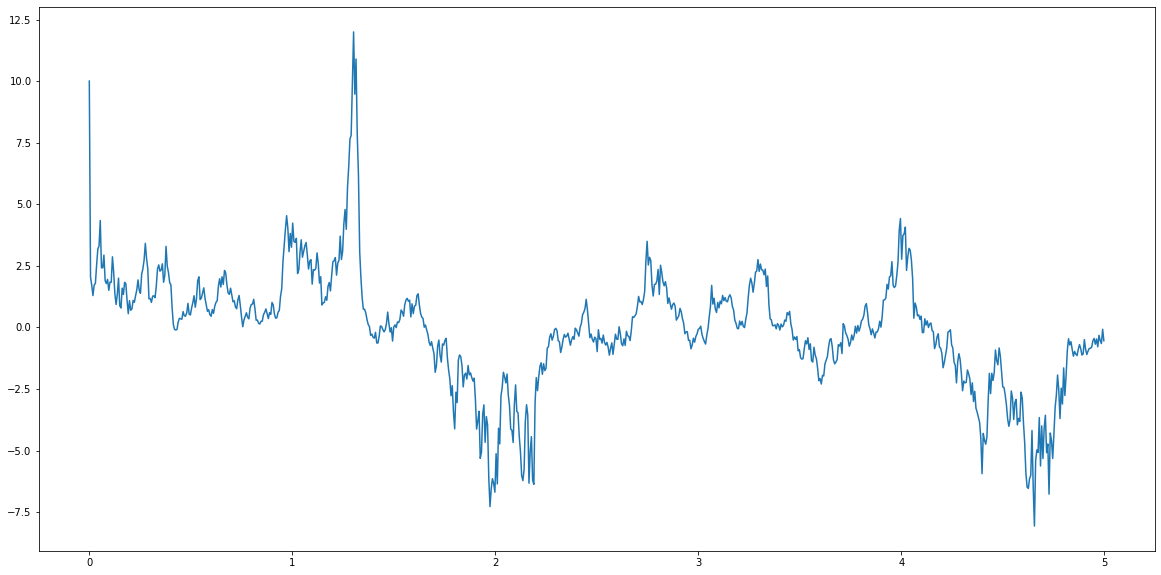
\includegraphics[width=2.95in]{images/4.1/path_4.1.1}}
	\subfigure[样本轨迹2]{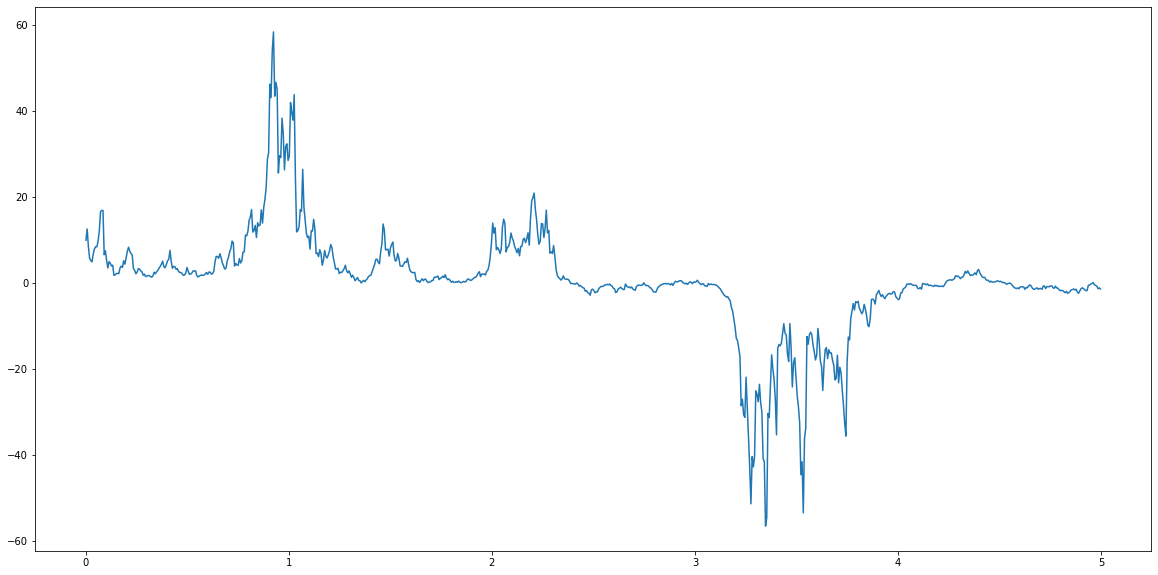
\includegraphics[width=2.95in]{images/4.1/path_4.1.2}}
	\vspace{.2cm}
	\caption{存在稳定解的样本轨道}
	\label{path_4_1}
\end{figure}





\subsection*{例2}
考虑方程
\[
 \md x = bx \md t + \sqrt{2} (1-x^2)\md B_t ,\qquad x\in(-1,1)
\]
其中 $b<0$. 
该随机系统的值域落在$(-1,1)$内.这是因为当 $x \to 1^-$ 或 $x\to (-1)^{+}$ 时,扩散项会收缩到0,而漂移项给予该随机系统一个向着0回归的趋势,同时,任意的样本轨道都是连续的,使得系统无法“跳跃”过 $-1$ 和 $1$ 两个点. 
选取 Lyapunov 函数为 $U(x) =  -\ln(1-x^2)$,
\[
\mL U(x) = 2+2x^2+\frac{2bx^2}{1-x^2},
\]
当 $|x| \to 1^-$ 时,$\mL U(x) \le 3 + 2b U(x)$,从而满足强 Lyapunov 条件. 

\begin{figure}[!htbp]
	\centering 
	\subfigure[T=0.00]{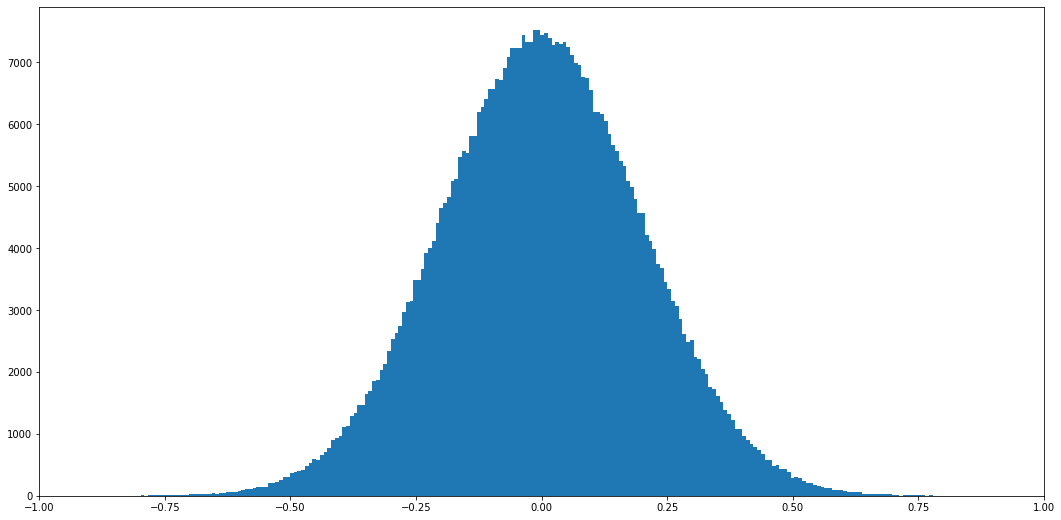
\includegraphics[width=1.45in]{images/4.2/fig_4.2(T=0.00)}}
	\subfigure[T=0.01]{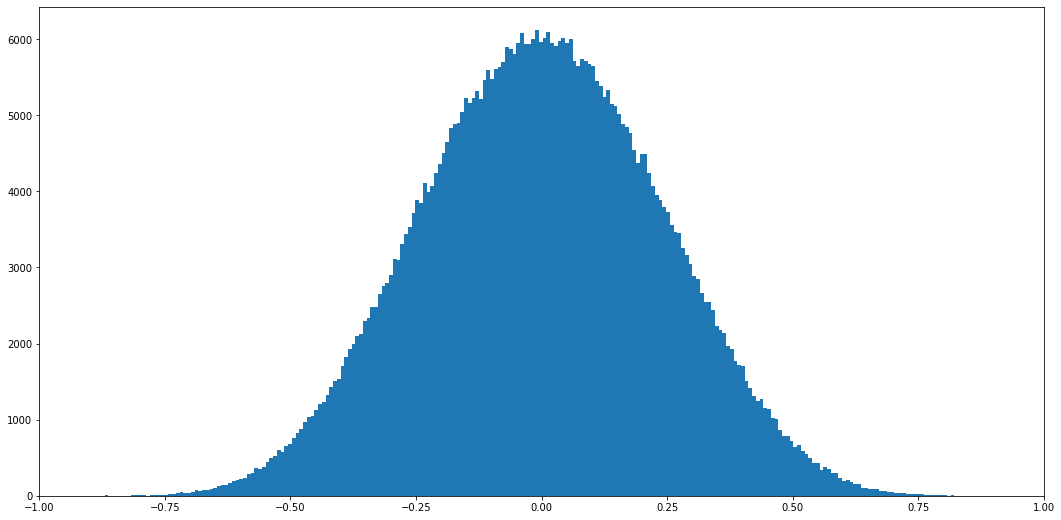
\includegraphics[width=1.45in]{images/4.2/fig_4.2(T=0.01)}}
	\subfigure[T=0.02]{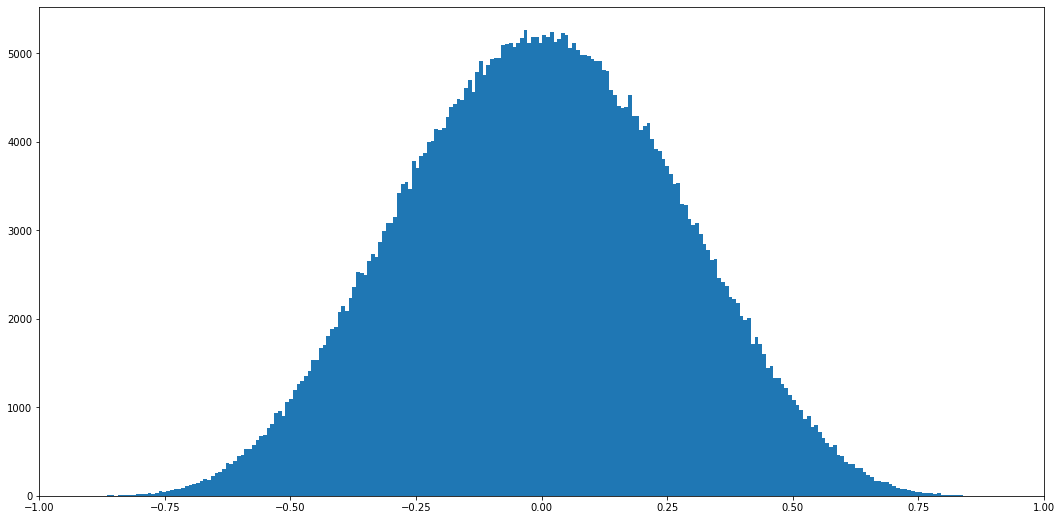
\includegraphics[width=1.45in]{images/4.2/fig_4.2(T=0.02)}}
	\subfigure[T=0.05]{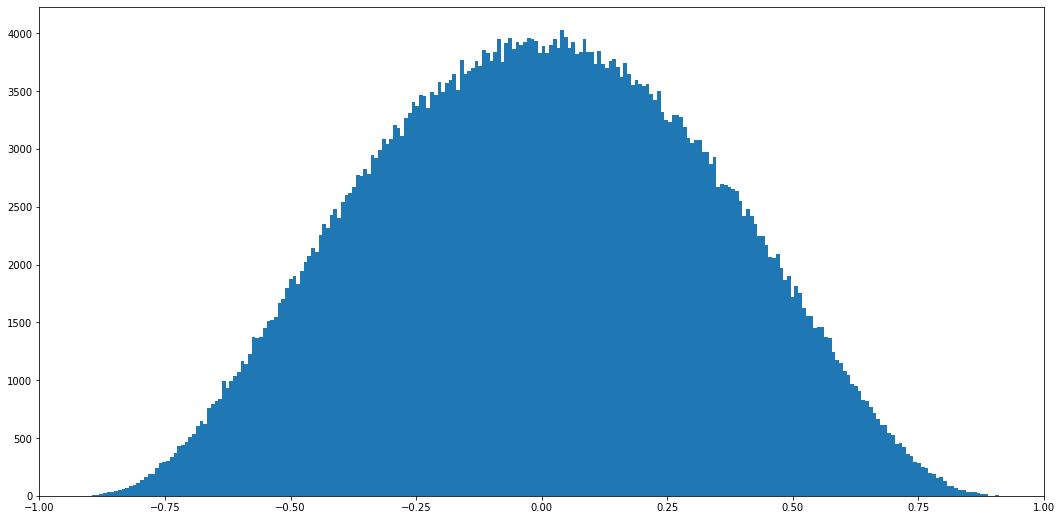
\includegraphics[width=1.45in]{images/4.2/fig_4.2(T=0.05)}}
	\subfigure[T=0.10]{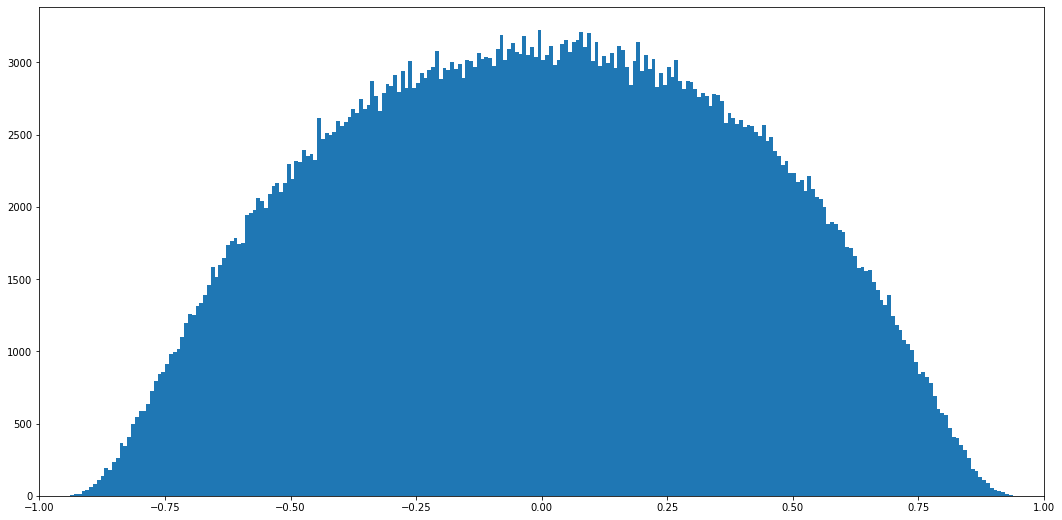
\includegraphics[width=1.45in]{images/4.2/fig_4.2(T=0.10)}}
	\subfigure[T=0.20]{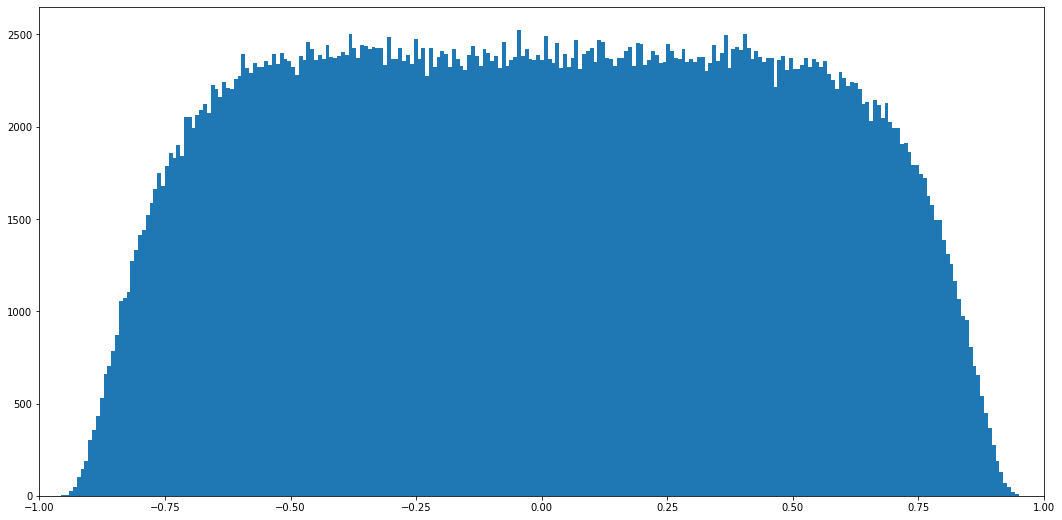
\includegraphics[width=1.45in]{images/4.2/fig_4.2(T=0.20)}}
	\subfigure[T=0.50]{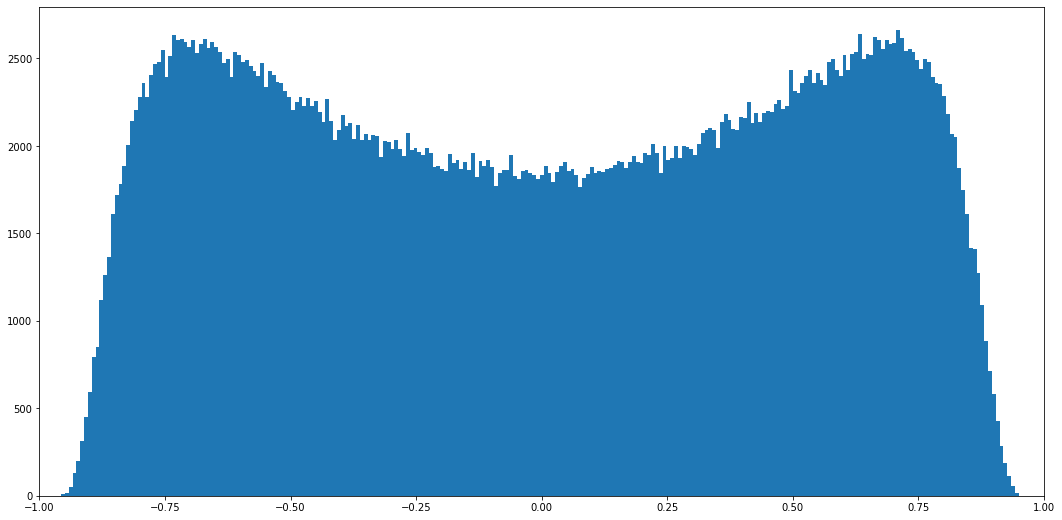
\includegraphics[width=1.45in]{images/4.2/fig_4.2(T=0.50)}}
	\subfigure[T=1.00]{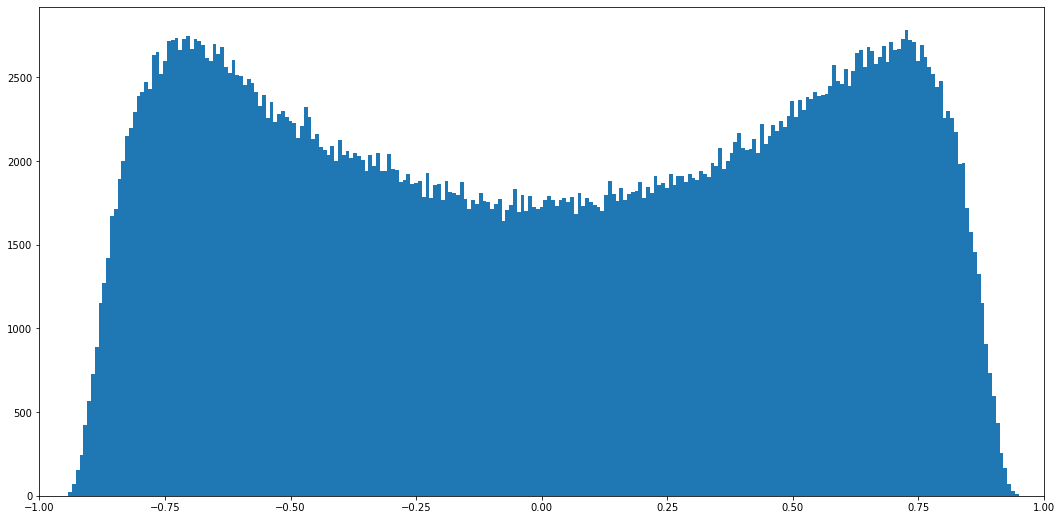
\includegraphics[width=1.45in]{images/4.2/fig_4.2(T=1.00)}}
	\subfigure[T=2.00]{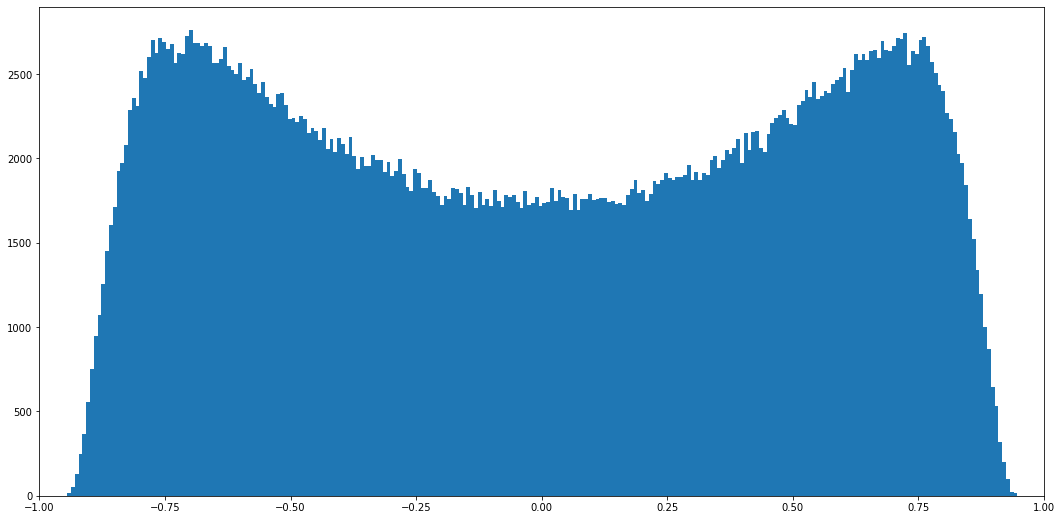
\includegraphics[width=1.45in]{images/4.2/fig_4.2(T=2.00)}}
	%\subfigure[T=4.00]{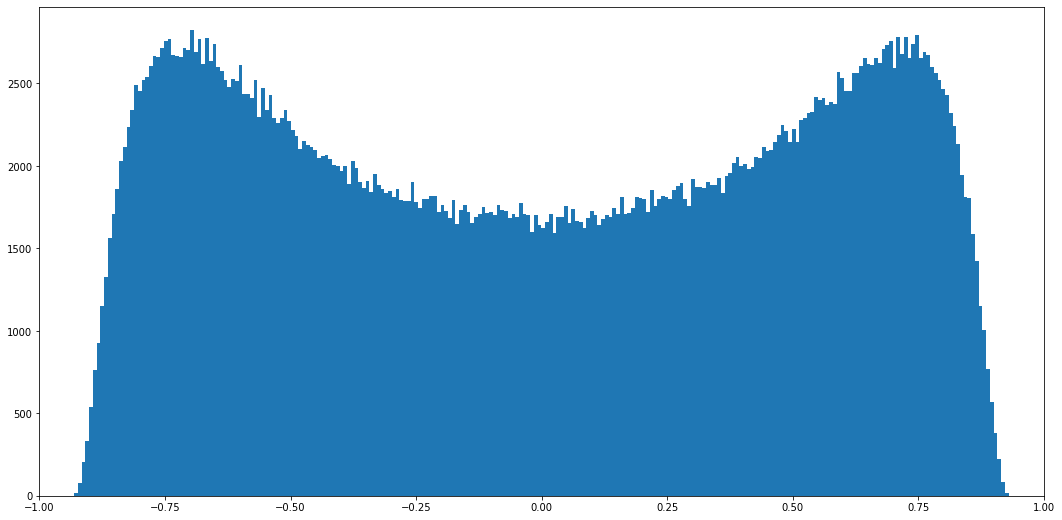
\includegraphics[width=1.45in]{images/4.2/fig_4.2(T=4.00)}}
	\subfigure[T=5.00]{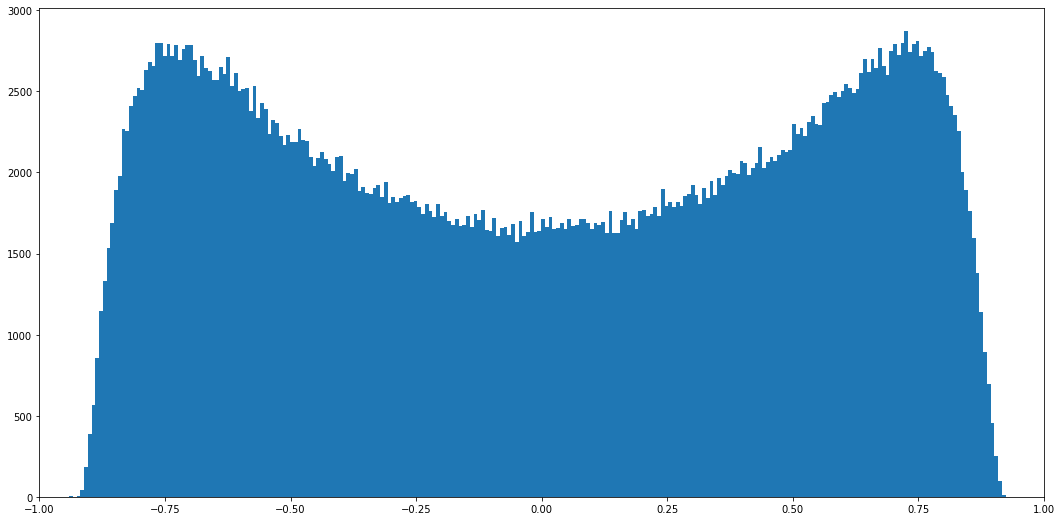
\includegraphics[width=1.45in]{images/4.2/fig_4.2(T=5.00)}}
	%\subfigure[T=8.00]{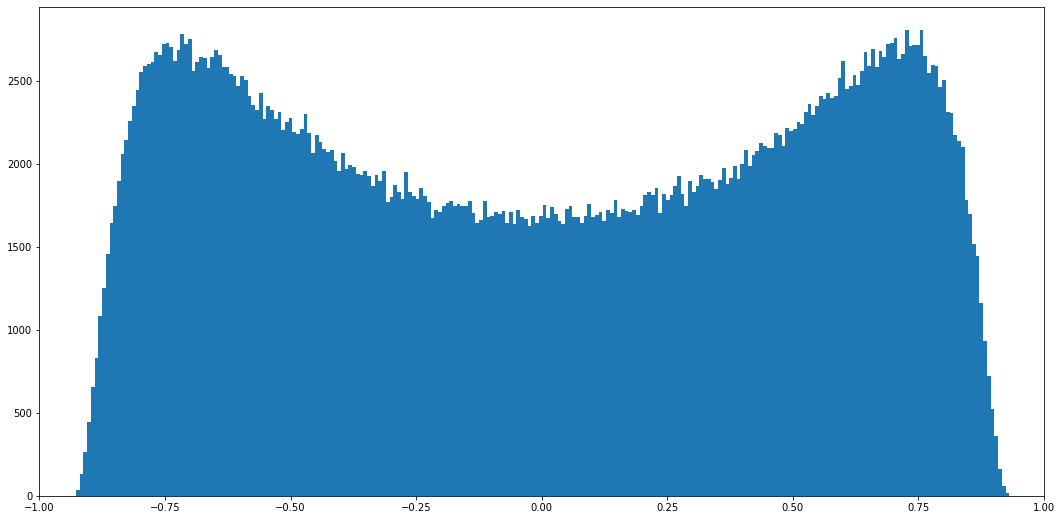
\includegraphics[width=1.45in]{images/4.2/fig_4.2(T=8.00)}}
	\subfigure[T=10.0]{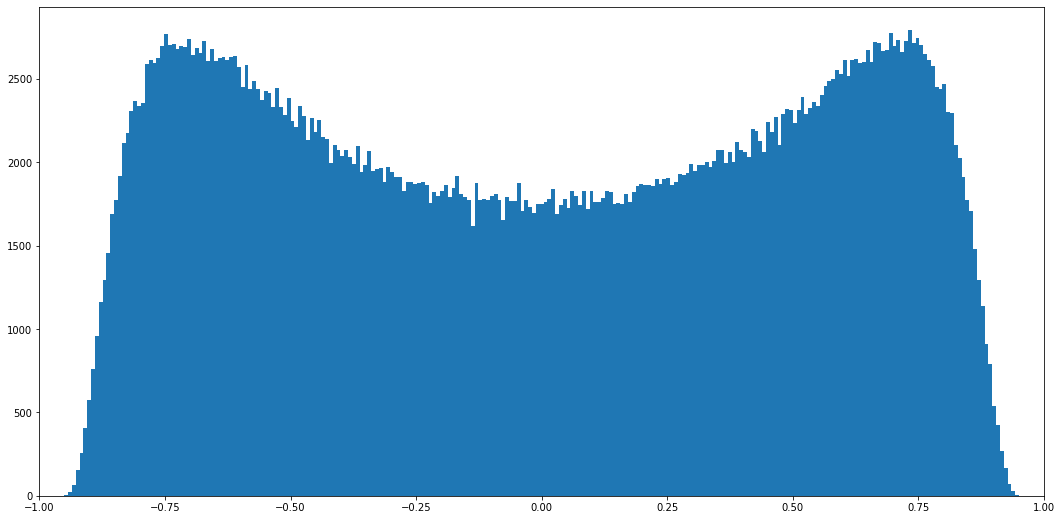
\includegraphics[width=1.45in]{images/4.2/fig_4.2(T=10.0)}}
	\subfigure[T=20.0]{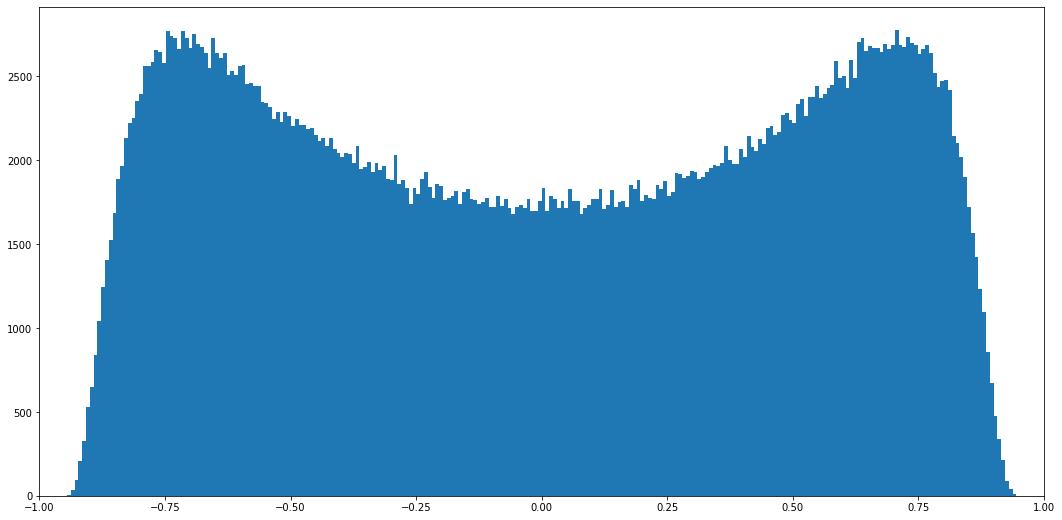
\includegraphics[width=1.45in]{images/4.2/fig_4.2(T=20.0)}}
	\centering
	\vspace{.2cm}
	\caption{稳定解的概率分布(二)}
	\label{measure_4_2}
\end{figure}

数值实验选取初值 $X_0$ 为正态分布 $N(0,0.2)$,并除去落在 $(-1,1)$ 以外的不合理的样本点,模拟结果见图\ref{measure_4_2},可以看出随机系统长时间演化后形成了特定的概率分布. 


\subsection*{例3}
并非所有 SDE 都存在稳定解,如下面的随机微分方程的概率解就会不断扩散,
\[
\md X = \sin(X) \md t + \sqrt{2} \md B_t,\qquad P(X_0 = 0)=1.
\]
\begin{figure}[!htbp]
	\centering 
	\subfigure[T=1]{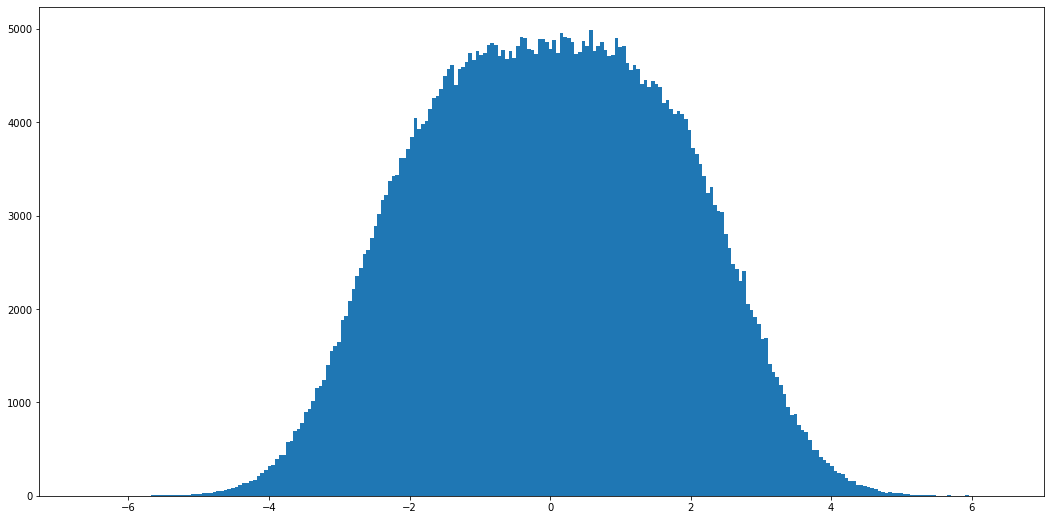
\includegraphics[width=1.45in]{images/4.3/fig_4.3(T=1)}}
	\subfigure[T=5]{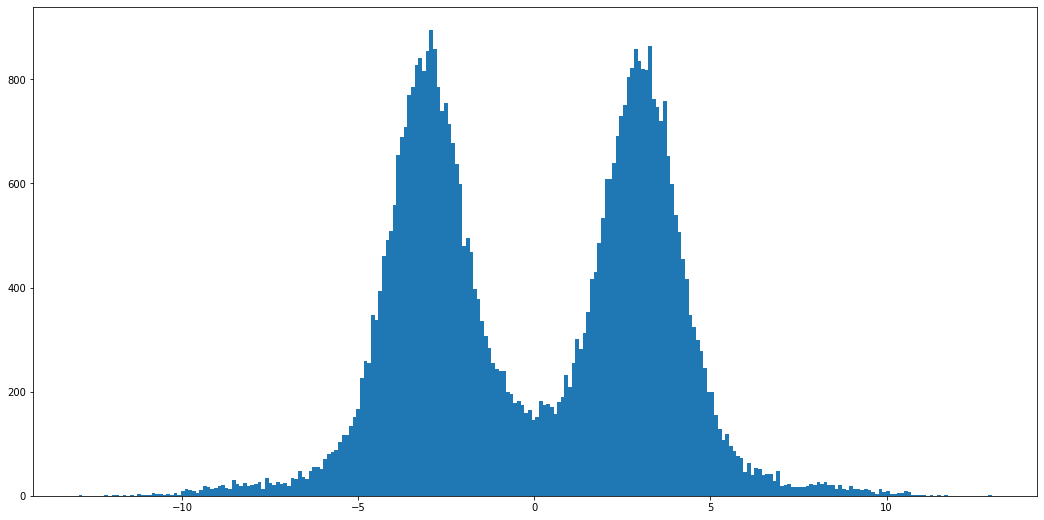
\includegraphics[width=1.45in]{images/4.3/fig_4.3(T=5)}}
	\subfigure[T=10]{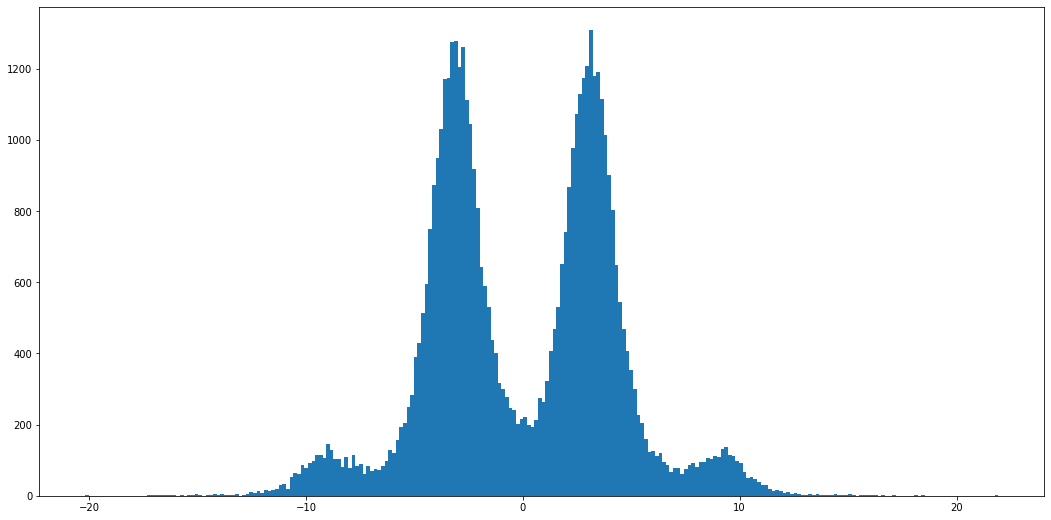
\includegraphics[width=1.45in]{images/4.3/fig_4.3(T=10)}}
	\subfigure[T=50]{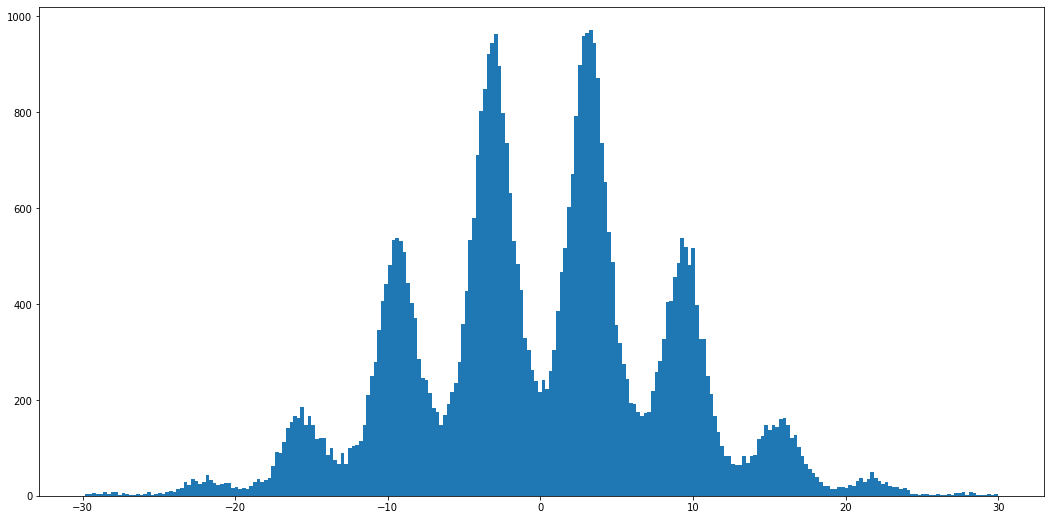
\includegraphics[width=1.45in]{images/4.3/fig_4.3(T=50)}}
	\centering
	\vspace{.2cm}
	\caption{不存在稳定解的概率分布}
	\label{measure_4_3}
\end{figure}
与之前两个可以生成稳定解的例子不同,该例中随机系统的漂移项和扩散项不会互相制约,使得系统达到一个稳定的状态. 
稳定解对应转移方程 $T_{t_0} \mu = \mu$,即稳定解在自治系统作用时间 $t_0$ 后概率分布维持不变,而该系统不存在这样的概率分布. 


\section{稳定解的加速算法}
对于自治随机微分方程,若存在稳定解,考虑初始概率分布 $\mu_0$ 和经过时间 $t$ 之后得到的概率分布为 $\mu_t$,两者具有同样的稳定概率分布 $\mu^*$.也就是说,两个不同的初始概率分布具有一致的稳定解. 
当稳定解唯一时,即算子 $\mL$ 对应的方程的解唯一时,自治随机微分方程在任意初值条件下均能达到稳定解. 现考虑稳定解唯一的情况,本节探讨稳定解的数值算法. 

随机微分方程数值解的模拟很费时间,对于收敛速度慢的随机系统,全程使用较小的步长 $h$ 会使得总计算时长大大增加;而全程使用较大的步长 $h$,则会导致误差较大. 文献\cite{Fokker_Planck}指出,若满足强 Lyapunov 条件,稳定解的收敛速度是甚至指数级的,即:
\[
	\| \mu_t -\mu^* \|_{\operatorname{TV}} \le Ce^{-rt}. 
\]
而 $p$ 阶单步算法导出的概率解 $\tilde \mu_t$ 是失真的. 但只要满足
\[
	\| \tilde{ \mu} _t - \mu_t \|  + \| \mu_t -\mu^* \|  < \| \mu_0 -\mu^* \| ,
\]
则该过程的演化仍然是有价值的. 这是因为失真的的概率解 $\tilde\mu_t$ 并不会影响最终的稳定解. 
注意到 $\| \tilde \mu_t - \mu_t \| $ 的精度是 $O(h^p)$,而计算时间是 $O(\frac1h)$. 因此设计如下数值算法:

\begin{algorithm}[!htbp]
	\caption{稳定解的加速算法}%算法名字
	\LinesNumbered %要求显示行号
	\KwIn{SDE 系统,误差界$\varepsilon$,样本轨道数$N$}%输入参数
	%\KwOut{output result}%输出
	$X = \mathcal N(0,1,N),\quad h=0.1,\quad \rm{time} = 0$\;
	\For{\rm{i in \{0,1,2,…,10\}}}{
		h = h / 2 \;
		M = pow(2,i)\;
		\For{\rm{j in \{0,1,2,…,M\}}}{
			time = time + h\;
			newX = scheme(X,h)\;
			\If{$\|\rm{sort(newX)-sort(X)}\| < \varepsilon$}{
				break\;
			}\Else{
				newX = X\;
			}
		}
	}
\end{algorithm}

当稳定解唯一时,稳定解的初值无关性带来极大的好处,算法运行初期引入的误差是不会影响最终的解,但使用较大的步长 $h$ 可以使程序快速收敛到稳定解附近,而后续过程将 $h$ 取的较小,又可以使得精度相较普通方法更高. 


但如果稳定解不唯一,数值实验表明该算法不一定会收敛. 本文下一章节针对一类稳定解存在但不唯一的随机系统,提出了相应的求解稳定解的加速算法. 














 % 解的长时间特性
  % !Te\overline  encoding = UTF-8
\chapter{带守恒量的SDE的数值解法}\label{chap5}
本节考虑的是带守恒量的自治随机微分方程的数值解法,因此不能只保障算法的精度,还要求数值算法能维持系统的守恒量不变. 本节处理 \ito 型自治随机微分方程(\ref{SODE}):
\begin{equation}\label{eq5.1}
	\begin{aligned} 
	&\md X(t) = b(X) \md t + \sigma (X) \md B_t ,\qquad 0 \le t\le  T,\\
	&X(0) = X_0
	\end{aligned}
\end{equation}
首先将其处理成等价的 Stratonovich 型自治随机偏微分方程:
\begin{equation}\label{eq5.2}
	\begin{aligned} 
	&\md X(t) = f(X)\md t + g(X) \circ \md B_t,\qquad  0 \le t \le T,\\
	&X(0) = X_0
	\end{aligned}
\end{equation}
其中 
\begin{equation}\label{eq5.3}
\left\{
\begin{aligned}
	f(X) &= b(X) - \frac12 \frac{\partial \sigma(X)}{\partial X} \sigma(X),\\\ g(x) &= \sigma(X).
\end{aligned}
\right.
\end{equation}
这两种表述形式的区别在于积分形式下,分割取点的位置不同,见本文第2节关于随机积分的论述. 
与之前一致,要保证强解的存在性和唯一性,需要有Lipschitz条件和线性增长条件:
\begin{equation}\label{eq5.4}
\begin{aligned}
	&\| f(x) - f(y)\| + \|g(x)-g(y)\| \le K_1 \| y-x\|,\\
	&\| f(x)\| ^2 + \| g(x) \| \le K_2 (1+\|x\|^2).
\end{aligned}
\end{equation}



\section{SG 形式与对称离散梯度}
对于 Stratonovich 型随机偏微分方程(\ref{eq5.2}),考虑随机系统存在如下的守恒量,
\begin{definition}[守恒量]
	称可微标量函数 $I(x)$ 为SDE(\ref{eq5.2}) 的守恒量,若其满足
	\begin{equation}\label{eq5.5}
		\nabla I^T(x) f(x) = 0,\qquad \nabla I^T(x) g(x) = 0.
	\end{equation}
\end{definition}
守恒量反映系统固有的某种“能量”属性. 构造方程(\ref{eq5.4})的等价SG形式:
\begin{equation}\label{eq_SG}
	\md X = S(X) \nabla I(X) \md t +  T(X) \nabla I(X) \circ \md B_t,
\end{equation}
当守恒量存在时,必定存在这样的函数 $S,T$,且为反对称矩阵. 如
\begin{equation}
	S(x)=\frac{f(x) a(x)^{T}-a(x) f(x)^{T}}{a(x)^{T} \nabla I(x)}, \quad T(x)=\frac{g(x) b(x)^{T}-b(x) g(x)^{T}}{b(x)^{T} \nabla I(x)}
\end{equation}
这边的函数 $a,b$ 是任意选取的,只要满足 $a(x)^T \nabla I(x)\neq 0,\quad b(x)^T \nabla I(x) \neq 0 $ 即可. 由于(\ref{eq5.5})不难验证该构造是合理的. 接下来,需要引入对 $\Delta I$ 的估计.
\begin{definition}
	称 $\overline{\nabla} I(x,\overline{ x })$ 为 $x$ 和 $\overline x$ 的离散梯度,若 $\overline \nabla I(x,\overline x) ^ T (x - \overline x) = I(x) - I(\overline x)$  且 $\overline \nabla I(x,x) = \nabla I(x)$. 进一步地,若 $\overline \nabla I(x,\overline x) = \overline \nabla I(\overline x,x)$,则称之为对称离散梯度.
\end{definition}

对称离散梯度的选择并不是唯一的,且对称的性质是必要的,这是保持数值格式具有一阶精度的关键. 可以按照下面方式构造对称梯度:$ \overline \nabla I(x,\overline x) = \frac12( \overline \nabla_1 I(x,\overline x) +  \overline \nabla_1 I(\overline x,x)  ) $,其中
\[
\overline{\nabla}_1 I(x, \overline{x}):=
\left(\begin{array}{c}
\frac{I\left(\overline{x}^{1}, x^{2}, x^{3}, \ldots, x^{d}\right)-I\left(x^{1}, x^{2}, x^{3}, \ldots, x^{d}\right)}{\overline{x}^{1}-x^{1}} \\
\frac{I\left(\overline{x}^{1}, \overline{x}^{2}, x^{3}, \ldots, x^{d}\right)-I\left(\overline{x}^{1}, x^2, x^3, \ldots, x^d\right)}{\overline{x}^{2}-x^{2}} \\
\vdots \\
\frac{I\left(\overline{x}^{1}, \overline{x}^2, \overline{x}^2, \ldots, \overline{x}^{d}\right)-I\left(\overline{x}^1, \overline{x}^2, \ldots, \overline{x}^{d-1}, x^{d}\right)}{\overline{x}^d-x^d}
\end{array}\right) .
\]
代入即可验证 $\overline \nabla I$ 满足对称离散梯度的要求. 





\section{直接离散格式与间接离散方法}
现在给出对于 Stratonovich 型随机偏微分方程(\ref{eq5.2})的保持守恒量的直接离散梯度格式. 将时间区间离散成 $N$ 份,步长 $h = \frac TN$,$t_n= nh \ (n=0,1,2,\cdots,N)$. 给出数值格式
\begin{equation}\label{scheme_discrete_1}
	\overline{ x }_{n+1} = \overline x_n + S(\overline{ x }_n) \overline \nabla I(\overline{ x }_n,\overline{ x }_{n+1}) h + T\left( \frac{\overline{ x }_n + \overline{ x }_{n+1}}{2} \right)\overline \nabla I(\overline{ x }_n,\overline{ x }_{n+1}) \Delta_B
\end{equation}
$\{\overline x_n\}_{n=0}^N$ 为 SDE 在直接离散梯度格式下的近似解. 

\begin{theorem}
	若 $S,T,I$ 二阶矩有限且 $S,T,I \in C^2(\R^d)$ 具有一致有界的导数,则数值格式\ref{scheme_discrete_1}满足以下性质:
	\begin{enumerate}
		\item 格式保持守恒量,即 $I(\overline x_{n+1}) = \overline x_n$.
		\item 格式具有一阶整体均方误差,即
			\[
			(E \| x(t_n) - \overline x_n\| ^2 )^{\frac12} = O(h). 
			\]
	\end{enumerate}
\end{theorem}
\begin{proof}
	由 (\ref{scheme_discrete_1}) 与 $S,T$ 为反对称的矩阵,有
	\[
	\begin{aligned}
	I(\overline x_{n+1})& - I(\overline x_n) = \overline\nabla I(\overline x_{n+1} , \overline x_n)(\overline{ x }_{n+1} -\overline x_n ) \\
	&= \overline\nabla I(\overline x_{n+1} , \overline x_n) S(\overline x_n) \overline\nabla I(\overline x_{n+1} , \overline x_n) h + 
	\overline\nabla I(\overline x_{n+1} , \overline x_n) T(\frac{(\overline x_{n+1} + \overline x_n)}{2}) \overline\nabla I(\overline x_{n+1} , \overline x_n) \Delta_B = 0.
	\end{aligned}
	\]
	下证该数值格式的精度. 由于定理\ref{thm_3.1},只需证该格式的局部误差满足
	\begin{equation}\label{eq5.9}
	\| E(\overline x_{n+1} -  x_{t,\overline x_n}(t+h) ) \| = O(h^2),\qquad
	\left( E\| \overline x_{n+1} - x_{t,\overline x_n}(t+h) \| ^2 \right) ^{\frac12} = O(h^{\frac32}). 
	\end{equation}
	而 Milstein 格式同样具有1阶整体误差. 在Stratonovich格式下,表述为:
	\[
	\tilde x_{n+1} = \overline x_n+S(x)\nabla I(\overline x_n) h + T(\overline x_n) \nabla I(\overline x_n) \Delta_B + \frac12\left( \frac{\partial (T\nabla I)}{\partial x}  T \nabla I\right) h. 
	\]
	且有:
	\[
	\| E(\tilde x_{n+1} - x_{t,\overline x_n}(t+h)) \| = O(h^2),\qquad
	\left( E\| \tilde x_{n+1} - x_{t,\overline x_n}(t+h) )\| ^2 \right) ^{\frac12} = O(h^{\frac32}). 
	\]
	注意到该格式是显格式,将其分量函数展开,为
	\begin{equation}
	\begin{aligned} 
		\tilde x^k_{n+1} = \overline x_n^k& + \sum_{i=1}^d (S^{ki} \partial _i I)h +\sum_{i=1}^d (T^{ki}\partial _i I) \Delta_B  \\
		&+\frac12 \sum_{i=1}^d \sum_{j=1}^d (\partial_j T^{ki}\partial_iI + T^{ki} \partial _{ij}I) \left( \sum_{l=1}^d T^{jl}\partial l I \right) h.
	\end{aligned}
	\end{equation}
	
	另一方面,对 $\overline \nabla I(\overline x_n,\overline x_{n+1})$ 和 $T(\frac{\overline x_n+\overline x_{n+1}}{2})$ 在 $\overline x_n$ 处做 Taylor 展开,令 $\Delta^j = \overline x_{n+1}^j - \overline x_{n}^j$,有
	\[ 
	\begin{aligned}
	&\overline T_{kj} := T^{ki} \left(\overline x_n + \frac{\overline x_{n+1}-\overline x_{n}}{2}\right) =  T^{ki}(\overline x_n) + \frac12\sum_{j=1}^d \partial _j T^{ki}(\overline x_n) \Delta^j + R_T\\
	&\overline \nabla I^k: = \overline \nabla I^k\left(\frac{\overline x_n+\overline x_{n+1}}{2}\right) =
	\partial_{k} I(\overline x_n)+\frac{1}{2} \sum_{j=1}^{d} \partial_{k j} I(\overline x_n) \Delta^{j}+\frac{1}{2} R_{I}
	\end{aligned}
	\]
	这里 $R_T$ 与 $R_I$ 均为误差项 $\Delta ^ j$ 的高阶项.  
	
	
	将 Taylor 展开式带入直接离散梯度格式,再与 Milstein 格式的展开式相减,得残差项
	\[
	\begin{aligned}
	R^k := \tilde{x}^k_{n+1} -\overline x_{n+1}^k  &=\sum_{i=1}^{d} S^{k i}\left(\overline {\nabla} I^{i}-\partial_{i} I\right) h+\frac{1}{2} \sum_{i=1}^{d} T^{k i} R_{I} \Delta_B+\frac{1}{2} \sum_{i=1}^{d} \sum_{j=1}^{d} \partial_{j} T^{k i} \Delta^{j}\left(\overline{\nabla} I^{i}-\partial_{i} I\right) \Delta_B \\
	&+\sum_{i=1}^{d} R_{T} \overline{\nabla} I^{i} \Delta _B+\frac{1}{2} \sum_{i=1}^{d} \sum_{j=1}^{d}\left(\partial_{j} T^{k i} \partial_{i} I+T^{k i} \partial_{i j} I\right)\left(\Delta^{j}-\sum_{l=1}^{d} T^{j l} \partial_{l} I \Delta _B\right) \Delta _B
	\end{aligned}
	\]
	利用 Brown 运动的性质: $E B_t = 0,\text{~} EB_t^2 = h,\text{~} EB_t^3=0,\text{~} EB_t^4 = 3h^2\cdots$ 可得:
	\[
	|E\Delta^j| = O(h),\quad |E(\Delta^j)^2|^{1/2} = O(h^{1/2}),\qquad j=1,2,\cdots,d.
	\]
	从而有
	\[
	\tilde{x}^k_{n+1} -\overline x_{n+1}^k = C_1 h^2 + C_2h\Delta_B + O(h^2\Delta_B).
	\]
	因此有
	\[
		\left| E(\tilde{x}^k_{n+1} -\overline x_{n+1}^k) \right| = O(h^2),\quad
		\left( E(\tilde{x}^k_{n+1} -\overline x_{n+1}^k)^2 \right)^{\frac12} = O(h^{\frac32}).
	\]
	由 Milstein 格式的局部误差估计式和 Minkowski 不等式,得(\ref{eq5.9})成立. 
\end{proof}

在 Taylor 展开的处理过程中,关键之处在于 $\overline{\nabla}I(\overline{ x }_n , \overline{ x }_{n+1})$ 和 $T(\frac{\overline{ x }_n + \overline{ x }_{n+1}}2)$,而对 $S$ 并没有太高的要求,因此下面的直接离散梯度格式也保持守恒量并具有一阶精度. 
\begin{equation}\label{scheme_discrete_2}
\hat{ x }_{n+1} = \hat x_n + S\left(\frac{\hat x_n+\hat x_{n+1}}{2}\right) \overline \nabla I(\hat{ x }_n,\hat{ x }_{n+1}) h + T\left( \frac{\hat{ x }_n + \hat{ x }_{n+1}}{2} \right)\overline \nabla I(\hat{ x }_n,\hat{ x }_{n+1}) \Delta_B
\end{equation}

将数值格式(\ref{scheme_discrete_1})和(\ref{scheme_discrete_2})称为直接离散梯度. 除此之外,SG形式的特殊性,使得还可以构造另一种称为间接离散梯度的方法. 重述(\ref{eq_SG}) 为
\[
\md X = V_0(X) \md t + V_1(X) \circ \md B_t,
\]
其中漂移项 $V_0 = \sum ^d_{i,j=1} S^{ij} \frac{\partial I}{\partial x^j}\frac{\partial}{\partial x^i}$,扩散项 $V_1 = \sum ^d_{i,j=1} T^{ij} \frac{\partial I}{\partial x^j}\frac{\partial}{\partial x^i}$. 注意到 $S,T$ 是反对称矩阵,因此有
\[
V_{0}^{i j}=S^{i j} \frac{\partial I}{\partial y^{j}} \frac{\partial}{\partial y^{i}}+S^{j i} \frac{\partial I}{\partial y^{i}} \frac{\partial}{\partial y^{j}}, V_{1}^{i j}=T^{i j} \frac{\partial I}{\partial y^{j}} \frac{\partial}{\partial y^{i}}+T^{j i} \frac{\partial I}{\partial y^{i}} \frac{\partial}{\partial y^{j}}, 1 \leq i<j \leq d
\]
于是原SG系统可以拆分为 $\frac{d(d-1)}{2}$ 个子系统:
\[
d x_{i j}=V_{0}^{i j}(x_{i j}) \md t+V_{1}^{i j}(x_{i j}) \circ \md \Delta_B, \quad 1 \leq i<j \leq d.
\]
对每个子系统都使用直接离散梯度方法操作,每个子系统的处理用算子 $Y_{i,j}$ 表示,故
\begin{equation}\label{scheme_discrete_3}
	\overline x_{n+1} = Y_{1,2}\circ Y_{1,3}\circ \cdots \circ Y_{d-2,d}\circ Y_{d-1,d} \circ \overline x_n. 
\end{equation}
由于每步都是直接离散梯度方法,因此间接离散梯度依然保持守恒量不变. 在另一些文献中,将间接离散梯度方法设计为:
\[
\begin{aligned}
\overline x_{n+1}=& \overline {Y}_{1,2}(\frac12) \circ \overline {Y}_{1,3}(\frac12) \circ \cdots \circ \overline {Y}_{d-2, d}(\frac12) \circ \overline {Y}_{d-1, d}(1) \circ \overline {Y}_{d-2, d}(\frac12) \circ \\
& \cdots \circ \overline {Y}_{1,3}(\frac12)\circ \overline {Y}_{1,2}(\frac12)\circ \overline x_n
\end{aligned}
\]
这里 $\overline Y_{i,j}(\lambda)$ 指子系统前进 $\lambda h$ 的步长. 
带守恒量的自治随机微分方程的间接离散梯度方法的算法如下:


\begin{algorithm}[!htbp]
	\caption{间接离散方法求解带守恒量的自治随机微分方程}%算法名字
	\LinesNumbered %要求显示行号
	\KwIn{SDE 系统}%输入参数
	%\KwOut{output result}%输出
	将 \ito 型随机微分方程(\ref{eq5.1})处理成 Stratonovich 型随机微分方程(\ref{eq5.2})\;
	寻找合适的反对称矩阵 $S,T$,将微分方程处理成 SG形式\ref{eq_SG}\;
	构造格式的对称离散梯度 $\overline \nabla I$\;
	拆分成 $\frac{d(d-1)}{2}$ 个子系统\; 
	\For{\rm{i in \{1,2,…,N\}}}{
		\For{\rm{a in \{0,1,…,d-1\}}}{
			\For{\rm{b in \{a+1,a+2,…,d\}}}{
				$X = Y_{a,b} (X)$ \;
			}
		}
	}
\end{algorithm}


\newpage



\section{投射方法}
另一种保持守恒量的算法则直观得多. 对一些问题,已经有1.5阶甚至更高阶的单步算法,尽管往往算法并不直接保证随机系统的守恒量,但可以在每次数值迭代之后,将其“拉”回到守恒量对应的流形上去. 现有算法如下:


\begin{figure}[!htbp]
	\centering 
	\subfigure{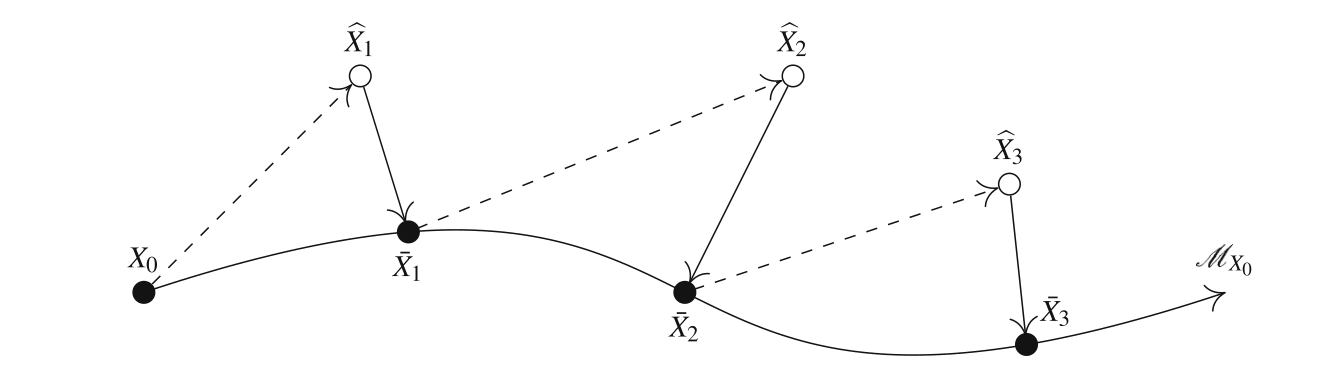
\includegraphics[width=4.95in]{images/project.png}}
	\vspace{.2cm}
	\caption{投射方法}
	\label{fig.5}
\end{figure}

有 $X(t) \in \mathscr M_{X_0} := \{ x\in\R^d : I(x) = I(X_0) \},\quad t\in[0,T],\quad \rm{a.s.}$.



\begin{algorithm}[!htbp]
	\caption{投射方法求解带守恒量的自治随机微分方程}%算法名字
	\LinesNumbered %要求显示行号
	\KwIn{SDE 系统、单步方法的数值格式}%输入参数
	%\KwOut{output result}%输出
	%将 \ito 型随机微分方程处理成 Stratonovich 型随机微分方程\;
	%寻找合适的反对称矩阵 $S,T$,将微分方程处理成 $SG$形式\;
	%构造格式的对称离散梯度 $\overline \nabla I$\;
	%拆分成 $\frac{d(d-1)}{2}$ 个子系统\; 
	\For{\rm{i in \{1,2,…,N\}}}{
		计算单步方法的结果 $\overline X_{t,x}$\;
		计算梯度方向$\Phi \in \R^d$\;
		计算步长$\lambda$\;
		更新守恒解$\widehat X_{t,x} = \overline X_{t,x} + \lambda\Phi$\;
	}
\end{algorithm}


该算法存在两个问题,无法确定投射方向 $\Phi$ 和 $\lambda$ 可能无解. 关于第一个问题,可以用前一个迭代点的 $\overline X$ 的法方向作为投射的梯度方向 $\Phi$,当步长 $h$ 较小且 $\mathscr M_{X_0}$ 较平缓时,该算法的处理是可行的. 但当守恒量流形维度小于 $d-1$ 时,可能无法投射到守恒量所在流形上,导致 $\lambda$ 无解. 

对此,本文提出按照 $L^2$ 距离最短的方式选取投射点. 即如下约束优化问题:
\begin{equation}
	\begin{aligned}
	\begin{aligned}
	&\min _ {\overline X \in \R^d} \frac12 \| \overline X - \widehat X\|_2,\\
	&\qquad \rm{s.t.}\qquad  	I(\overline X) = I(X_0)
	\end{aligned}
	\end{aligned} 
\end{equation}
考虑 SDE 带有 $r$ 个守恒量 $I_1,I_2,\cdots,I_r$,则对应的拉格朗日乘子函数为:
\[
L(x_1,x_2,\cdots ,x_d,\lambda_1,\cdots,\lambda_r) = \frac12 \sum _{i=1}^{d} (x_i-\widehat X_i)^2 + \sum_{i=1}^r \lambda_i( I_i(x) - I_i(\widehat X)). 
\]
分别关于 $d$ 个变量和 $r$ 个乘子参数求导,得 $d+r$ 个方程,导入非线性方程求解器,即可得到 $L^2$ 距离最近意义下的投射点. 非线性方程求解器的迭代初始点设置为 $\widehat X$,能很快收敛到 $\overline X$. 
相对于原方法,改进方法投射点更合理,不需要在法空间中确定具体的投射方向,且算法很容易实现. 


\section{带守恒量问题的稳定解}
本节之前部分讨论的均为保持单一样本轨道的守恒量,现考虑随机系统的稳定解. 对于存在稳定解的带守恒量的自治随机微分方程,不同的初值设置下,守恒量初值是可以不同的,因而对应的稳定解也不唯一. 根据守恒量可以对稳定解进行分类. 

由于稳定解不唯一,仅考虑精度的数值格式很可能无法收敛到相应初值下的稳定解,本文提出使用保守恒量的数值格式可以得到带守恒量的问题的稳定解. 数值实验中,对于一个守恒量为 $\frac12(x_1^2+x_2^2)$ 的随机系统进行数值模型,有如下结果:


\begin{figure}[!htbp]
	\centering 
	\subfigure[$x_1$的稳定解]{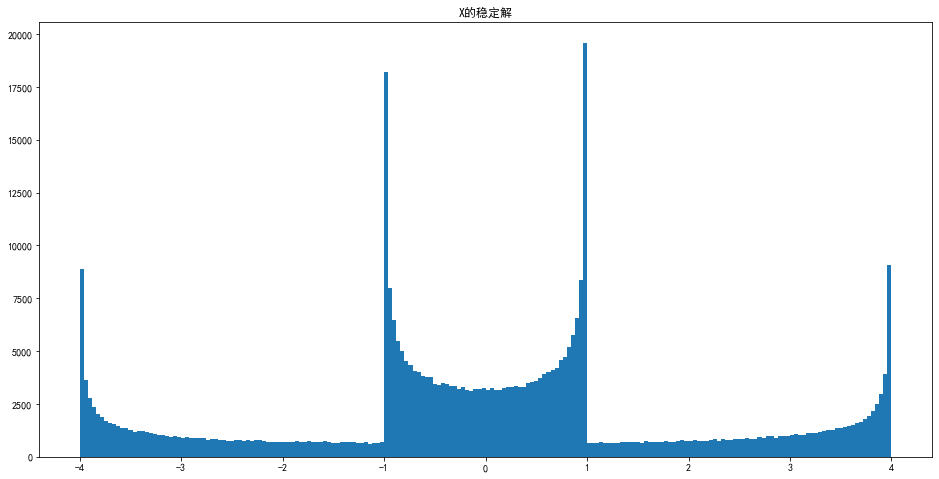
\includegraphics[width=2.95in]{images/5.4/1-x.png}}
	\subfigure[$x_2$的稳定解]{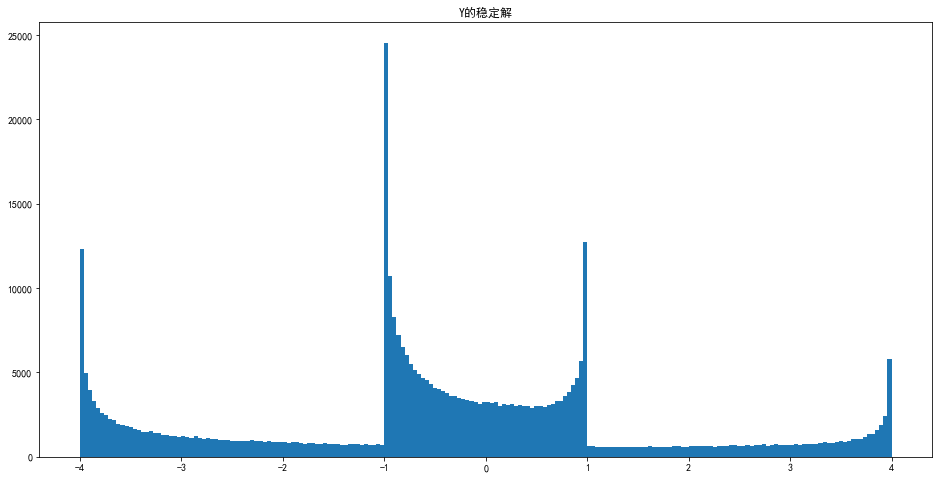
\includegraphics[width=2.95in]{images/5.4/1-y.png}}
	\vspace{.2cm}
	\caption{初值分布为两点分布下的稳定解}
	\label{fig.5.2}
\end{figure}

\begin{figure}[!htbp]
	\centering 
	\subfigure[$x_1$的稳定解]{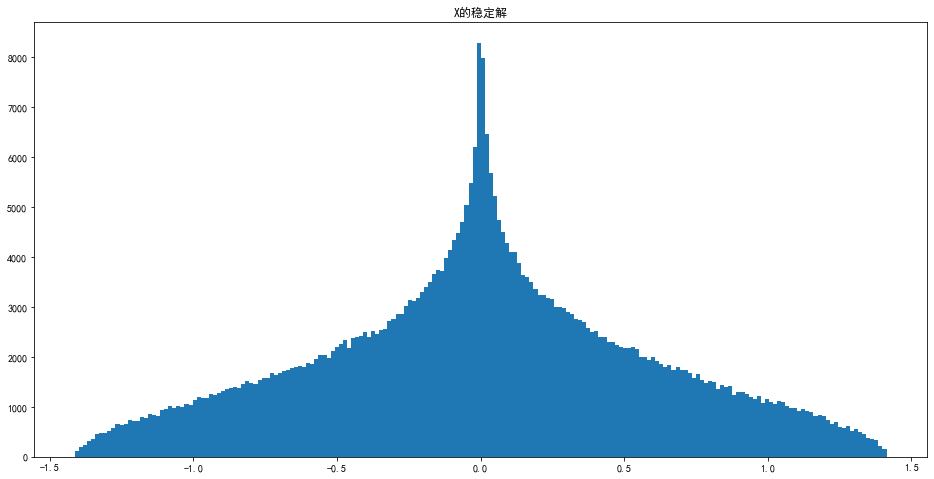
\includegraphics[width=2.95in]{images/5.4/2-x.png}}
	\subfigure[$x_2$的稳定解]{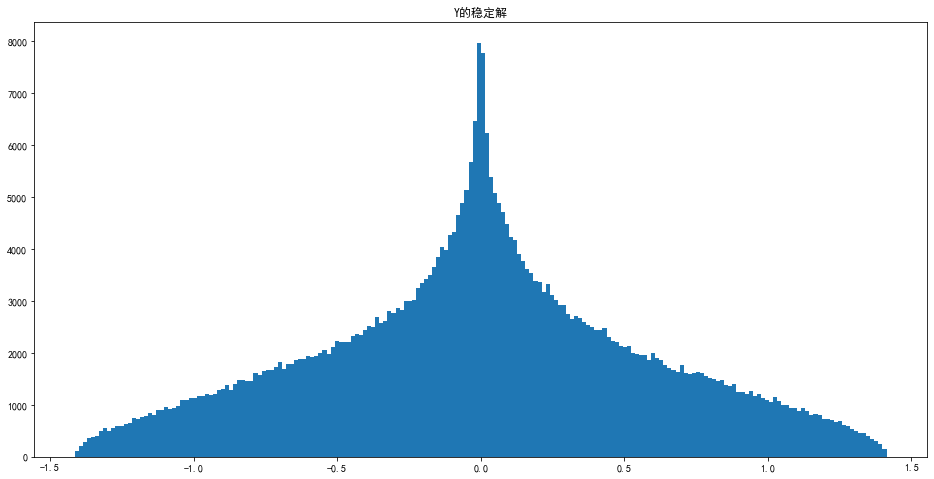
\includegraphics[width=2.95in]{images/5.4/2-y.png}}
	\vspace{.2cm}
	\caption{初值分布为均匀分布的稳定解}
	\label{fig.5.3}
\end{figure}

图\ref{fig.5.2}的初值分布为 $P((x_1,x_2) = (0,1) ) = \frac12$,$P((x_1,x_2) = (0,4) ) = \frac12$. 图\ref{fig.5.2}的初值分布 $x_1=x_2$ 服从分布 $U(0,1]$,考虑的方程均为二维随机 Kubo oscillator 方程. 

本文将带守恒量的自治随机微分方程的稳定解的加速算法总结为:
\begin{algorithm}[!htbp]
	\caption{带守恒量的自治随机微分方程的稳定解的加速算法}%算法名字
	\LinesNumbered %要求显示行号
	\KwIn{SDE 系统,误差界$\varepsilon$,样本轨道数$N$}%输入参数
	%\KwOut{output result}%输出
	$X = \mathcal N(0,1,N),\quad h=0.1,\quad \rm{time} = 0$\;
	\For{\rm{i in \{0,1,2,…,10\}}}{
		h = h / 2 \;
		M = pow(2,i)\;
		\For{\rm{j in \{0,1,2,…,M\}}}{
			time = time + h\;
			newX = scheme(X,h) \# 单步方法  \;
			newX = project(X,$I_1,\cdots,I_r$) \# 投射操作\; 
			\If{$\|\rm{sort(newX)-sort(X)}\| < \varepsilon$}{
				break\;
			}\Else{
				newX = X\;
			}
		}
	}
\end{algorithm}

根据实验,本文推测通过限制守恒量的方式,离散算法的稳定解是收敛的. 




 % 带守恒量的SDE的数值解法
  % !TeX encoding = UTF-8
\chapter{数值实验}\label{chap6}

\section{经典数值格式收敛阶的验证}
几何Brown运动 $\md X(t) = bX(t) \md t+\sigma X(t)\md B_t$ 的精确解是已知的,且仅与随机项的起点与终点有关,
\[
X_t = X_0 \exp\left[ (b+\frac12\sigma^2)t + \sigma B_t \right]
\]
而不需要知道 $B_t$ 具体的样本轨道形态. 
为了防止 $X_t$ 的值随时间指数增长,选择参数 $(b,\sigma) = (-2,2)$. 
利用该方程验证经典的格式的精度,分别测试误差的期望和方差,结果如下图\ref{fig.6.1}:

\begin{figure}[!htbp]
	\centering 
	\subfigure[误差的期望]{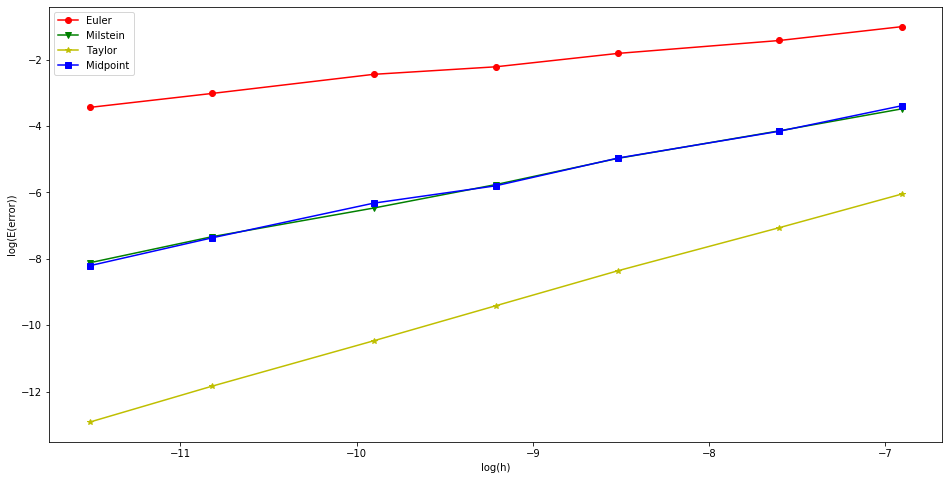
\includegraphics[width=2.95in]{images/6.1.png}}
	\subfigure[误差的方差]{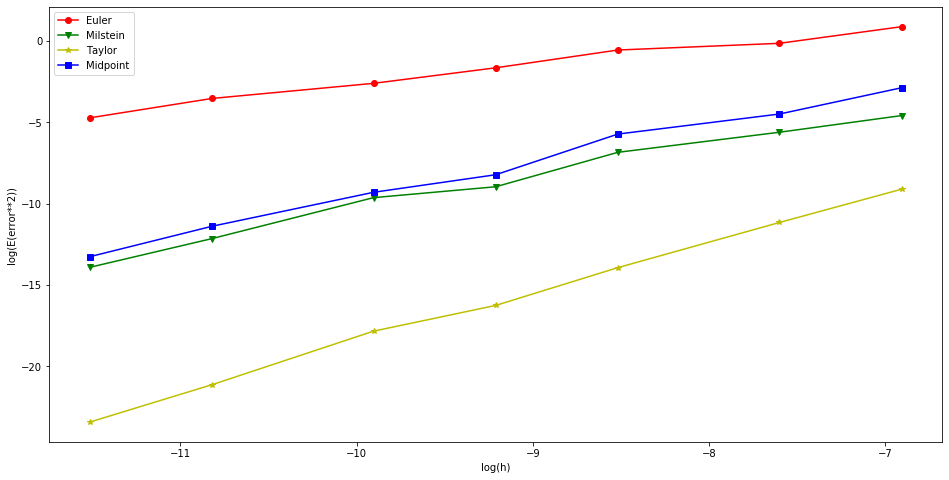
\includegraphics[width=2.95in]{images/6.2.png}}
	\vspace{.2cm}
	\caption{经典数值格式的收敛阶验证}
	\label{fig.6.1}
\end{figure}

测试过程选取了 $10^4$ 条样本轨道进行模拟,步长 $h\in[10^{-5},10^{-3}]$,相较于确定性的微分方程,其计算量大大增加. 根据定理3.1,可以得出 Euler-­Maruyama 格式具有0.5阶误差精度,而Milstein格式和中点公式均有1阶精度,Taylor格式具有最高的1.5阶精度. 中点公式属于隐格式,每次迭代需要求解方程,对于复杂的情况,中点公式的计算效率会受到影响. 

另一方面,估计误差的期望和方差使用 Monte Carlo 的方式,其本身就会存在 $\frac1{\sqrt N}$ 的误差,因此单纯减少步长 $h$ 的方式并不能完整说明数值格式的收敛阶. 对于 Euler-­Maruyama 格式,$N$ 至少与 $\frac1h$同阶,Milstein 格式或中点公式,$N = O(\frac1{h^{2}})$,而 Taylor 格式则是 $O(\frac1{h^{3}})$,因而上述数值实验中存在不可忽略的 Monte Carlo 导致的模拟误差. 

对 Ornstein–Uhlenbeck 方程:$\md X(t) = \mu X_t(t) \md t + \sigma \md B_t $,其真实解为
\[
X_{t}=X_{0} e^{\mu t}+\sigma \int_{0}^{t} e^{\mu(t-s)} \md B_{s}
\]
真实值与积分路径 $B_t$ 有关,而模拟时,数值积分本身就会引入误差,因此无法得到其真实解. 在文献\cite{OUequation}中,构造统计量将方程的参数与该方程的解联系起来. 



\section{稳定解的初值无关性与加速算法的验证}
本节验证4.3节提出的稳定解唯一时的初值无关性并实践加速算法. 考虑测试方程
\begin{equation}\label{example6.2}
\md x  = \left[ \tan(-\frac\pi2x) + \operatorname{sign}(x) \right] \md t + |1-|x||^\alpha \md B_t,\qquad x\in (-1,1).
\end{equation}
文献\cite{Fokker_Planck}指出,当$\alpha < \frac12$时,方程的扩散项不满足 H{\"o}lder 连续性,从而 SDE 的强解的存在唯一性无法保证,但仍然存在概率解. 数值实验考虑边界情况 $\alpha = \frac12$. 
使用Euler-Maruyama格式,对初值无关性的测试结果如下:
\begin{figure}[!htbp]
	\centering 
	\subfigure[$\mu_0 = \delta(\frac13)$]{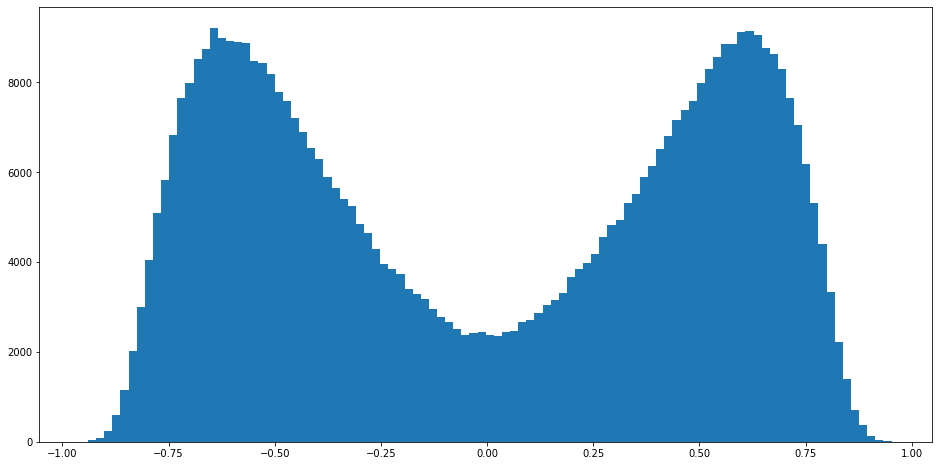
\includegraphics[width=1.95in]{images/6.2/1.png}}
	\subfigure[$\mu_0 = \frac12\delta(-\frac12)+\frac12\delta(\frac12)$]{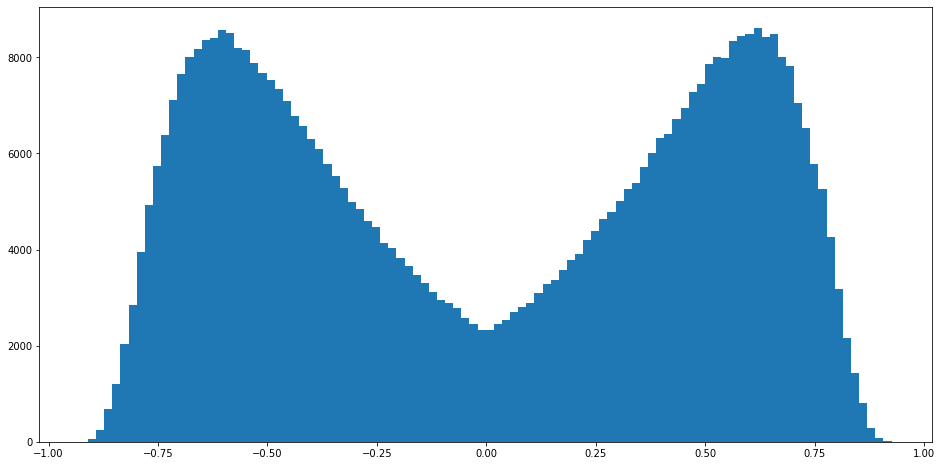
\includegraphics[width=1.95in]{images/6.2/2.png}}
	\subfigure[$\mu_0 = U(-0.999,0.999)$]{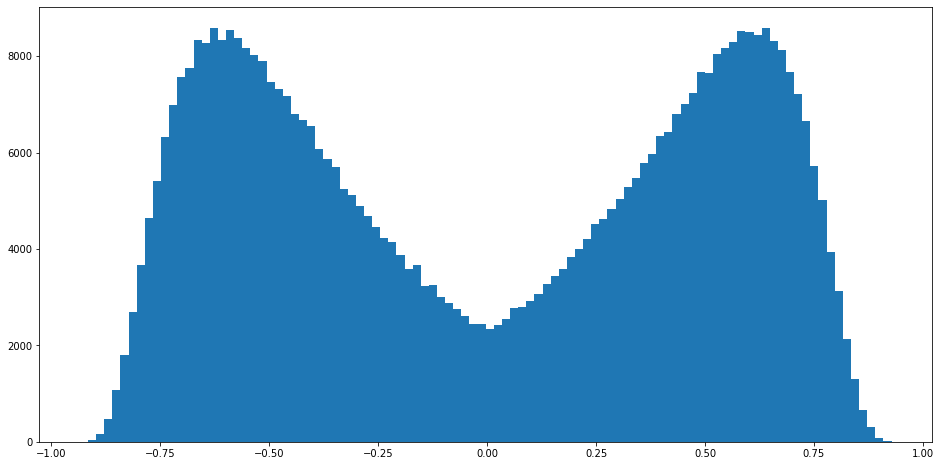
\includegraphics[width=1.95in]{images/6.2/3.png}}
	\vspace{.2cm}
	\caption{稳定解的初值无关性}
	\label{fig.6.2}
\end{figure}

图\ref{fig.6.2}表明,无论初始的分布选择有偏确定值、两点分布或者均匀分布,总是具有相同的稳定解. 注意到稳定解在0和$\pm1$附近的概率较小,而在$\pm0.7$附近拥有最大的概率密度. 结合方程的特点分析:
\begin{enumerate}
	\item[1] 当 $x\approx 0$ 时,方程漂移项较小,但扩散项较大,$x$ 很容易远离 $0$ 附近;
	\item[2] 当 $x\to 1^-$ 或 $x\to (-1)^+$ 时,扩散项很小,但漂移项较大且促使其向 0 移动;
	\item[3] 当 $x\approx 0.7$ 或 $x\approx -0.7$ 时,方程的漂移项和扩散项均不是非常大,$x$ 有更大概率停留,同时接受从0或$\pm1$附近移动过来的点. 
\end{enumerate}
稳定解反映的是随机系统中的粒子出现在各位置的概率值,粒子停留在系统中的时间越长,粒子越容易“遗忘”初始的信息. 

在求解自治随机微分方程时,如果系统存在稳定解,则分析较大的时间 $T$ 对应的概率解 $X_T$ 时,可以直接用稳定解代替. 一方面,随机微分方程计算其数值解时,对于较大的时间 $T$,计算代价会很大. 另一方面,由于稳定解的唯一性、指数收敛率以及加速算法,可以很快得到精度更高的解. 

对加速算法的实践见图\ref{fig.6.3},测试方程仍然取(\ref{example6.2}). 普通方法取步长 $h=10^{-2}$,320次模拟可以演化至 $T=3.20$. 加速算法取初始步长为 $h = \frac12$,每迭代 $\frac1{2h}$ 次后,步长 $h$ 减半,320次迭代可演化至 $T=4.125$,终止时步长 $h=\frac1{512}$. 
\begin{figure}[!htbp]
	\centering 
	\subfigure[$L^1$误差]{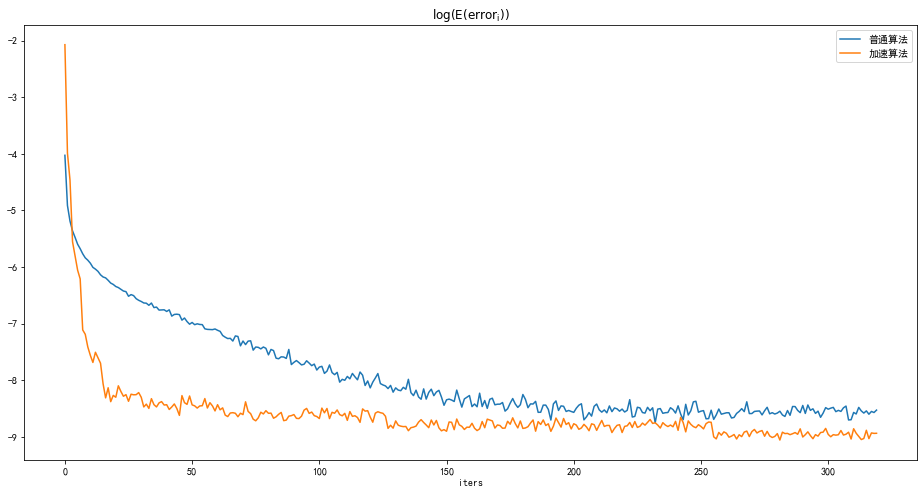
\includegraphics[width=5.95in]{images/6.2-result-1.png}}
	\subfigure[$L^2$误差]{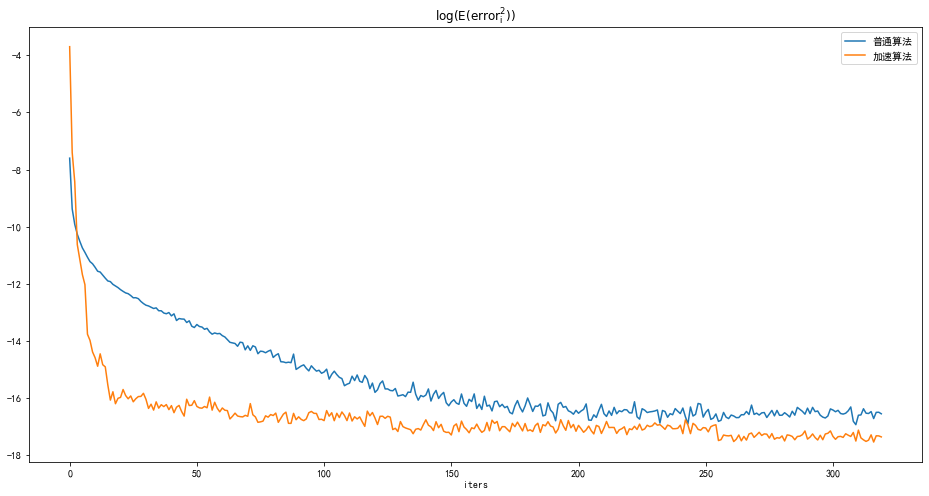
\includegraphics[width=5.95in]{images/6.2-result-2.png}}
	\vspace{.2cm}
	\caption{稳定解加速算法验证}
	\label{fig.6.3}
\end{figure}

由于无法求得稳定解的精确表达式,数值实验考虑相邻两次迭代之间的误差. 与确定性微分方程不同的是,$\md B_t = O(\sqrt{h})$,因此相邻两次迭代的样本轨道之间的误差会远大于 $h$. 假定概率解为 $X^*$,相邻两次的概率解为 $X_n$ 和 $X_{n+1}$,可以近似认为两概率解随机落在 $X^*$ 附近,即 $X_n,X_{n+1} \in Ball(X^*,r),r = \|X_{n+1} - X_n\|$. 


从误差的 $L^1$ 和 $L^2$ 范数的对数可以看出,算法刚开始时,加速算法以很快的速度远离初始分布,并很快到达稳定解附近. 随后随着步长 $h$ 的收缩越来越逼近稳定解. 而普通算法仅能以固定速度偏离初始分布,且时间足够长之后,因步长 $h$ 的限制,精度相较加速算法会显得不足. 






\section{例:二维随机 Kubo oscillator 方程}
本节验证带守恒量的自治随机微分方程的数值解法,对比经典方法和本文提出的算法,数值实验验证了本文提出的算法在保持守恒量方面的优势和数值精度上的变化,并指出本文提出的算法在求解稳定解方面的优势. 

考虑二维的例子:Kubo oscillator 方程:
\begin{equation}\label{eq_Kubo_ito}
\begin{aligned}
& \md x = \left(\frac12 \sigma^2 x(t) - by(t) \right)\md t -\sigma y(t)  \md B_t \\
& \md y =  \left(\frac12 \sigma^2 y(t)+ bx(t) \right)\md t + \sigma x(t)  \md B_t 
\end{aligned}
\end{equation}
其等价的 Stratonovich 型微分方程为
\begin{equation}\label{eq_Kubo_Str}
\begin{aligned}
& \md x = - by(t) \md t - \sigma y(t) \circ \md B_t \\
& \md y =   bx(t) \md t + \sigma x(t) \circ \md B_t 
\end{aligned}
\end{equation}
具有守恒量 $I(x,y) = x^2+y^2$. 有如下的单步数值格式:
\begin{enumerate}
	\item[$\bullet$] 直接差分方法
	\[
	\begin{aligned}
	x_{n+1} = x_n - by_nh - \sigma y_n \Delta_B \\
	y_{n+1} = y_n + bx_nh + \sigma x_n \Delta_B  
	\end{aligned}
	\]
	\item[$\bullet$] Euler-Maruyama 格式(0.5阶精度)
	\[
	\begin{aligned}
	x_{n+1} = x_n + (\frac12\sigma^2x_n-by_n)h - \sigma y_n \Delta_B \\
	y_{n+1} = y_n + (\frac12\sigma^2y_n+bx_n)h + \sigma x_n \Delta_B  
	\end{aligned}
	\]
	\item[$\bullet$] Milstein 格式(1阶精度)
	\[
	\begin{aligned}
	x_{n+1} = x_n + (\frac12\sigma^2x_n-by_n)h - \sigma y_n \Delta_B -\frac12\sigma^2x_n \Delta_B^2 \\
	y_{n+1} = y_n + (\frac12\sigma^2y_n+bx_n)h + \sigma x_n \Delta_B -\frac12\sigma^2y_n \Delta_B^2 
	\end{aligned}
	\]
	\item[$\bullet$] Taylor 格式(1.5阶精度)
	\[
	\begin{aligned}
	x_{n+1} = x_n &+ (\frac12\sigma^2x_n-by_n)h - \sigma y_n \Delta_B 
					 -\frac12\sigma^2x_n \Delta_B^2 
					+\frac16\sigma^3y_n(\Delta_B^3-3h\Delta_B)\\
				  &-(\frac12\sigma^3y_n+\sigma bx_n)h\Delta_B
				  +(\frac18\sigma^4x_n-\frac12\sigma^2by_n-\frac12b^2x_n)h^2\\
	y_{n+1} = y_n &+ (\frac12\sigma^2y_n+bx_n)h + \sigma x_n \Delta_B
					 -\frac12\sigma^2y_n \Delta_B^2 
					 -\frac16\sigma^3x_n(\Delta_B^3-3h\Delta_B)\\
				  &+(\frac12\sigma^3x_n-\sigma by_n)h\Delta_B
				  +(\frac18\sigma^4y_n+\frac12\sigma^2bx_n-\frac12b^2y_n)h^2
	\end{aligned}
	\]
\end{enumerate}
注意到直接差分方法并不等同于 Euler-Maruyama 格式,对于随机微分方程,二次变差项不能忽略. 
现考虑其守恒量,根据5.1节的格式(\ref{scheme_discrete_1})和(\ref{scheme_discrete_2}),推导保守恒量的数值格式. 取 
\[
\begin{aligned}
&S(x) =  \frac{f(x) \nabla I(x)^T - \nabla I(x) f(x)^T}{|\nabla I(x)|^2} \\
&T(x) =  \frac{g(x) \nabla I(x)^T - \nabla I(x) g(x)^T}{|\nabla I(x)|^2} 
\end{aligned}
\]
得
\[
S = \begin{pmatrix} 0&-b\\b&0\end{pmatrix}, \qquad
T = \begin{pmatrix} 0&-\sigma\\\sigma&0\end{pmatrix}
\]
因此二维 Kubo oscillator 方程的 SG 格式为:
\begin{equation}
	\md \begin{pmatrix} x(t) \\ y(t)	\end{pmatrix} = \frac12
	\begin{pmatrix} 0&-1 \\  1&0	\end{pmatrix} 
	\begin{pmatrix} I_x \\ I_y	\end{pmatrix} (b \md t + \sigma \md B_t).
\end{equation}
因 $S$ 为常系数矩阵,从而离散梯度格式(\ref{scheme_discrete_1})和(\ref{scheme_discrete_2}一致,为
\begin{equation}\label{scheme-SG}
\begin{aligned}
	&x_{n+1} = x_n - \frac b2(y_n+y_{n+1})h -\frac \sigma 2 (y_n+y_{n+1}) \Delta_B\\
	&y_{n+1} = y_n + \frac b2(x_n+x_{n+1})h +\frac \sigma 2 (x_n+x_{n+1}) \Delta_B
\end{aligned}
\end{equation}
上述格式为隐格式,但可以显式求解出来. 

考虑到该随机微分方程不存在精确解的表示式,使用Taylor方法的计算结果作为真值. 通过数值实验也验证了经典数值格式的误差精度,并说明格式(\ref{scheme-SG})同样具有一阶整体精度.

图\ref{fig.6.4}说明离散梯度格式具有1阶整体精度. 图\ref{fig.6.5}说明步长 $h$ 越小,守恒量偏离初始值的就越少,但除了离散梯度格式,其余算法均固定向某一个方向偏移,而离散梯度格式在所有的样本轨道上均能保持守恒量 $x^2+y^2$ 始终为1.图\ref{fig.6.6}取步长 $h=0.05$,数值结果说明随着时间增长,守恒量的偏移方向始终是一致的,因而时间越长,结果越不可取. 除了保持守恒量的离散梯度格式外,其余算法均呈现精度越高,守恒量误差也越少,这也是合理的. 

\begin{figure}[!htbp]
	\centering 
	\subfigure[$L^1$误差]{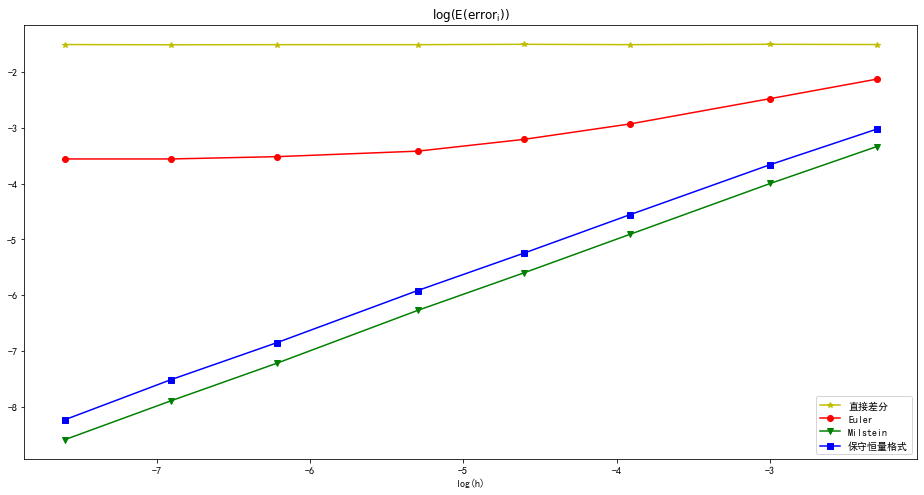
\includegraphics[width=2.95in]{images/6.3/1.png}}
	\subfigure[$L^2$误差]{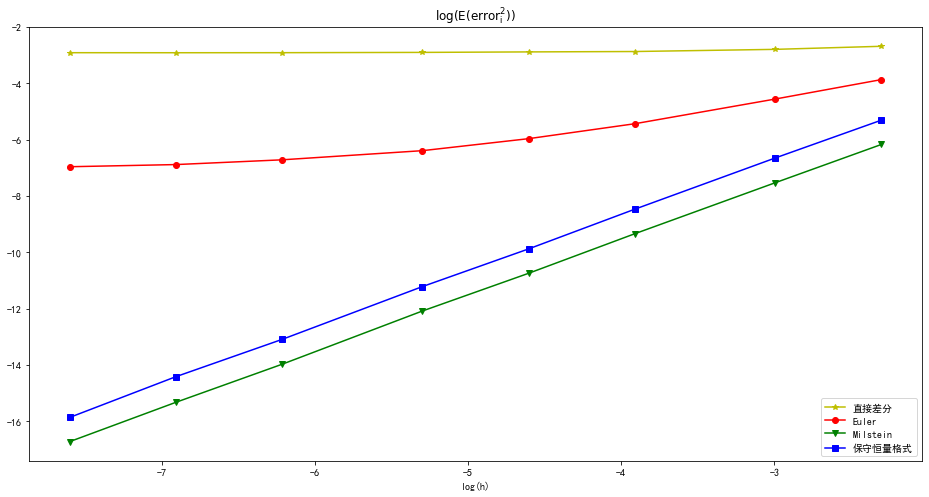
\includegraphics[width=2.95in]{images/6.3/2.png}}
	\vspace{.2cm}
	\caption{二维 Kubo oscillator 方程数值格式的误差}
	\label{fig.6.4}
\end{figure}

\begin{figure}[!htbp]
	\centering 
	\subfigure[守恒量的均值]{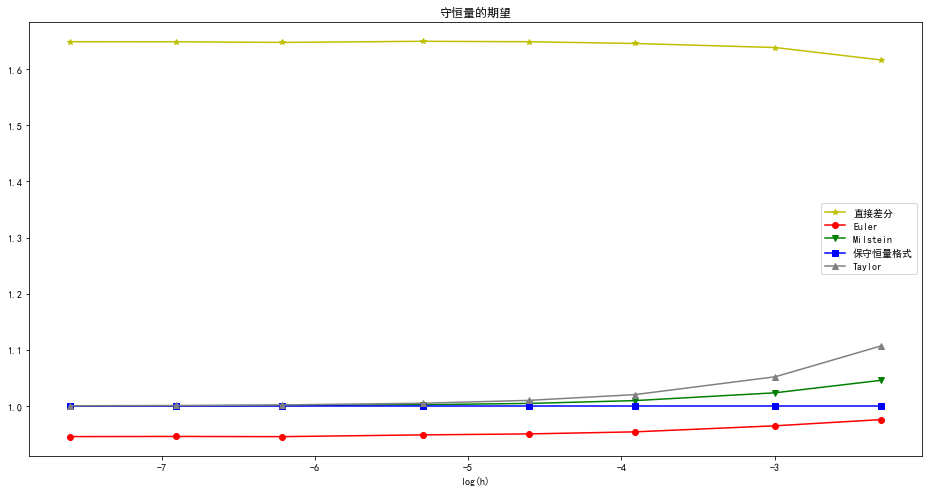
\includegraphics[width=2.95in]{images/6.3/3.png}}
	\subfigure[守恒量的方差]{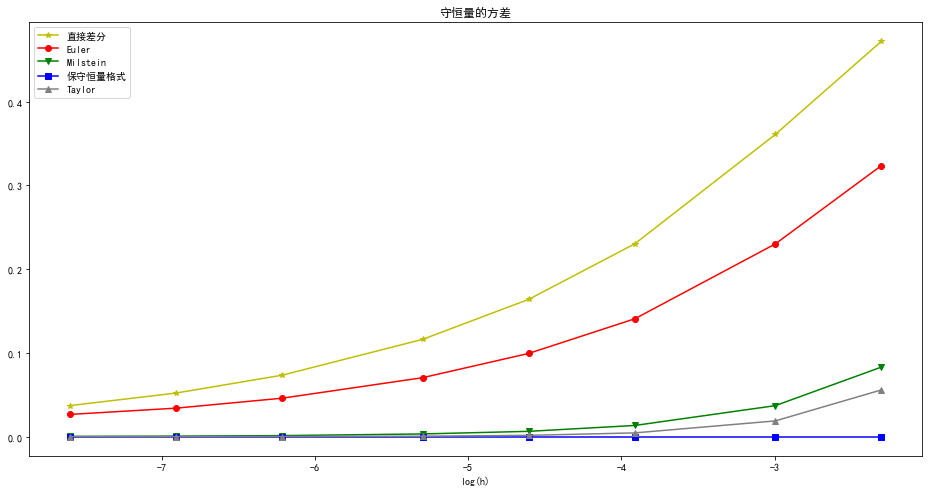
\includegraphics[width=2.95in]{images/6.3/4.png}}
	\vspace{.2cm}
	\caption{二维 Kubo oscillator 方程数值格式的守恒量}
	\label{fig.6.5}
\end{figure}




\begin{figure}[!htbp]
	\centering 
	\subfigure[守恒量的均值]{\includegraphics[width=2.95in]{images/6.3/5.png}}
	\subfigure[守恒量的方差]{\includegraphics[width=2.95in]{images/6.3/6.png}}
	\vspace{.2cm}
	\caption{二维 Kubo oscillator 方程守恒量随时间的变化}
	\label{fig.6.6}
\end{figure}



通过投射的思想,可以直接将单步法改造成对应的投射方法. 考虑到该守恒量对应的流形是单位圆周,因此可以直接选择投射到距离最近的点上. 考虑初值 $(x,y) = (1,0)$,步长 $h= 0.01$,对5000条样本轨道进行模拟,Euler格式、Milstein格式、EulerP格式结果如下:
\begin{figure}[!htbp]
	\centering 
	\subfigure[T=0.5]{\includegraphics[width=1.95in]{images/6.3/7(T=0.5).png}}
	%\subfigure[T=1.0]{\includegraphics[width=1.95in]{images/6.3/8(T=1).png}}
	\subfigure[T=5.0]{\includegraphics[width=1.95in]{images/6.3/9(T=5).png}}
	\subfigure[T=20.0]{\includegraphics[width=1.95in]{images/6.3/10(T=20).png}}
	\vspace{.2cm}
	\caption{Euler,Milstein,EulerP格式}
	\label{fig.6.7}
\end{figure}

模拟结果与图\ref{fig.6.6}一致,Euler 格式守恒量的方差要大得多,且守恒量均值略小于初始守恒量,而 Milstein 格式守恒量方差较小,均值略大于初始守恒量. 进一步分析 EulerP、MilsteinP 格式的收敛阶,由图\ref{fig.6.8}可以看出 EulerP、MilsteinP 的精度均比对应的单步方法 Euler格式、Milstein格式高. 
\begin{figure}[!htbp]
	\centering 
	\subfigure[守恒量的均值]{\includegraphics[width=2.95in]{images/6.3/11.png}}
	\subfigure[守恒量的方差]{\includegraphics[width=2.95in]{images/6.3/12.png}}
	\vspace{.2cm}
	\caption{二维 Kubo oscillator 方程守恒量随时间的变化}
	\label{fig.6.8}
\end{figure}


使用本文提出的加速算法演化(\ref{eq_Kubo_ito})的稳定解,由图\ref{fig.6.9}可以看出,该随机系统达到稳定状态时,粒子在 $\pm 1$ 附近出现的概率更大,并且 $X,Y$ 的稳定解几乎是一致的. 但值得注意的是,这边的数值格式必须要保持守恒量不变,否则不满足 $(x,y) \in [-1,1]\times [-1,1]$ 的条件,因而绝对不可能得到图\ref{fig.6.9}的稳定结果. 

\

\begin{figure}[!htbp]
	\centering 
	\subfigure{\includegraphics[width=2.95in]{images/Kubo/kubo-x.png}}
	\subfigure{\includegraphics[width=2.95in]{images/Kubo/kubo-y.png}}
	\vspace{.2cm}
	\caption{二维 Kubo oscillator 方程的稳定解}
	\label{fig.6.9}
\end{figure}




对问题(\ref{eq_Kubo_Str})做坐标旋转,得
\[
\md 
\begin{pmatrix} x\\y\end{pmatrix}
\begin{pmatrix} \cos \theta & \sin \theta \\ -\sin \theta & \cos \theta \end{pmatrix}
= 
\begin{pmatrix} 0&-1 \\  1&0	\end{pmatrix} 
\begin{pmatrix} x \\ y	\end{pmatrix} 
\begin{pmatrix} \cos \theta & \sin \theta \\ -\sin \theta & \cos \theta \end{pmatrix}
(b \md t + \sigma \md B_t).
\]
与坐标旋转之前具有一致的微分形式,故 $(x,y)$ 具有旋转对称性. 因此稳定解 $(x,y)$ 是守恒量对应的流形上的均匀分布,则概率密度函数为:
\[
P (x=a) = \frac{1}{\pi\sqrt{1-a^2}},\qquad P(y=b) = \frac{1}{\pi\sqrt{1-b^2}}.
\]
其在区间 $[t_n,t_{n+1}]$ 上的概率值为 $\frac1\pi\left(\operatorname{arcsin}(t_{n+1}) - \operatorname{arcsin}{(t_{n})}\right)$. 其概率分布柱状图如下. 
\begin{figure}[!htbp]
	\centering 
	\subfigure{\includegraphics[width=2.95in]{images/Kubo/thoery_hist.png}}
	\vspace{.2cm}
	\label{fig.6.10}
\end{figure}
与模拟的结果也是一致的. 因此在求解该自治随机微分方程时,稳定解为圆周上的均匀分布,且不论初值情况如何,对 $T>1$ 的情况,可以直接用稳定解代替数值格式得到的解. 
即对演化时间足够长的情况,概率解为
\begin{equation}
\mu_{_T}(x,y) \approx
\left\{
\begin{aligned}
&\frac1{2\pi \sqrt{x_0^2+y_0^2}}, \qquad  & \rm{if}\quad x^2+y^2=x_0^2+y_0^2,\\
& 0,\qquad  & \rm{if}\quad x^2+y^2\neq x_0^2+y_0^2 .
\end{aligned}
\right.
\end{equation}

在离散操作过程中,不考虑守恒量时无法注意到该方程存在稳定解. 但使用保持守恒量的数值格式,则很容易得到该方程的稳定解. 这说明对于演化过程较长的情况,引入守恒量对概率解精度的提升是非常巨大的. 由稳定解的唯一性和指数收敛的特性,使用保守恒量的数值格式计算得到的稳定解的误差是有界的. 
并且可以做出如下猜想:当自治随机微分方程存在守恒量,且守恒量对应的流形的测度有限时,只要存在概率解,就必定存在唯一的稳定解. 


\section{例:三维随机 Lotka Volterra 方程}
本节通过高维的例子验证间接离散梯度算法的有效性. 考虑三维随机 Lotka Volterra 方程,
\begin{equation}\label{eq6.7}
\md 
\begin{pmatrix} x \\y \\z \end{pmatrix}
=
\begin{pmatrix}x(z-y) \\y(x-z) \\z(y-x)\end{pmatrix} \md t
+
\begin{pmatrix} x(z-y) \\y(x-z) \\z(y-x)\end{pmatrix} \circ \md B_t
\end{equation}
具有守恒量 $I(x,y,z) = x+y+z$. 
此处为了格式的简洁,不考虑 \ito 意义下的微分方程. 
由于该方程同样不存在精确解的表达式,且 Taylor 格式存在不可积分项,无法写出,因此本节的参照格式为 Milstein 格式. 计算 $\frac12 \frac {\partial g(X)}{\partial X} g(X)$,得其格式:
\[
\begin{aligned}
&x_{n+1}=x_{n}+x_{n}\left(z_{n}-y_{n}\right)(h+\Delta _B)
	+\frac{1}{2}\left(x_{n}\left(y_{n}^{2}+z_{n}^{2}-x_{n}\left(y_{n}+z_{n}\right)\right)\right) \Delta_B^2\\
&y_{n+1}=y_{n}+y_{n}\left(x_{n}-z_{n}\right)(h+\Delta _B)
	+\frac{1}{2}\left(y_{n}\left(z_{n}^{2}+x_{n}^{2}-y_{n}\left(x_{n}+z_{n}\right)\right)\right) \Delta_B^2\\
&z_{n+1}=z_{n}+z_{n}\left(y_{n}-x_{n}\right)(h+\Delta _B)
	+\frac{1}{2}\left(z_{n}\left(x_{n}^{2}+y_{n}^{2}-z_{n}\left(x_{n}+y_{n}\right)\right)\right)\Delta_B^2
\end{aligned}
\]
再分析其 SG形式为:
\begin{equation}\label{eq6.9}
\md\left(\begin{array}{l}
	x \\
	y \\
	z
\end{array}\right)=\left(\begin{array}{ccc}
	0 & -\frac{2 x y-x z-y z}{3} & -\frac{x y+y z-2 x z}{3} \\
	\frac{2 x y-x z-y z}{3} & 0 & -\frac{2 y z-x y-x z}{3} \\
	\frac{x y+y z-2 x z}{3} & \frac{2 y z-x y-x z}{3} & 0
\end{array}\right)\left(\begin{array}{l}
	1 \\
	1 \\
	1
\end{array}\right)(\md t + \circ  \md B_t)
\end{equation}
将其拆解为如下三个子系统
\begin{align*}
\left\{
\begin{array}{l}
\md\left(\begin{array}{l}
x \\
y
\end{array}\right)=\left(\begin{array}{cc}
0 & -\frac{2 x y-x z-y z}{3} \\
\frac{2 x y-x z-y z}{3} & 0
\end{array}\right)\left(\begin{array}{l}
1 \\
1
\end{array}\right)(\md t + \circ \md B_t) \\
\md z=0
\end{array}       
\right.        \tag{\ref{eq6.9}{.a}}\\
\left\{\begin{array}{l}
\md\left(\begin{array}{c}
x \\
z
\end{array}\right)=\left(\begin{array}{cc}
0 & -\frac{x y+y z-2 x z}{3} \\
\frac{x y+y z-2 x z}{3} & 0
\end{array}\right)\left(\begin{array}{l}
1 \\
1
\end{array}\right)(\md t + \circ \md B_t) \\
\md y=0
\end{array}
\right.        \tag{\ref{eq6.9}{.b}}\\
\left\{
\begin{array}{l}
\md\left(\begin{array}{l}
y \\
z
\end{array}\right)=\left(\begin{array}{cc}
0 & -\frac{2 y z-x y-x z}{3} \\
\frac{2 y z-x y-x z}{3} & 0
\end{array}\right)\left(\begin{array}{l}
1 \\
1
\end{array}\right)(\md t + \circ \md B_t) \\
\md x=0
\end{array}     
\right.        \tag{\ref{eq6.9}{.c}}
\end{align*}
使用隐格式 (\ref{scheme_discrete_1})或(\ref{scheme_discrete_2})处理上述三个子系统,均不能得到显式表达式. 使用非线性求解器求解隐格式,效率则会下降很多,数值实验表明,该格式尽管可以保证误差精度,但并不能得到一个稳定解. 这是因为方程(\ref{eq6.7})还存在另一个守恒量 $I_2(x,y,z) = xyz$,而SG形式不能处理带多个守恒量的问题. 投射方式采用到守恒量流形的 $L^2$ 距离最小的方式选取. 使用拉格朗日乘子法,得拉格朗日函数:
\[
L(x,y,z,\lambda_1,\lambda_2) = \frac12\left[
(x-x^*)^2+(y-y^*)^2+(z-z^*)^2
\right]
+\lambda_1(x+y+z-I) +  \lambda_2(xyz-I_2).
\]
数值实验很好的验证了该数值格式的精度和对守恒量保持的特性. 
\begin{figure}[!htbp]
	\centering 
	\subfigure{\includegraphics[width=5.95in]{images/Lotka/Figure_2.png}}
	\vspace{.2cm}
	\caption{三维随机 Lotka Volterra 方程的解}
	\label{fig.6.11}
\end{figure}
数值模拟得到 $I=4,I_2=2$ 时方程的稳定解,比对6.3节二维实验的结果,可以近似认为稳定解是守恒量对应的流形上的均匀分布. 
\begin{figure}[!htbp]
	\centering 
	\subfigure[X的稳定解]{\includegraphics[width=1.95in]{images/Lotka/x.png}}
	\subfigure[Y的稳定解]{\includegraphics[width=1.95in]{images/Lotka/y.png}}
	\subfigure[Z的稳定解]{\includegraphics[width=1.95in]{images/Lotka/z.png}}
	\vspace{.2cm}
	\caption{三维随机 Lotka Volterra 方程的稳定解}
	\label{fig.6.12}
\end{figure}

















 % 数值实验
  % !TeX encoding = UTF-8
\chapter{总结与展望}\label{chap7}


本文探究自治随机偏微分方程的数值解,由于其同时具有偏微分方程和随机过程的属性,分别从单一样本轨道的数值解和整体的概率解两个维度进行分析. 
对于时间 $T$ 较小的情况,本文综述经典的数值算法:Euler-Maruyama 格式、Milstein 格式、Taylor格式等. 并对带守恒量的问题介绍了维持守恒量的数值格式和投射算法. 
对于时间 $T$ 较大的情况,本文介绍其具有稳定概率分布的条件. 并分析当自治随机偏微分方程存在守恒量时,稳定解必然不唯一. 
本文的创新点在于探究带守恒量的问题时,对于单一样本轨道的数值解提出新的投射方法,对于整体的概率解,提出了稳定解不唯一并给出了能收敛到初值对应的稳定解的加速算法. 

通过实验,本文发现当状态“连通”且“连通”的状态的总测度有限时,SDE 总是存在稳定解. 带守恒量的问题稳定解不唯一是因为守恒量破坏了各状态之间的“连通性”,但本文没有分析探究这种“连通性”. 
另外本文的随机微分方程仅考虑了布朗运动的随机项 $B_t$,而更一般的分数阶布朗运动的随机项则未进行理论分析和相关实验. 可以推测的是,一般的分数阶布朗运动由于“时间记忆”的特点,即使存在稳定解,收敛速度也会更慢. 
这些有趣的角度非常值得进行进一步进行探究. 




% 发散:初值的扰动与混沌 
% 尝试 Fokker-Planck 方程的求解
 % 总结与展望

%\fi
%==============================================================

%\iffalse
  \backmatter %结束章节自动编号

%参考文献(习惯使用bibtex的可以修改)
  \addcontentsline{toc}{chapter}{参考文献} % 解决目录中没有相应的参考文献的条目问题
  \chaptermark{参考文献}
  %
\begin{thebibliography}{200}
    \bibitem{article1} Ernest P . The philosophy of mathematics education by Paul Ernest[J]. Social Epistemology.

    \bibitem{article2} Bishop A J. Mathematical enculturation: a cultural perspective on mathematics education[J]. Journal for Research in Mathematics Education, 1988, 20(4):195.


\end{thebibliography}

 
  \nocite{*}
  \bibliographystyle{plain} % siam , abbrv , plain zjuthesis.cls - 参考文献样式
  %\bibliography{chapters/bib}
  
  \bibliography{chapters/Ref}
  

%附录
   % !TeX encoding = UTF-8
\chapter{附录}
\section*{部分实验代码}
\subsection*{3.2节 Euler格式的python代码}

\scriptsize{
\begin{lstlisting}[style=styleP]
'''
d X = bX dt + sigma X dB
方程参数: X0,b,sigma
时间参数:T
格式参数:h
'''
import numpy as np
import matplotlib.pyplot as plt

class Euler():
	def __init__(self,X0,b,sigma,h,T):
		self.X0 = X0
		self.b,self.sigma = b,sigma
		self.h,self.T = h,T
		self.set_para()

	def set_para(self):
		self.N = int(self.T / self.h)
		self.sqrt_h = np.sqrt(self.h)
		self.t = [self.h * i for i in range(self.N+1)]
	
	def sample(self , myplot = 0):
		self.Brown = np.random.normal(0 , 1, self.N) * self.sqrt_h
		X = [self.X0 for i in range(self.N+1)]
		
		for i in range(self.N):
			X[i+1] = X[i] + self.b * X[i] * self.h + self.sigma * X[i] * self.Brown[i]
		
		if myplot:
			plt.figure(figsize=(20,10))
			plt.plot(self.t,X)
		
		real = self.X0 * np.exp((self.b-self.sigma**2/2)*self.T+self.sigma*np.sum(self.Brown))
		return (X[-1] , real)
	
	def test(self):
		EX = self.X0 * np.exp(self.b * self.T)
		DX = (self.X0**2 * np.exp(2*self.b*self.T) * (np.exp(self.sigma**2*self.T)-1))

		result,error = [],[]
		for i in range(10000):
			calc,real = self.sample()
			result.append(calc)
			error.append(real-calc)
		
		m_mean,m_std = np.mean(result),np.std(result) 
		print(EX , DX , '\n' , m_mean , m_std ** 2)
		print(np.mean(error) , np.std(error)**2)
		
		result = [ x for x in result if x > m_mean-5*m_std and x < m_mean + 5*m_std]
		plt.hist(result,bins = 100)

method = Euler(X0 = 2 , b = -2, sigma = 2 , h = 1e-4 , T = 5)
method.sample(myplot = 1)
method.test()
\end{lstlisting}
}



\subsection*{4.2节代码}
\scriptsize{
\begin{lstlisting}[style=styleP]
'''
方程:dX = bx dt + sqrt(2)*(1-x**2) dB
固定参数:b
可变参数:T
精度参数:h,格式
'''
import numpy as np
import matplotlib.pyplot as plt

class Stable():
	def __init__(self,b,h,T):
		self.b = b
		self.h = h
		self.T = T
		self.set_para()

	def set_para(self):
		self.N = int(self.T / self.h)
		self.sqrt_h = np.sqrt(self.h)
		self.sqrt_2 = np.sqrt(2)
		self.t = [self.h * i for i in range(self.N+1)]

	def sample(self,myplot = 0):
		self.Brown = np.random.normal(0 , 1, self.N) * self.sqrt_h
		X = [0 for i in range(self.N+1)]
		
		tmp = np.random.normal(0,0.2)
		while np.abs(tmp) >= 1:
			tmp = np.random.normal(0,0.2)
		X[0] = tmp        
			
		
		for i in range(self.N):
		# Milstein 格式
		X[i+1] = X[i] + self.b * X[i] * self.h + self.sqrt_2 * (1-X[i]**2) * self.Brown[i]
		X[i+1]+= (self.Brown[i]**2 - self.h) * 2 * X[i] * (X[i]**2-1)
		
		if X[i+1] > 1: X[i+1] = (X[i]+1) / 2
		if X[i+1] <-1: X[i+1] = (X[i]-1) / 2
		
		if myplot:
			plt.figure(figsize=(20,10))
			plt.plot(self.t,X)
		
		return X[-1]

	def measure(self):
		result = []
		for idx in range(500000):
			if idx % 20000 == 0: print(idx//5000+4)
			result.append(self.sample())
			
		plt.figure(figsize=(18,9))
		plt.xlim(-1,1)
		plt.hist(result , bins = 250)
		plt.show()

m = Stable(b = -2 , h = T/1000 , T = 1.0)
#m.sample(myplot=1)
m.measure()
\end{lstlisting}
}






\newpage

\subsection*{TaylorP格式下Kubo-oscillator 方程稳定解算法}
\scriptsize{
\begin{lstlisting}[style=styleP]
import os 
import numpy as np
import matplotlib.pyplot as plt
import pandas as pd

class Kubo():
	def __init__(self):
		self.b, self.sigma = 2,2
		self.h = 1e-2
		self.T = 80
	
	# 数据分布演化 num 次 
	def scheme(self,oldx,oldy,num):
		length = len(oldx)
		b,sigma,h = self.b , self.sigma, self.h
	
		newx,newy = [],[]
		for k in range(length):
			# 第 k 个点的模拟
			tx = [oldx[k] for _ in range(num+1)]
			ty = [oldy[k] for _ in range(num+1)]
			Brown = np.random.normal(0 , 1, self.N) * np.sqrt(self.h)
			for i in range(num):
				# Taylor格式
				tx[i+1] = tx[i] - b*ty[i]*h - sigma*ty[i]*Brown[i] - sigma**2*tx[i]/2*Brown[i]**2
				tx[i+1] +=(Brown[i]**3-3*h*Brown[i])/6 * sigma**3*ty[i]
				tx[i+1] +=(sigma**4/4*tx[i]-sigma**2*b*ty[i]-b**2*tx[i])/2*h*h
				tx[i+1] -= Brown[i]*h*(sigma**3/2*ty[i]+b*sigma*tx[i])
				ty[i+1] = ty[i] + b*tx[i]*h + sigma*tx[i]*Brown[i] - sigma**2*ty[i]/2*Brown[i]**2
				ty[i+1] -=(Brown[i]**3-3*h*Brown[i])/6 * sigma**3*tx[i]
				ty[i+1] +=(sigma**4/4*ty[i]+sigma**2*b*tx[i]-b**2*ty[i])/2*h*h
				ty[i+1] += Brown[i]*h*(sigma**3/2*tx[i]-b*sigma*ty[i])
				# 投射操作
				tmp = np.sqrt(tx[i+1]**2 + ty[i+1]**2)
				tx[i+1],ty[i+1] = tx[i+1]/tmp,ty[i+1]/tmp

			newx.append(tx[-1])
			newy.append(ty[-1])
		
		return newx,newy
	
	def test(self):
		num = int(0.2 / self.h)
		
		for n in range(1,int(self.T/0.2)+1):
			time = str(n*2//10).zfill(2)+'.'+str(n*2%10)
			print(time)
			if 'T='+time+'.csv' in os.listdir('D:\data\Kubo\point'):
				data = pd.read_csv('D:\data\Kubo\point\T='+time+'.csv')
				x = list(data['x'])
				y = list(data['y'])
				continue
		
			x,y = self.scheme(x,y,num)
			out = pd.DataFrame({'x':x , 'y':y})
			out.to_csv('D:\data\Kubo\point\T='+time+'.csv')
			
			plt.hist(x,bins = 100)
			plt.savefig('D:\data\Kubo\histX\T='+time+'.png')
			plt.show()
			
			plt.hist(y,bins = 100)
			plt.savefig('D:\data\Kubo\histY\T='+time+'.png')
			plt.show()
			
			plt.figure(figsize=(8,8))
			plt.scatter(x[:100],y[:100])
			plt.show()

k = Kubo()
k.test()
\end{lstlisting}
}







\section*{\ito 积分、Stratonovich积分下的二次变差项}
随机积分中,积分表达式 $\displaystyle \int B_t \md B_t$ 会多次出现. 同时注意到,本文的理论与数值格式中,$\frac12 \Delta B_t^2$ 这类二次变差项也会反复出现. 且在\ito 积分、Stratonovich积分下正负号正好相反. 此处简要计算说明. 
\[
\begin{aligned} 
S_{n}&=\sum_{i=0}^{n-1} B\left(t_{i}^{n}\right)\left[B\left(t_{i+1}^{n}\right)-B\left(t_{i}^{n}\right)\right] \\
&=
\sum_{i=0}^{n-1} \frac{B\left(t_{i+1}^{n}\right)+B\left(t_{i}^{n}\right)}{2}\left[B\left(t_{i+1}^{n}\right)-B\left(t_{i}^{n}\right)\right] 
-\sum_{i=0}^{n-1} \frac{B\left(t_{i+1}^{n}\right)-B\left(t_{i}^{n}\right)}{2}\left[B\left(t_{i+1}^{n}\right)-B\left(t_{i}^{n}\right)\right]\\
&=\frac12 B(T)^2 - \frac12 \sum_{i=0}^{n-1}\left[B\left(t_{i+1}^{n}\right)-B\left(t_{i}^{n}\right)\right]^{2} 
\longrightarrow \frac12 B(T)^2 - \frac12 T.\\
S^{\prime}_n&=\sum_{i=0}^{n-1} B\left(t_{i+1}^{n}\right)\left[B\left(t_{i+1}^{n}\right)-B\left(t_{i}^{n}\right)\right]
\longrightarrow \frac12 B(T)^2 + \frac12 T.\\
S_n''&=\sum_{i=0}^{n-1} \frac{B\left(t_{i+1}^{n}\right)+B\left(t_{i}^{n}\right)}{2}\left[B\left(t_{i+1}^{n}\right)-B\left(t_{i}^{n}\right)\right] = \frac12 B(T)^2
\end{aligned}
\]
第一种情况对应 \ito 积分意义,第二中情况对应 Stratonovich 积分意义. 


\iffalse


\begin{shaded}
	积分表计算:文献\cite{integer}
\end{shaded}


\section*{积分表}
下面的积分表用于数值积分的推导
\begin{table}[!htbp]
\caption{随机积分表}
\centering
\begin{tabular}{c|c||c|c}
	\ito 积分表达式 & 值 & Stratonovich 积分 & 值 \\
	\hline
	\rule{0pt}{15pt}$\int_t^{t+h} \md B_s$  & $\Delta B$  & 
		$\int_t^{t+h} \circ \md B_s$  & $\Delta B$   \\
	\rule{0pt}{15pt}$\int_t^{t+h} \int_t^s \md B_\theta \md s $ & $\Delta Z$ & 
		$\int_t^{t+h} \int_t^s \circ \md B_\theta \md s $ & $\Delta Z$ \\
	\rule{0pt}{15pt} $\int_t^{t+h}\int_t^s \md \theta \md B_s $ & $\Delta B \cdot h - \Delta Z$ &
		$\int_t^{t+h}\int_t^s \md \theta \circ\md B_s $ & $\Delta B \cdot h - \Delta Z$ \\
	\rule{0pt}{15pt} $\int_t^{t+h} \int_t^s \md B^1_\theta \md B^2_s$
\end{tabular}
\end{table}

\fi








% 出版物
   % 111

% 作者简历
  \chapter*{\centerline{作者简历}}
\chaptermark{作者简历}
\addcontentsline{toc}{chapter}{作者简历}


张少杰,男,1996年,汉族,浙江杭州人。2014年考入浙江大学数学科学学院(数学与应用数学专业),2018年本科毕业,获得理学学士学位。2018年进入浙江大学数学科学学院计算数学专业研究生学习至今。

\begin{enumerate}
    %\item 工作经历
    %\begin{itemize}
    %    \item 2019年,在华为技术有限公司2012实验室担任通用软件开发工程师
    %\end{itemize}

	
    \item 参与的项目
    \begin{itemize}
        \item 2020年,参与浙大阿里城市级跨摄像头车辆重识别技术项目
    \end{itemize}

	\item 奖励荣誉
	\begin{itemize}
		\item 2019年03月,阿里巴巴全球数学竞赛优胜奖
		\item 2019年11月,研究生国家奖学金
		\item 2019年11月,浙江大学优秀研究生
	\end{itemize}

    %\item 攻读学位期间发表的论文
\end{enumerate}


%\fi

\end{document}
